% This is a LaTeX thesis template for Monash University.
% to be used with Rmarkdown
% This template was produced by Rob Hyndman
% Version: 6 September 2016

\documentclass{template/monashthesis}

%%%%%%%%%%%%%%%%%%%%%%%%%%%%%%%%%%%%%%%%%%%%%%%%%%%%%%%%%%%%%%%
% Add any LaTeX packages and other preamble here if required
%%%%%%%%%%%%%%%%%%%%%%%%%%%%%%%%%%%%%%%%%%%%%%%%%%%%%%%%%%%%%%%

\usepackage{thumbpdf,lmodern}
\usepackage{amsmath}
\usepackage{bm}
\usepackage{booktabs}
%%%% NS
%\usepackage{mathtools,amssymb,booktabs,amsthm,todonotes,colortbl,amsthm,multirow,array} %% blind c+p from sayani
\usepackage{ragged2e} %% declaration table RaggedRight
\usepackage{graphicx}
%\usepackage{pdflscape} %% Allow landscape layout, not used
%\usepackage{lmodern} %% Already loaded, allows GB Pound sign
%\usepackage{animate} %% Needed for animations
\PassOptionsToPackage{hyphens}{url}\usepackage{hyperref} %% Trying to wrap and format urls correctly

\author{Nicholas S Spyrison}
\title{Interactive and dynamic visualization of high-dimensional data via animated linear projections, their efficacy, and their application to local explanations of non-linear models}
\degrees{B.Sc. Statistics, Iowa State University}
\def\degreetitle{Doctor of Philosophy}
% Add subject and keywords below
\hypersetup{
     %pdfsubject={The Subject},
     %pdfkeywords={Some Keywords},
     pdfauthor={Nicholas S Spyrison},
     pdftitle={Interactive and dynamic visualization of high-dimensional data via animated linear projections, their efficacy, and their application to local explanations of non-linear models},
     pdfproducer={Bookdown with LaTeX}
}

\bibliography{thesisrefs}

\begin{document}

\pagenumbering{roman}

\titlepage

{\setstretch{1.2}\sf\tighttoc\doublespacing}

\hypertarget{ch-copyright}{%
\chapter*{Copyright notice}\label{ch-copyright}}
\addcontentsline{toc}{chapter}{Copyright notice}

\textcopyright { }Nicholas Spyrison (\number\the\year).

I certify that I have made all reasonable efforts to secure copyright permissions for third-party content included in this thesis and have not knowingly added copyright content to my work without the owner's permission.

\newpage

\hypertarget{abstract}{%
\chapter*{Abstract}\label{abstract}}
\addcontentsline{toc}{chapter}{Abstract}

Visualizing data space is crucial to exploratory data analysis, checking model assumptions, and validating model performance. Yet visualization quickly becomes difficult as the dimensionality of the data or features increases. Traditionally, static, low-dimensional linear embeddings are used to mitigate this complexity. Such embedded space is a lossy approximation of the full space. However, viewing many embeddings with interactive supporting views, maximizes the information conveyed. Data visualization \emph{tours} are a class of dynamic linear projections that animate many linear projections over small changes to the projection basis.

Tours are categorized by the path of their bases. \emph{Manual tours} allow for User-Controlled Steering (UCS) of bases path, where the contributions of individual variables can be controlled. I create a free, open-source \textbf{R} package, \textbf{spinifex} that facilitates the creation of such tours. These manipulations of the variables can be precomputed or made in real-time. The animations are interoperable with the existing package \textbf{tourr} and can be rendered with recent graphics interfaces \textbf{plotly} and \textbf{gganimate}. The former offers interactive use with HTML widgets while the latter can render to static formats such as .gif or .mp4 files. An interactive application is included to illustrate the use of the manual tour.

Theoretically, UCS of the manual tour should enable an analyst to better explore the variable attribution to the structure identified in an embedding. I find strong evidence to support that radial tour leads to a significant and large increase in accuracay as compared with Principal Component Analysis (PCA) and an alternative tour variant, the grand tour. I conduct a within-participant, crowd-sourced user study comparing these visualization methods. Each of the \(n=108\) participants performs two trials with each visual for 648 total trials. The task is a supervised classification problem asking participants which variables attribute to the separation of 2 clusters.

Modern modeling techniques are sometimes referred to as black-box models due to the uninterpretable nature of model terms which are often many and non-linear. Recent research in Explainable Artificial Intelligence (XAI) tries to bring interpretability to these models through the use of \emph{local explanations}. Local explanations are a class of techniques that approximate the linear-variable importance at one point in the data. I build an \textbf{cheem}, an \textbf{R} package to streamline model and local explanation preprocessing and two novel visuals. First the global view pits the data- and explanation-spaces side-by-side with a residual plot. Interactive features such as linked bushing and tooltips aid in the identification of observations to compare. The local explanation from the selected observation becomes a basis used in the creation of the radial tour. This allows us to evaluate the explanation and see explore how sensitive the explanation is to changes in the variable contribution.

\clearpage\pagenumbering{arabic}\setcounter{page}{0}

\hypertarget{declaration}{%
\chapter*{Declaration}\label{declaration}}
\addcontentsline{toc}{chapter}{Declaration}

I hereby declare that this thesis contains no material which has been accepted for the award of any other degree or diploma at any university or equivalent institution and that, to the best of my knowledge and belief, this thesis contains no material previously published or written by another person, except where due reference is made in the text of the thesis.

Three publications are included in this thesis, one of which has been accepted for publication in \emph{The R Journal} \autocite{spyrison_spinifex_2020}. The user study described in Chapter \ref{ch:efficacy_radial_tour} will shortly be submitted to the \emph{Journal of Data Science, Statistics, and Visualisation}. The research covered in Chapter \ref{ch:cheem} will shortly be submitted to \emph{IEEE Transactions on Knowledge and Data Engineering}.

All of the papers in the thesis were conceptualized, developed, and written by myself, the student, while working in the Department of Human-Centred Computing under the supervision of professor Kimbal Marriott and professor Dianne Cook. When co-authors are listed, it indicates that the work was produced through active collaboration between researchers and that their contributions to team-based research have been recognized. The following table details the work, including my and my fellow co-authors' contributions.

\begin{table}
\centering\footnotesize\tabcolsep=0.12cm
\begin{tabular}{|p{1cm}|p{2cm}|p{1.5cm}|p{3.5cm}|p{3.5cm}|p{1.5cm}|}
\hline
\RaggedRight\textbf{Thesis Chapter}  &
\RaggedRight\textbf{Publication Title}  &
\RaggedRight\textbf{Status (published, in press, accepted or returned for revision)}  & \RaggedRight\textbf{Nature and} {\%} \RaggedRight\textbf{of student contribution} & \RaggedRight\textbf{Co-author name(s) Nature and} {\%} \RaggedRight\textbf{of Co-author’s contribution} &
\RaggedRight\textbf{Co-author(s), Monash student Y/N} \\ \hline
3 & spinifex: An R Package for Creating a Manual Tour of Low-dimensional Projections of Multivariate Data & Published & 75\%. Concept, development, writing first draft and software development & (1) Dianne Cook, concept, methodology, writing 25\% & N \\ \hline
4 & The benefit of user-controlled radial tour for understanding variable contributions to structure in linear projections & To be submitted & 80\%. Concept, development, writing first draft, application, and conducting user study & (1) Dianne Cook, Concept, methodology, editing 12\% (2) Kimbal Marriott, concept, methodology, editing 8\% & N \\ \hline
5 & Interrogating the linear variable importance of local explanations of
black-box models with animated linear projections & To be submitted & 85\%. Concept, development, writing first draft and software development & (1) Dianne Cook, methodology, editing 10\% (2) Kimbal Marriott, methodology, editing 5\% & N \\ \hline
\end{tabular}
\end{table}

I have renumbered and updated sections of submitted or published papers to generate a consistent presentation within the thesis.

\textbf{Student name:} Nicholas Spyrison

\textbf{Student signature:}

\begin{flushleft}
\includegraphics[width=0.5\linewidth,]{figures/signature} \end{flushleft}

\textbf{Date:} 2021-12-12

\vspace{2em}

\noindent
The undersigned hereby certify that the above declaration correctly reflects the nature and extent of the student's co-authors' contribution to this work.
In instances where I am not the responsible author I have consulted with the responsible author to agree on the respective contributions of the authors.

\textbf{Main Supervisor name:} Kimbal Marriott

\textbf{Main Supervisor signature:}

\vspace*{2cm}

\textbf{Date:} 2021-12-12

\hypertarget{acknowledgments}{%
\chapter*{Acknowledgments}\label{acknowledgments}}
\addcontentsline{toc}{chapter}{Acknowledgments}

I would like to express my sincere gratitude to my supervisors professor Kimbal Marriott and professor Dianne Cook for their support of my Ph.D studies and research, their subject expertise, and their careers of supervising and teaching in addition to performing research. Thank you for continuously pushing me and my research to new levels. I have enjoyed teaching data visualization which has been strongly shaped by Di's practical, data-first, visualization-often style. I will continue to imagine hearing Kim's persistent question ``what did we learn from this?'' as a reminder not to get lost in the details of implementation, but also to regularly step back and analyze if this is the correct aspect to be checking.

A special thanks to professor Przemyslaw Biecek for giving his input in the formulation stages of my project and his easy-to-understand explanations of complex modeling aspects. Thank you for responding to cold emails and being available for collaboration.

I thank my fellow Ph.D students, lab members, and Pomodoro partners especially on the occasional of stimulating discussions and for the positive peer pressure of knowing others are around and working. Thanks immensely to those that have empathized with me and others especially through the hard ships of studies and COVID-19. Gratitude to Ying Zhou for her enduring support though the thick of my studies and wavering mental health.

Last but not the least, I would like to thank my parents, Doug and Terry, for their support and concerns at odd hours of the day. Thanks to Alan and Claire for their companionship and support now and in our more formative years. I am looking forward to seeing you all in person shortly.

\hypertarget{preface}{%
\chapter*{Preface}\label{preface}}
\addcontentsline{toc}{chapter}{Preface}

This thesis has been written using R Markdown with the bookdown package \autocite{xie_bookdown:_2016}. All materials required to compile the thesis are available at \url{https://github.com/nspyrison/thesis_monash_phd}.

Chapter \ref{ch:spinifex} has been published in \emph{The R Journal}. Chapters \ref{ch:efficacy_radial_tour} and \ref{ch:cheem} have not been submitted yet.

I recognize that terminology is often overburdened by ambiguous use, with several changing meanings coming from different fields. My background comes from Statsistics and I will default to terms from statistics and geometry.

\hypertarget{ch:introduction}{%
\chapter{Introduction}\label{ch:introduction}}

Exploratory data analysis (EDA) is a term that encompass the initial summarization and visualization of a data set. This is a critical first step of checking for realistic values, finding improper data formats, and revealing insights \autocite{tukey_exploratory_1977}. Early and frequent data visualization is key to the data analyst's workflow cycle \autocite{wickham_r_2017}. As modern datasets grow in complexity use of multivariate data is ubiquitous. The number of variables in the data increases the difficulty of creating and portraying an accurate representation of the data which is central to the iterated workflow.



\begin{figure}

{\centering 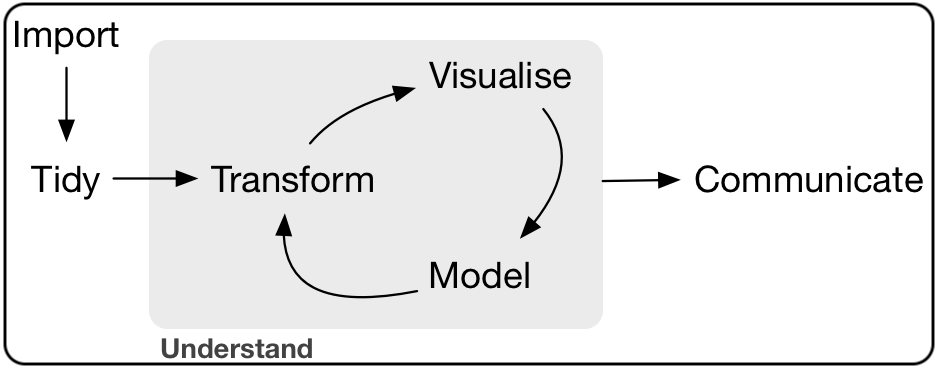
\includegraphics[width=1\linewidth,]{./figures/data_analysis_workflow} 

}

\caption{Data analysis workflow \autocite{wickham_r_2017}. This work focuses primary on multivariate data visualization, but also facilitates transforming data and interpretation of models.}\label{fig:dataanalysisworkflow}
\end{figure}

Early attempts at high-dimension visuals in scatterplot matrices \autocite{chambers_graphical_1983} and parallel coordinate plots\autocite{ocagne_coordonnees_1885}. Pricipal component analysis (PCA, \textcite{pearson_liii._1901}) reorients the basis to components, linear combinations of the original variables ordered by descending amount of variation explained. These components are typically viewed as discrete orthogonal pairs.

A data visualization \emph{tour} \autocite{cook_grand_2008,lee_review_2021} is a class of linear projections that animate small changes to the projection basis. Intuitively, they show a projection of the data object down to lower-dimensional space, in the same way that a 3D object casts a 2D shadow. A key feature of the tour is the persistence and tractability of the points through many frames. In the shadow analogy an object, such as a barstool may be casting a circular shadow that could come from any number of shapes. However, if the stool were rotated the legs would show in the shadow quickly giving an intuitive interpretation of the object. Similarly looking at a data object over the rotation of its variables yields information about its structure. In this way and aided with linked brushing and other interactions, such continuous tours excel at extending the interpretability of multivariate spaces. Chapter \ref{ch:motivation} motivates why we decide to use such linear dimension reduction techniques.

Component spaces, and tours optimize for the certain objectives or choose randomly, though lends itself particularly well \emph{human-in-the-loop} \autocite{karwowski_international_2006} analysis. If the analyst wants to explore what what happens to the structure of one variable were removed or increase the contribution of another. This sort of variable level control is just not possible. The work in \textcite{cook_manual_1997} suggests a means for performing this manipulation though there is no compiling implementaiton of this method.

\hypertarget{research-questions}{%
\section{Research questions}\label{research-questions}}

The over-arching question of interest can be stated as:

\textbf{Can the radial tour with user interaction help analysts understand linear projections, and explore the sensitivity of structure in the projection to the variables contributing to the projection?}

Understanding variable sensitivity to the structure in a projection frame is crucial factor analysis after identifying a feature of interest. If an identified feature is the \emph{what} of an analysis then its variable attributions are its \emph{how}. The user interaction afforded by the radial tour should allow for a more precise exploration of this structure.

RQ 1. \textbf{How do we define user interaction for the radial tours to add and remove variables smoothly from a 2D linear projection of data?}\\
Niether component spaces nor grand tour provide a means for changing the contributions of a desired variable. In order to facilitate variable interaction we need to have a means of manipulating the basis. This crutial to exploring sensitivity of the variable contributions to the structure in a frame.

RQ 2. \textbf{Do analysts understand the relationship between variables and structure in a 2D linear projection better when the radial tour is available?}\\
How can we be certain the having this control leads to a meaningfully method than looking at discrete components or by watching enough continuous frames of grand tour?

RQ 3. \textbf{Can the radial tours be used in conjunction with the local explanation, SHAP, to improve the interpretability of black-box models?}\\
The tension from the trade-off between accuracy and interpretability of black-box models is rising. There is a clear need to be able to explain black-box models. After extaploating local explanations of all observations we want to explore that space with the help of the radial tour.

\hypertarget{methodology}{%
\section{Methodology}\label{methodology}}

The research corresponding with RO \#1 entails \emph{algorithm/software design} adapting the algorithm from \textcite{cook_manual_1997}. This allows for interactive control of 2D projections and serves as a foundation for the remaining work to follow.

To address RO \#2, a controlled \emph{experimental study} has explored the efficacy of interactive radial tours as compared with 2 benchmark methods: Principal Component Analysis (PCA, \textcite{pearson_liii._1901}) and the grand tour \autocite{asimov_grand_1985}. This was a within-participant user study where each participant experienced each visual. Trials were balanced across 3 other experimental factors: location of the signal, the shape of the cluster distributions, and the dimensionality of the data. Ethics approval was obtained for this work. The approval and disclosure form are available at the project repository: \url{https://github.com/nspyrison/spinifex_study/tree/master/ethics}.

The research for RO \#3 involves \emph{fundamental visualization design}. We know that the SAHP value is a local explanation for one observation. This SHAP value will also serve as the 1D basis for the radial tour. While using SHAP as a projection basis is novel it is not particularly insightful by itself. We provide tracking marks on the tour as well as showing the within-class distributions of the SHAP components as parallel coordinate marks on the basis. We also offer a global view and related statistics to map to color to aid in exploring the sensitivity of the SHAP-space relative to the sensitivity of the original data space.

\hypertarget{contributions}{%
\section{Contributions}\label{contributions}}

\begin{enumerate}
\def\labelenumi{\arabic{enumi}.}
\tightlist
\item
  \textbf{spinifex} a package offering a consistent framework for performing radial tour and rendering all tours to various formats:

  \begin{itemize}
  \tightlist
  \item
    Perform radial tours to explore the variable sensitivity to structure
  \item
    Transform numeric variable in the data
  \item
    Extract various bases exposing features of the data
  \item
    Interoperable with tours generated with \textbf{tour} \autocite{wickham_tourr:_2011}
  \item
    Layered interface for producing tours that mirror the layered approach of \textbf{ggplot2} \autocite{wickham_ggplot2_2016}
  \end{itemize}
\item
  A user study comparing the efficacy of the radial tour against the alternatives of PCA the grand tour includes:

  \begin{itemize}
  \tightlist
  \item
    Creation of supervised classification task to assess the variable attribution to the separation of clusters performed under various levels of experimental factors: location, shape, and dimensionality.
  \item
    Definition of an accuracy measure to evaluate this task.
  \item
    Results: strong evidence that the radial tour increases the accuracy of this task by a large amount while the task is performed fastest with the grand tour.
  \item
    Attribution of the error, by performing a mixed model regression helps to explain the source of the error term into the variability of participants skill aptitude for this task and variability of the difficultly of a simulation by random chance.
  \item
    Introduces an interactive application to preprocess data and explore with radial tour. Users can choose from six supplied datasets or upload their own.
  \end{itemize}
\item
  \textbf{cheem} a package applying the radial tour to local explanations of black-box models, including:

  \begin{itemize}
  \tightlist
  \item
    Preproccing; creation of a random forest model, the extraction of all observation's tree SHAP local explanation, and extraction of other statistics for display.
  \item
    Visualization of approximations of the data- and attribution-space side-by-side with linked brushing, hover tooltips, and tabular display of selected points.
  \item
    Evaluating the local explanations with the use of the radial tour we can explore the sensitivity to the structure identified better see what variable support the explanation holds realistic.
  \end{itemize}
\end{enumerate}

\hypertarget{thesis-structure}{%
\section{Thesis structure}\label{thesis-structure}}

The remainder of the thesis is organized as follows: Chapter \ref{ch:motivation} covers the motivation for such research. The research chapters 3 through 5 will cover their respective own backgrounds and follow-up discussion. Chapter \ref{ch:efficacy_radial_tour} discusses a user study evaluating the efficacy of the radial, manual tour. Chapter \ref{ch:cheem} extends the use of manual tours to extend the interpretability of black-box models. Lastly, Chapter \ref{ch:conclusion} concludes with some takeaways and a discussion of possible extensions.

\hypertarget{ch:motivation}{%
\chapter{Motivation}\label{ch:motivation}}

First I motivation the early are frequent us of data visualization in general. Then we discuss some of the alternative data visualizations, and their scalability. The we discuss dimension reduction before cover tours in more detail.

For our purposes I will be focusing the case where data \(X_{nxp}\) contains \(n\) observations of \(p\) variables, is complete with no missing values, variables are numeric (ideally not ordinal levels), and \(n>p\) typically many more observations than variables. While I write as though always operating on the original variable space these methods could similarly be applied to feature decomposition of data not fitting this description. In the case of the linear projection let, \(Y_{nxd} = X_{nxp} * A_{pxd}\) be the embedding of the data mapped by the basis \(A\), where \(d<p\). When \(p\) is large, say over 10 or 20 variables, the viewing space is quite large. In these cases a PCA initialization step is commonly used where the variables are approximated as fewer principal components and this reduced space can be view, albeit with the disadvantage of having another linear mapping back to the original space. \textcite{wickham_visualizing_2015} also views model spaces and features while urging to have a preference for visualizing data-space directly.

Visualization is much more robust than numerical summarization alone \autocite{anscombe_graphs_1973,matejka_same_2017}. In these studies the data have the same summary statistics, yet contains obvious visual trends and shapes that could go completely unheeded if plotting is foregone. Data visualization is fundamental to EDA and quickly evaluating data supports ensuring that models are suitable.



\begin{figure}

{\centering 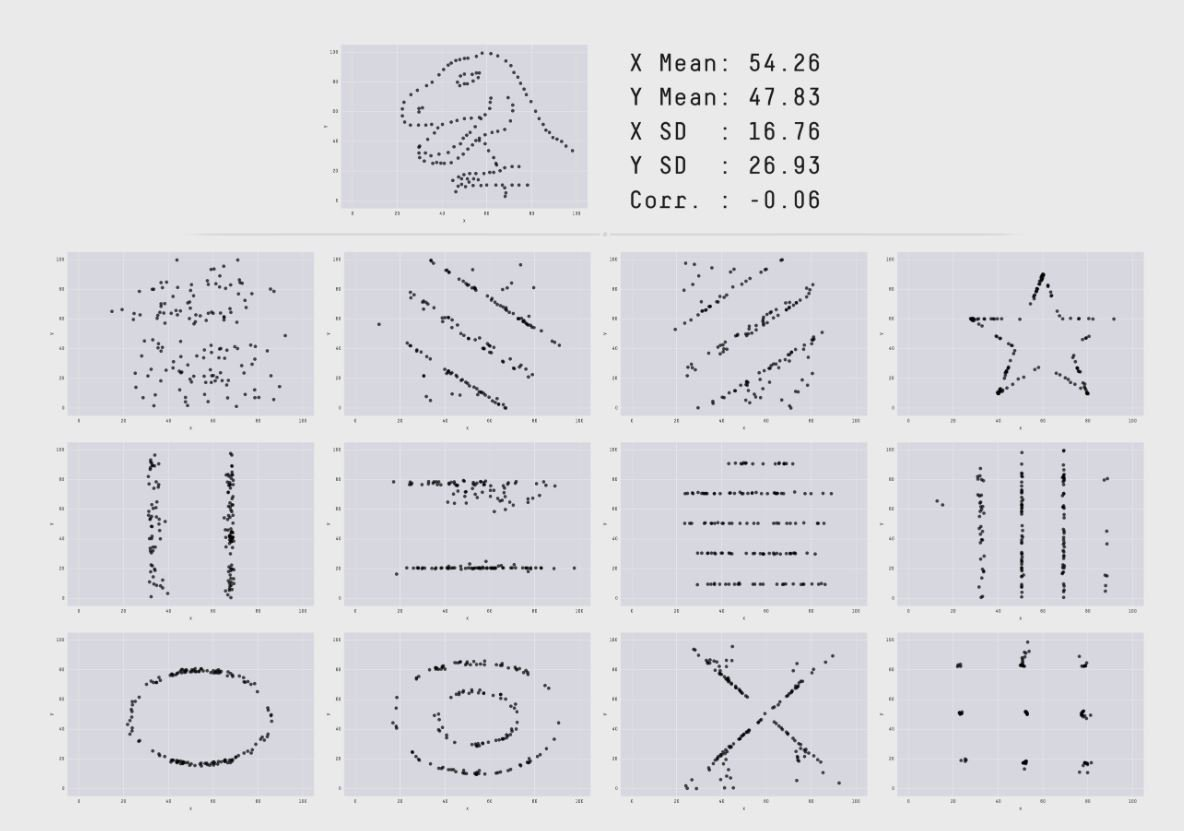
\includegraphics[width=0.7\linewidth,]{./figures/matejka17fig} 

}

\caption{Starting with the datasarus plot, observations are allows to drift (by iterated simulated annealing) toward 12 patterns provided that they stay close to the originally listed statistics \autocite{matejka_same_2017}.}\label{fig:matejka17fig}
\end{figure}

\hypertarget{visualizing-multivariate-data.}{%
\section{Visualizing multivariate data.}\label{visualizing-multivariate-data.}}

The work in \textcite{grinstein_high-dimensional_2002} gives a good taxonomy of high-dimensional visualization. We will follow a few examples building up to why we conclude with tour methods. Broadly speaking, we are concerned with the question ``How can an analyst visualize arbitrary \(p-\) dimensions?''. To illustrate some of the options for data I use the penguins data\autocite[horst\_palmerpenguins\_2020]{gorman_ecological_2014}. It contains 333 observations of 4 physical measurements for 3 species of penguins observed near Palm Station, Antarctica.

Viewing as many univariate histograms or density curves is one method. Similarly, one could look at all variable pairing as scatter plots. This forms the crux of scatterplot matrices, also known as SPLOM \autocite{chambers_graphical_1983}. In a scatterplot matrix variables are displayed across the columns and row, the diagonal elements show the univariate densities while one or both sides of the off diagonal show scatterplot pairs. This is useful for getting a handle on the support and shapes of the variables, but is not going to scale well with dimension and is not a suitable audience-ready display as it is very busy and doesn't draw attention to any one spot. Munzner reminds us to abstract all of the cognitive work out of the visual allowing the audience to focus on seeing the evidence supporting the claim \autocite{munzner_visualization_2014}.



\begin{figure}

{\centering 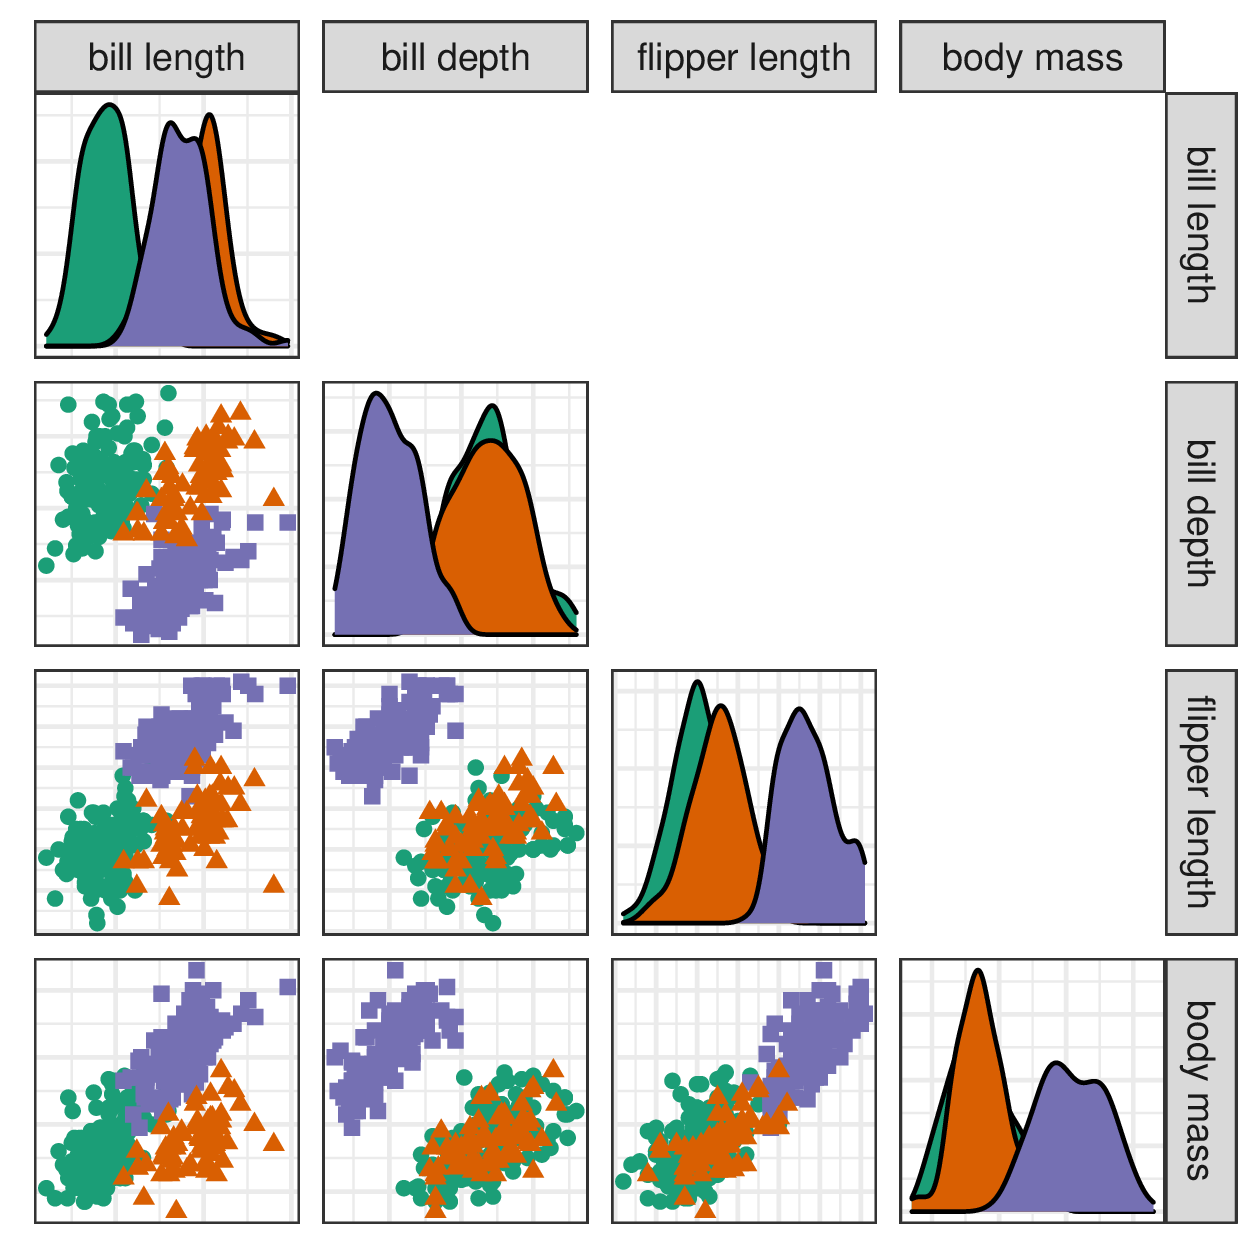
\includegraphics[width=1\linewidth,]{./figures_from_script/ch2_fig1_penguin_splom} 

}

\caption{(ref:penguinsmplom-cap)}\label{fig:penguinsplom}
\end{figure}

Alternatively, we could consider a class of observation-based visuals. In parallel coordinate plots \autocite{ocagne_coordonnees_1885} variables are arranged horizontally and observations are connected by lines with the height mapping to the quantile or z-value for each variable. This scales much better with dimensions, but poorly with observations. It also suffers from an asymmetry with the variable order, that is, changing the order of the variable will lead people to very different conclusions. The x-axis is also used to display variables rather than the values of the observations. This restricts the amount of information that can be gleaned between variables. Munzner asserts that position is the more human-perceptible channel for encoding information; we should like to reserve it for the values of the observations. The same issues persist across other observation-based displays such as radial variants, pixel-oriented visuals, and Chernoff faces {[}\textcite{keim_designing_2000}; chernoff\_use\_1973{]}. These visuals are better suited for the \(n<p\) case where there are more variables than observations.



\begin{figure}

{\centering 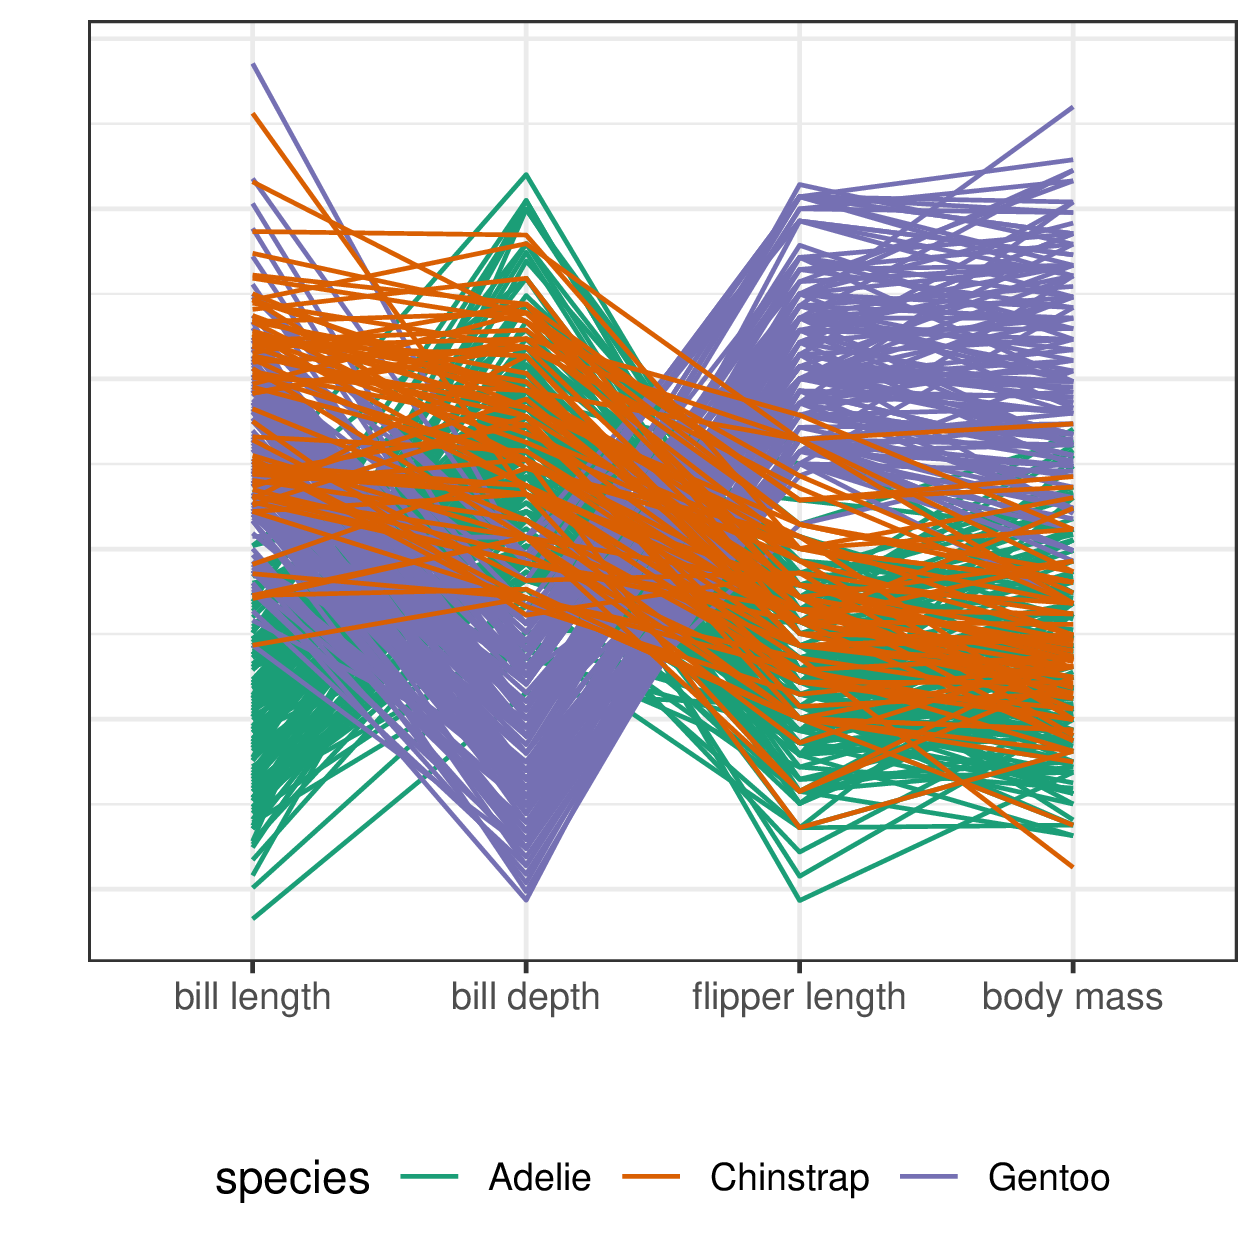
\includegraphics[width=1\linewidth,]{./figures_from_script/ch2_fig2_penguin_pcp} 

}

\caption{Parallel coordinate plots of penguins data. Doesn't scale well with observations, suffers from asymmetry with the variable ordering, and horizontal position is used for variable rather than observation levels.}\label{fig:penguinpcp}
\end{figure}

\hypertarget{dimension-reduction}{%
\section{Dimension reduction}\label{dimension-reduction}}

Ultimately, we will need to turn to dimension reduction to create a compelling visual allowing audiences to focus on features with contributions from multiple variables. Dimension reduction is separated into two categories, linear and non-linear. The linear case spans all affine mathematical transformations, essentially any mapping where parallel lines stay parallel. Non-linear transformations are the complement of that, think transformations with exponents or interacting terms. Examples in low dimension are relatable. For instance shadows are examples of linear projections where a 3-dimensional object casts a 2D projection, the shadow. Our vision at one instance in time is also a 2D projection-perspective. An example of a non-linear transformation is that of 2D representation of the globe. There are many different ways (and features to optimize) to distort the surface to display as a map. Most common may be rectangular display where area is distorted more and more with distance away from the equator. Other distortions are created when the surface is unwrapped as a long ellipse. Yet others create non-continuous gaps in oceans to minimize the distortion of countries.

Non-linear techniques often have hyperparameters that affect how the spaces are distorted to fit into a lower-space. To quote Anastasios Panagiotelis ``All non-linear projections are wrong, but some are useful'', a play on George Box quote about models. Non-linear techniques distort the space in unclear ways, and what is more, they can introduce features not in the data depending on the selection of hyperparameters. It feels like they are necessary, but not sufficient to conclude the existence of a feature, that is, if a non-linear embedding resolves a feature, we shouldn't be certain that it really exists in the data.

Unfortunately, there is no free lunch here. An increase in data space will lead a \(p-d\)-dimensional viewing space in the linear case and an increasingly perturbed and distorted space in non-linear techniques. The intrinsic dimensionality of data is the number of variables needed to minimally represent the data \autocite{grinstein_high-dimensional_2002}. This is an important aspect of dimension reduction that does not have to end in visual, but is also a common part of factor analysis and preprocessing data. Consider a Psychology survey consisting of 100 questions about the Big Five personality traits. The data consists of 100 variables, while the theory would suggest the intrinsic dimensionality is five. The data likely picks up on other aspects and may better be summarized in with 8 or 10 dimensions. If this were the case, reducing the data to this space will be necessary to gate the exponentially increasing view time.

\hypertarget{tours-animated-linear-projections}{%
\section{Tours, animated linear projections}\label{tours-animated-linear-projections}}

A single linear projection is a resulting space from the data multiplied by the basis where the basis is an orthonormal matrix (the orientation of the unit origin) mapping the data space to a lower dimension. A data visualization tour animates many such projections through small changes in the basis. Originally in a \emph{grand} tour \autocite{asimov_grand_1985} several target frames are randomly selected and then interpolated along their geodesic path.



\begin{figure}

{\centering 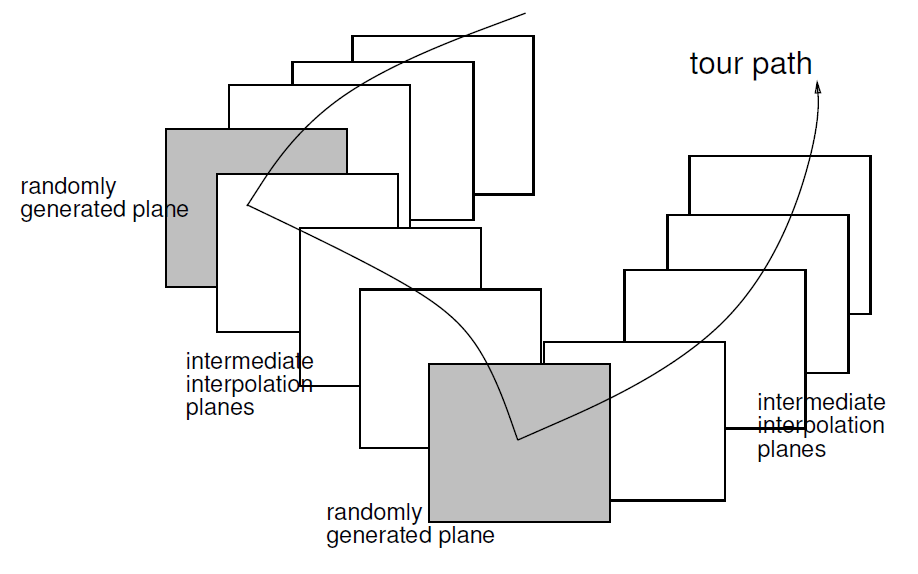
\includegraphics[width=1\linewidth,]{./figures/buja05fig} 

}

\caption{Illustration of the grand tour selecting random target frames (grey) connected via geodesically interpolated frame (white), figure from \textcite{buja_computational_2005}.}\label{fig:buja05fig}
\end{figure}

There are various types of tours that are classified by the generation of their basis paths. A \emph{guided} tour uses simulated annealing to move progressively closer to an objective function in the embedded space\autocite{hurley_analyzing_1990}. A more comprehensive discussion and review of tours can be found in the works of \textcite{cook_grand_2008}; \textcite{lee_review_2021}{]}.

Tours are used for a couple of salient features: maintains transparency back to the original variable space and the persistence data points from frame to frame convey more information than looking at discrete jumps to other bases. Because of these features tours are a good method to extend the visualization of data space as dimensionality increases.

The work below covers manual tours \autocite{cook_manual_1997,spyrison_spinifex_2020} in Chapter \ref{ch:spinifex}. Radial tours are one type of manual tour that where the contribution of one variable is extended radially to a full contribution, removed completely, then restored to its original contribution. Chapter \ref{ch:efficacy_radial_tour} compares the efficacy of the radial tour as compared with PCA and the grand tour in a user study. Lastly, Chapter \ref{ch:cheem} extends the use of the radial tour to evaluate the local explanation of black-box models.

\hypertarget{ch:spinifex}{%
\chapter{spinifex: An R Package for Creating a Manual Tour of Low-dimensional Projections of Multivariate Data}\label{ch:spinifex}}

TODO:XXX Segue. Bring over abstract?

\hypertarget{introduction}{%
\section{Introduction}\label{introduction}}

Exploring multivariate spaces is a challenging task, increasingly so as dimensionality increases. Traditionally, static low-dimensional projections are used to display multivariate data in two dimensions including principal component analysis, linear discriminant spaces or projection pursuit. These are useful for finding relationships between multiple variables, but they are limited because they show only a glimpse of the high-dimensional space. An alternative approach is to use a tour \autocite{asimov_grand_1985} of dynamic linear projections to look at many different low-dimensional projections. Tours can be considered to extend the dimensionality of visualization, which is important as data and models exist in more than 3D. The package \{tourr\} \autocite{wickham_tourr:_2011} provides a platform for generating tours. It can produce a variety of tours, each paired with a variety of possible displays. A user can make a grand, guided, little, local or frozen tour, and display the resulting projected data as a scatterplot, density plot, histogram, or even as Chernoff faces if the projection dimension is more than 3.

This work adds a manual tour to the collection. The manual tour was described in \textcite{cook_manual_1997} and allows a user to control the projection coefficients of a selected variable in a 2D projection. The manipulation of these coefficients allows the analyst to explore their sensitivity to the structure within the projection. As manual tours operate on only one variable at a time, they are particularly useful once a feature of interest has been identified.

One way to identify ``interesting'' features is with the use of a guided tour \autocite{cook_grand_1995}. Guided tours select a very specific path, which approaches a projection that optimizes an objective function. The optimization used to guide the tour is simulated annealing \autocite{kirkpatrick_optimization_1983}. The direct optimization of a function allows guided tours to rapidly identify interesting projection features given the relatively large parameter-space. After a projection of interest is identified, an analyst can then use the ``finer brush'' of the manual tour to control the contributions of individual variables to explore the sensitivity they have on the structure visible in the projection.

The paper is organized as follows. Section \ref{sec:algorithm} describes the algorithm used to perform a radial manual tour as implemented in the package \{spinifex\}. Section \ref{sec:display} explains how to generate an animation of the manual tour using the animation frameworks offered by \{plotly\} \autocite{sievert_interactive_2020} and \{gganimate\} \autocite{pedersen_gganimate_2020}. Package functionality and code usage following the order applied in the algorithm follows in section \ref{sec:usage}. Section \ref{sec:application} illustrates how this can be used for sensitivity analysis applied to multivariate data collected on high energy physics experiments \autocite{wang_mapping_2018}. Section \ref{sec:discussion} summarizes this paper and discusses potential future directions.

\hypertarget{sec:algorithm}{%
\section{Algorithm}\label{sec:algorithm}}

The algorithm to conduct a manual tour interactively, by recording mouse/cursor motion, is described in detail in \textcite{cook_manual_1997}. Movement can be in any direction and magnitude, but it can also be constrained in several ways:

\begin{itemize}
\tightlist
\item
  \emph{radial}: fix the direction of contribution, and allow the magnitude to change.
\item
  \emph{angular}: fix the magnitude, and allow the angle or direction of the contribution to vary.
\item
  \emph{horizontal}, \emph{vertical}: allow rotation only around the horizontal or vertical axis of the current 2D projection.
\end{itemize}

The algorithm described here produces a \textbf{radial} tour as an \emph{animation sequence}. It takes the current contribution of the chosen variable, and using rotation brings this variable fully into the projection, completely removes it, and then returns to the original position.

\hypertarget{notation}{%
\subsection{Notation}\label{notation}}

The notation used to describe the algorithm for a 2D radial manual tour is as follows:

\begin{itemize}
\item
  \(\textbf{X}\), the data, an \(n \times p\) numeric matrix to be projected to 2D.
\item
  \(\textbf{B} = (B_1,~ B_2)\), any 2D orthonormal projection basis, \(p \times 2\) matrix, describing the projection from \(\mathbb{R}^p \Rightarrow \mathbb{R}^2\). This is called this the ``original projection'' because it is the starting point for the manual tour.
\item
  \(k\), is the index of the variable to manipulate, called the ``manip var''.
\item
  \(\textbf{e}\), a 1D basis vector of length \(p\), with 1 in the \(k\)-th position and 0 elsewhere.
\item
  \(\textbf{M}\) is a \(p \times 3\) matrix, defining the 3D subspace where data rotation occurs and is called the manip(ulation) space.
\item
  \(\textbf{R}\), the 3D rotation matrix, for performing unconstrained 3D rotations within the manip space, \(\textbf{M}\).
\item
  \(\theta\), the angle of in-projection rotation, for example, on the reference axes; \(c_\theta, s_\theta\) are its cosine and sine.
\item
  \(\phi\), the angle of out-of-projection rotation, into the manip space; \(c_\phi, s_\phi\) are its cosine and sine. The initial value for animation purposes is \(\phi_1\).
\item
  \(\textbf{U}\), the axis of rotation for out-of-projection rotation orthogonal to \(\textbf{e}\).
\item
  \(\textbf{Y}\), the resulting projection of the data through the manip space, \(\textbf{M}\), and rotation matrix, \(\textbf{R}\).
\end{itemize}

The algorithm operates entirely on projection bases and incorporates the data only when making the projected data plots, in light of efficiency.

\hypertarget{steps}{%
\subsection{Steps}\label{steps}}

\hypertarget{step-0-setup}{%
\subsubsection{Step 0) Setup}\label{step-0-setup}}

The flea data (\textcite{lubischew_use_1962}), available in the \{tourr\} package, is used to illustrate the algorithm. The data contains 74 observations on 6 variables, which are physical measurements made on flea beetles. Each observation belongs to one of three species.

An initial 2D projection basis must be provided. A suggested way to start is to identify an interesting projection using a projection pursuit guided tour. Here the holes index is used to find a 2D projection of the flea data, which shows three separated species groups. Figure \ref{fig:ch3fig1} shows the initial projection of the data. The left panel displays the projection basis (\(\textbf{B}\)) and can be used as a visual guide of the magnitude and direction that each variable contributes to the projection. The right panel shows the projected data, \(\textbf{Y}_{[n,~2]} ~=~ \textbf{X}_{[n,~p]} \textbf{B}_{[p,~2]}\). The color and shape of points are mapped to the flea species. This plot is made using the \texttt{view\textbackslash{}\_basis()} function in \{spinifex\}, which generates a \{ggplot2\} \autocite{wickham_ggplot2_2016} object.

\begin{figure}

{\centering 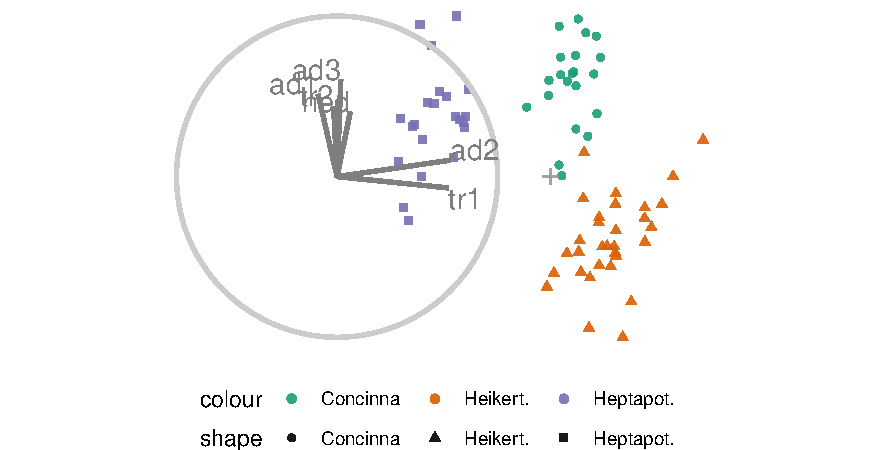
\includegraphics[width=1\linewidth,]{./figures_from_script/ch3_fig1_biplot} 

}

\caption{Biplot of the initial 2D projection: representation of the basis (left) and resulting data projection (right) of standardized flea data. The color and shape of data points are mapped to the species of flea beetle. The basis was produced by a projection pursuit guided tour, with the holes index. The contribution of the variables aede2 and tars1 approximately contrasts the other variables. The visible structure in the projection are the three clusters corresponding to the three species.}\label{fig:ch3fig1}
\end{figure}

\hypertarget{step-1-choose-manip-variable}{%
\subsubsection{Step 1) Choose manip variable}\label{step-1-choose-manip-variable}}

In figure \ref{fig:ch3fig1} the contribution of the variables tars1 and aede2 mostly contrast the contribution of the other four variables. These two variables combined contribute in the direction of the projection where the purple cluster is separated from the other two clusters. The variable aede2 is selected as the manip var, the variable to be controlled in the tour. The question that will be explored is: how important is this variable to the separation of the clusters in this projection?

\hypertarget{step-2-create-the-3d-manip-space}{%
\subsubsection{Step 2) Create the 3D manip space}\label{step-2-create-the-3d-manip-space}}

Initialize the coordinate basis vector as a zero vector, \(\textbf{e}\), of length \(p\), and set the \(k\)-th element to 1. In the example data, aede2 is the fifth variable in the data, so \(k=5\), set \(e_5=1\). Use a Gram-Schmidt process to orthonormalize the coordinate basis vector on the original 2D projection to describe a 3D manip space, \(\textbf{M}\).

\begin{align*}
  e_k &\leftarrow 1 \\ 
  \textbf{e}^*_{[p,~1]} &= \textbf{e} - \langle \textbf{e}, \textbf{B}_1 \rangle \textbf{B}_1 - \langle \textbf{e}, \textbf{B}_2 \rangle \textbf{B}_2 \\ 
  \textbf{M}_{[p,~3]} &= (\textbf{B}_1,\textbf{B}_2,\textbf{e}^*)
\end{align*}

The manip space provides a 3D projection from \(p\)-dimensional space, where the coefficient of the manip var can range completely between {[}0, 1{]}. This 3D space serves as the medium to rotate the projection basis relative to the selected manipulation variable. Figure \ref{fig:ch3fig2} illustrates this 3D manip space with the manip var highlighted. This representation is produced by calling the \texttt{view\textbackslash{}\_manip\textbackslash{}\_space()} function. This diagram is purely used to help explain the algorithm.

\begin{figure}

{\centering 
\includegraphics[width=1\linewidth,]{./figures_from_script/ch3_fig2_manip_sp} 

}

\caption{Illustration of a 3D manip space, the projection plane is shown as blue circle extending into and out of the display. A manipulation direction is initalized, the red circle, orthogonal to the projection plane. This allows the selected variable, aede2, a means to change it's contribution back to the projection plane. The other variables contributions rotate into this space as well, preserving the orthagonal structure, but are omitted in the manipulation dimension for simplicity.}\label{fig:ch3fig2}
\end{figure}

\hypertarget{step-3-defining-a-3d-rotation}{%
\subsubsection{Step 3) Defining a 3D rotation}\label{step-3-defining-a-3d-rotation}}

The basis vector corresponding to the manip var (red line in Figure \ref{fig:ch3fig2}), can be operated like a lever anchored to the origin. This is the process of the manual control, that rotates the manip variable into and out of the 2D projection (Figure \ref{fig:ch3fig3}). As the variable contribution is controlled, the manip space rotates, and the projection onto the horizontal projection plane correspondingly changes. This is a manual tour. Generating a sequence of values for the rotation angles produces a path for the rotation of the manip space.

For a radial tour, fix \(\theta\), the angle describing rotation within the projection plane, and compute a sequence for \(\phi\), defining movement out of the plane. This will change \(\phi\) from the initial value, \(\phi_1\), the angle between \(\textbf{e}\) and its shadow in \(\textbf{B}\), to a maximum of \(0\) (manip var fully in projection), then to a minimum of \(\pi/2\) (manip var out of projection), before returning to \(\phi_1\).

Rotations in 3D can be defined by the axes they pivot on. Rotation within the projection, \(\theta\), is rotation around the \(Z\) axis. Out-of-projection rotation, \(\phi\), is the rotation around an axis on the \(XY\) plane, \(\textbf{U}\), orthogonal to \(\textbf{e}\). Given these axes, the rotation matrix, \(\textbf{R}\) can be written as follows, using Rodrigues' rotation formula (originally published in \textcite{rodrigues_lois_1840}):

\begin{align*}
    \textbf{R}_{[3,~3]} 
    &= \textbf{I}_3 + s_\phi\*\textbf{U} + (1-c_\phi)\*\textbf{U}^2 \\
        &=
    \begin{bmatrix}
      1 & 0 & 0 \\ 
      0 & 1 & 0 \\ 
      0 & 0 & 1 \\
    \end{bmatrix} +
    \begin{bmatrix}
      0 & 0 & c_\theta s_\phi \\
      0 & 0 & s_\theta s_\phi \\
      -c_\theta s_\phi & -s_\theta s_\phi & 0 \\
    \end{bmatrix} +
    \begin{bmatrix}
      -c_\theta (1-c_\phi) & s^2_\theta (1-c_\phi) & 0 \\
      -c_\theta s_\theta (1-c_\phi) & -s^2_\theta (1-c_\phi) & 0 \\
      0 & 0 & c_\phi-1 \\
    \end{bmatrix} \\
    &= 
    \begin{bmatrix}
      c_\theta^2 c_\phi + s_\theta^2 &
      -c_\theta s_\theta (1 - c_\phi) &
      -c_\theta s_\phi \\
      -c_\theta s_\theta (1 - c_\phi) &
      s_\theta^2 c_\phi + c_\theta^2 &
      -s_\theta s_\phi \\
      c_\theta s_\phi &
      s_\theta s_\phi &
      c_\phi
    \end{bmatrix} \\
\end{align*}

\noindent where

\begin{align*}
  \textbf{U} &= (u_x, u_y, u_z) =
  (s_\theta, -c_\theta, 0) \\ 
  &=
  \begin{bmatrix}
  0 & -u_z & u_y  \\
  u_z & 0 & -u_x \\
  -u_y & u_x & 0 \\
  \end{bmatrix} =
  \begin{bmatrix}
    0 & 0 & -c_\theta \\
    0 & 0 & -s_\theta \\
    c_\theta & s_\theta & 0 \\
  \end{bmatrix} \\
  \end{align*}

\hypertarget{step-4-creating-an-animation-of-the-radial-rotation}{%
\subsubsection{Step 4) Creating an animation of the radial rotation}\label{step-4-creating-an-animation-of-the-radial-rotation}}

The steps outlined above can be used to create any arbitrary rotation in the manip space. To use these for sensitivity analysis, the radial rotation is built into an animation where the manip var is rotated fully into the projection, completely out, and then back to the initial value. This involves allowing \(\phi\) to vary between \(0\) and \(\pi/2\), call the steps \(\phi_i\).

\begin{figure}

{\centering 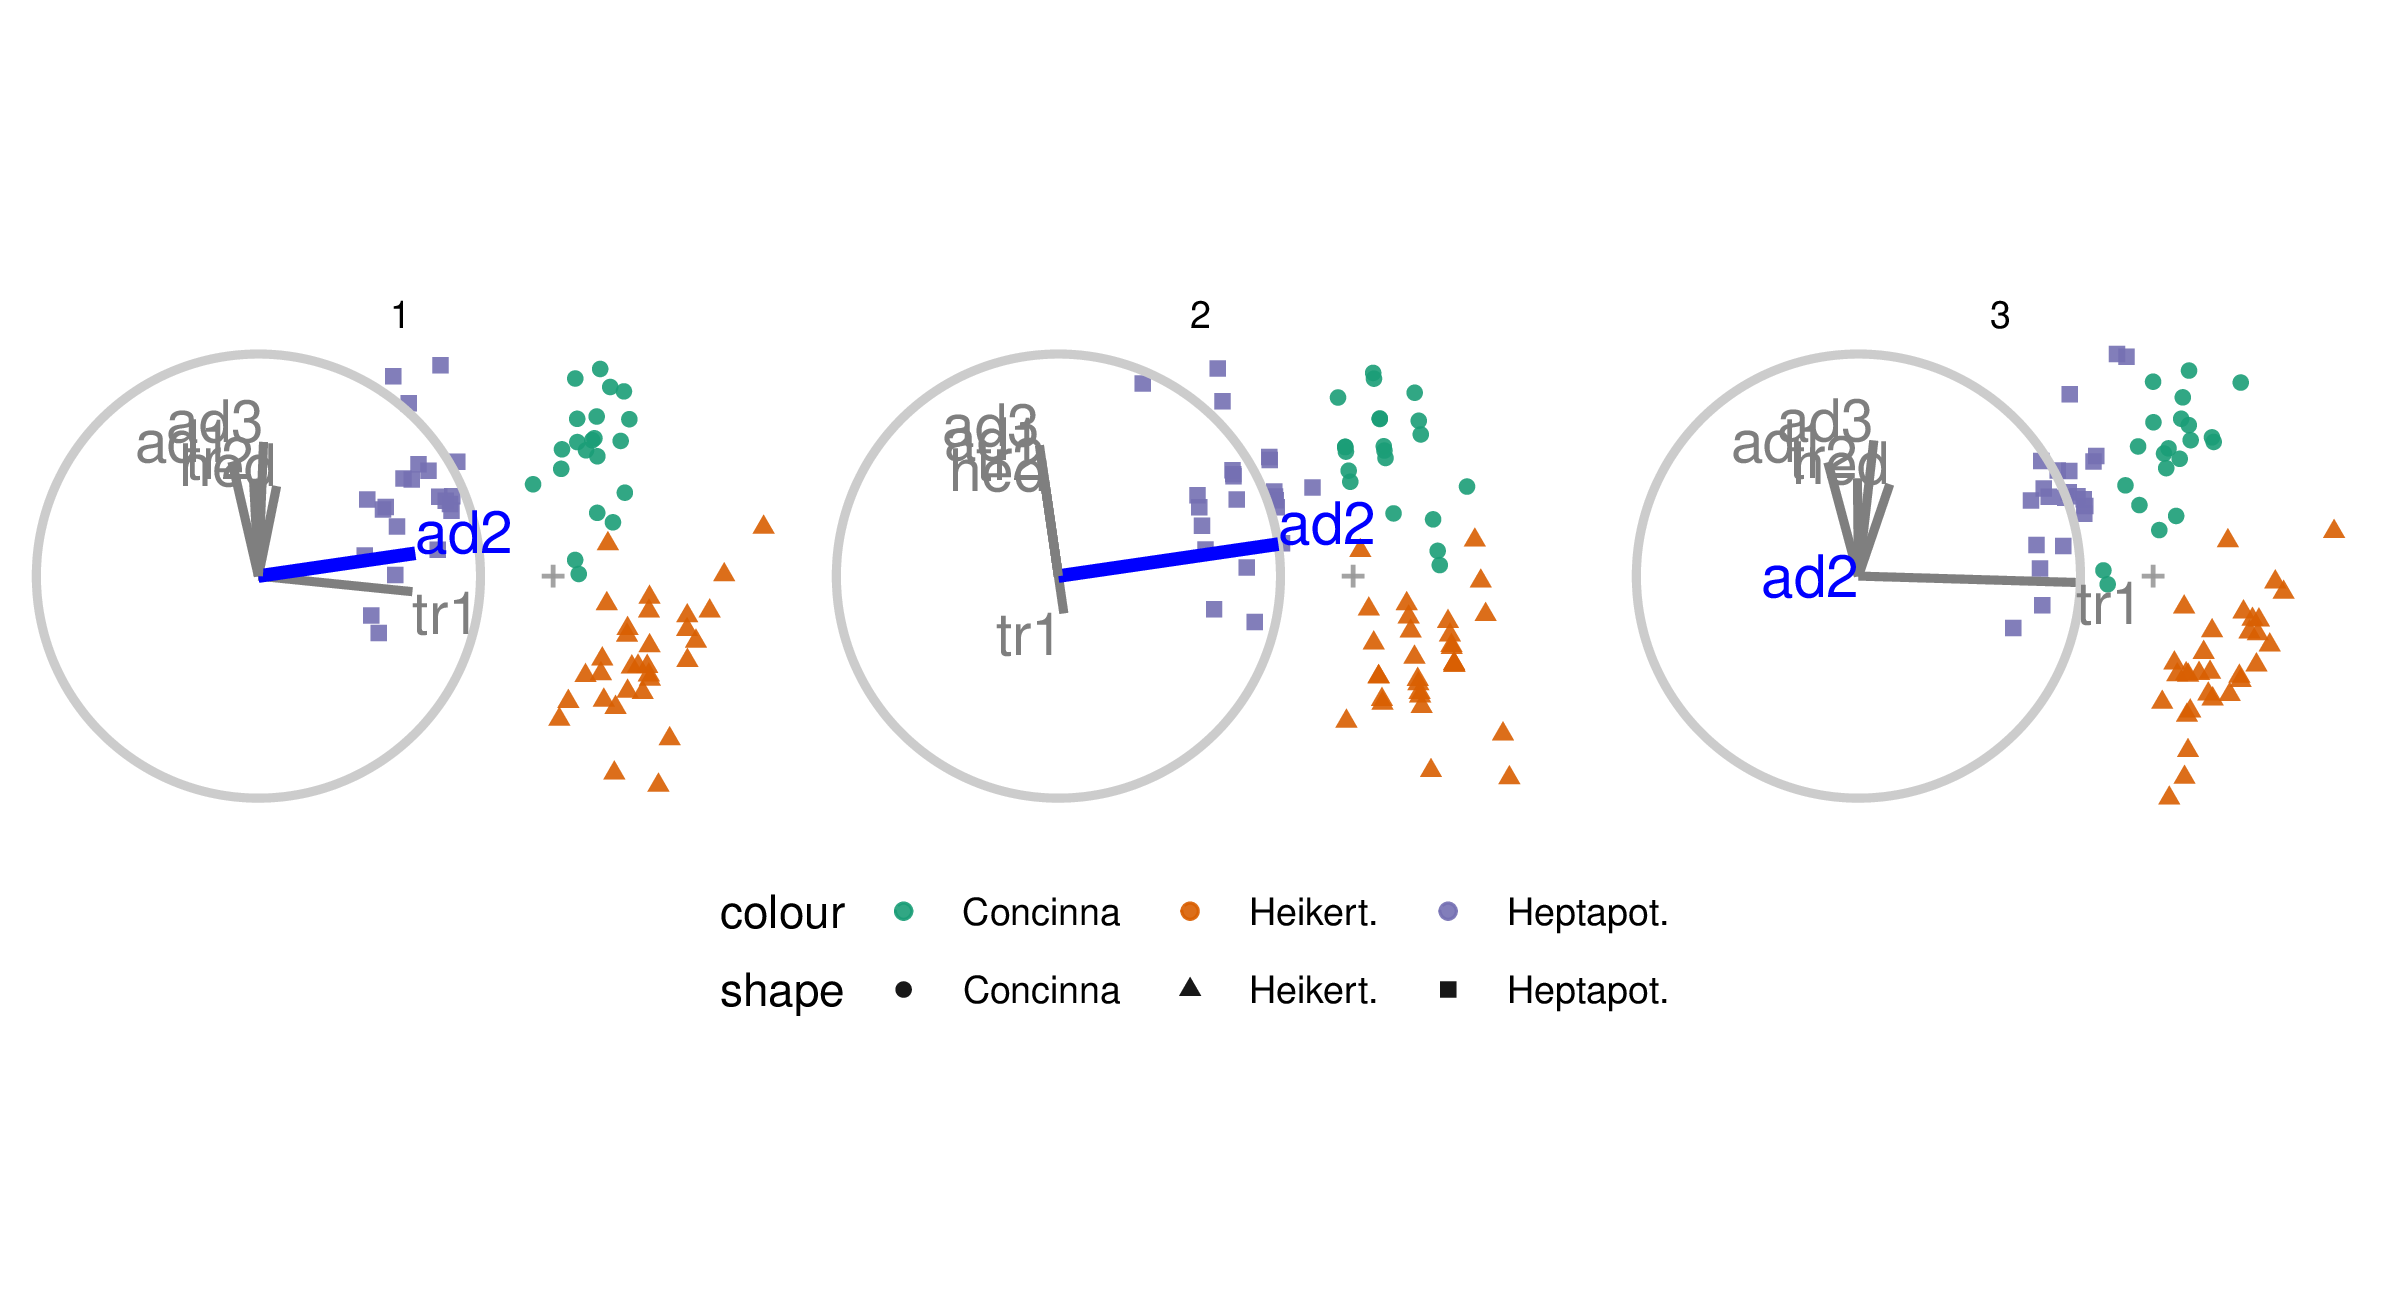
\includegraphics[width=1\linewidth,]{./figures_from_script/ch3_fig3_filmstrip} 

}

\caption{Select frames highlight the animation of a radial manual tour manipulating aede2: (1) original projection, (2) full contribution, (3) zero contribution, before returning to the original original contribution.}\label{fig:ch3fig3}
\end{figure}

\begin{enumerate}
\def\labelenumi{\arabic{enumi}.}
\tightlist
\item
  Set initial value of \(\phi_1\) and \(\theta\): \(\phi_1 = \cos^{-1}{\sqrt{B_{k1}^2+B_{k2}^2}}\), \(\theta = \tan^{-1}\frac{B_{k2}}{B_{k1}}\). Where \(\phi_1\) is the angle between \(\textbf{e}\) and its shadow in \(\textbf{B}\).
\item
  Set an angle increment (\(\Delta_\phi\)) that sets the step size for the animation, to rotate the manip var into and out of the projection. (Note: Using angle increment, rather than a number of steps, to control the movement, is consistent with the tour algorithm as implemented in the \{tourr\}).
\item
  Step towards \(0\), where the manip var is completely in the projection plane.
\item
  Step towards \(\pi/2\), where the manip variable has no contribution to the projection.
\item
  Step back to \(\phi_1\).
\end{enumerate}

In each of the steps 3-5, a small step may be added to ensure that the endpoints of \(\phi\) (\(0\), \(\pi/2\), \(\phi_1\)) are reached.

\hypertarget{sec:display}{%
\subsubsection{Step 5) Projecting the data}\label{sec:display}}

The operation of a manual tour is defined on the projection bases. Only when the data plot needs to be made is the data projected into the relevant basis.

\begin{align*}
  \textbf{Y}^{(i)}_{[n,~3]} &= \textbf{X}_{[n,~p]} \textbf{M}_{[p,~3]} \textbf{R}^{(i)}_{[3,3]}
\end{align*}

\noindent where \(\textbf{R}^{(i)}_{[3,3]}\) is the incremental rotation matrix, using \(\phi_i\). To make the data plot, use the first two columns of \textbf{Y}. Show the projected data for each frame in sequence to form an animation.

Tours are typically viewed as an animation. The animation of this tour can be viewed online at \url{https://github.com/nspyrison/spinifex_paper/blob/master/paper/gifs/flea_radialtour_mvar5.gif}. The page may take a moment to load. Animations can be produced using the function \texttt{play\textbackslash{}\_manual\textbackslash{}\_tour()}.

\hypertarget{package-structure-and-functionality}{%
\section{Package structure and functionality}\label{package-structure-and-functionality}}

This section describes the functions available in the package, and how to use them.

\hypertarget{installation}{%
\subsection{Installation}\label{installation}}

The \{spinifex\} is available from CRAN, and can be installed by:

\begin{Shaded}
\begin{Highlighting}[]
\CommentTok{\# Setup:}
\FunctionTok{install.package}\NormalTok{(}\StringTok{"spinifex"}\NormalTok{) }\DocumentationTok{\#\# Install from CRAN}
\FunctionTok{library}\NormalTok{(}\StringTok{"spinifex"}\NormalTok{) }\DocumentationTok{\#\# Read into session}

\CommentTok{\# Getting started:}
\DocumentationTok{\#\# Shiny app for visualizing basic application}
\FunctionTok{run\_app}\NormalTok{(}\StringTok{"intro"}\NormalTok{)}
\DocumentationTok{\#\# View the code vignette}
\FunctionTok{vignette}\NormalTok{(}\StringTok{"spinifex\_vignette"}\NormalTok{)}
\end{Highlighting}
\end{Shaded}

\hypertarget{functions}{%
\subsection{Functions}\label{functions}}

Table \ref{tab:functionsTable} lists the primary functions and their purpose. These are grouped into four types: construction for building a tour path, render to make the plot objects, animation for running the animation, and specialty for providing illustrations used in the algorithm description.

\begin{table}

\caption{\label{tab:functionsTable}Summary of available functions.}
\centering
\begin{tabular}[t]{lll}
\toprule
Type & Function & Description\\
\midrule
construction & create\_manip\_space & forms the 3D space of rotation\\
construction & rotate\_manip\_space & performs 3D rotation\\
construction & manual\_tour & generates sequence of 2D frames\\
 &  & \\
render & array2df & turn the tour path array into long form, for plotting\\
render & render\_ & render long form as a ggplot2 objection for animation\\
render & render\_plotly & render the animation as a plotly object (default)\\
render & render\_gganimate & render the animation as a gganimate object\\
 &  & \\
animation & play\_tour\_path & composite function animating the specified tour path\\
animation & play\_manual\_tour & composite function animating the specified manual tour\\
 &  & \\
specialty & print\_manip\_space & table of the rotated basis and manip space\\
specialty & oblique\_frame & display the reference axes of a given basis\\
specialty & view\_manip\_space & illustrative display of any manip space\\
\bottomrule
\end{tabular}
\end{table}

\hypertarget{sec:usage}{%
\subsection{Usage}\label{sec:usage}}

Using the flea data from the \{tourr\} package, we will illustrate generating a manual tour to explore the sensitivity of the cluster structure is to the variable aede2.

\noindent The \texttt{play\textbackslash{}\_manual\textbackslash{}\_tour()} function is a composite function handling interaction between \texttt{manual\textbackslash{}\_tour()}, \texttt{array2df()}, and \texttt{render\textbackslash{}\_plotly()}. This will generate an html animation using plotly. Switching the renderer to \texttt{render\textbackslash{}\_gganimate()} alternatively creates an animated gif. Each of these formats allows for the animation to be made available on a web site, or directly visible in an html formatted document.

\hypertarget{making-illustrations}{%
\subsection{Making illustrations}\label{making-illustrations}}

The function \texttt{oblique\_frame} can be used to show a projection of the basis, or with the data overlaid. For example, the plots in Figures \ref{fig:ch3fig1} and \ref{fig:ch3fig3} were made with code similar to this:

\noindent An illustration of the manip space (as shown in Figure \ref{fig:ch3fig2}) is made with the \texttt{view\_manip\_space} function, as follows:

\begin{Shaded}
\begin{Highlighting}[]
\DocumentationTok{\#\# Displays the projection plane and manipulation space for the }
\FunctionTok{view\_manip\_space}\NormalTok{(}\AttributeTok{basis =}\NormalTok{ f\_basis, }
                 \AttributeTok{manip\_var =}\NormalTok{ f\_mvar, }
                 \AttributeTok{lab =} \FunctionTok{colnames}\NormalTok{(f\_data))}
\end{Highlighting}
\end{Shaded}

\hypertarget{sec:application}{%
\section{Application}\label{sec:application}}

\textcite{wang_mapping_2018} introduces a new tool, PDFSense, to visualize the sensitivity of hadronic experiments to nucleon structure. The parameter-space of these experiments lies in 56 dimensions, \(\delta \in \mathbb{R}^{56}\), and are visualized as 3D subspaces of the 10 first principal components in linear (PCA) and non-linear (t-SNE) embeddings.

\textcite{cook_dynamical_2018} illustrates how to learn more about the structures using a grand tour. Tours can better resolve the shape of clusters, intra-cluster detail, and better outlier detection than PDFSense \& TFEP (TensorFlow embedded projections) or traditional static embeddings. This example builds from here, illustrating how the manual tour can be used to examine the sensitivity of structure in a projection to different parameters. The specific 2D projections passed to the manual tour were provided in their work.

The data has a hierarchical structure with top-level clusters; DIS, VBP, and jet. Each cluster is a particular class of experiments, each with many experimental datasets which, each have many observations of their own. In consideration of data density, we conduct manual tours on subsets of the DIS and jet clusters. This explores the sensitivity of the structure to each of the variables in turn and we present the subjectively best and worst variable to manipulate for identifying dimensionality of the clusters and describing the span of the clusters.

\hypertarget{jet-cluster}{%
\subsection{Jet cluster}\label{jet-cluster}}

The jet cluster resides in a smaller dimensionality than the full set of experiments with four principal components explaining 95\% of the variation in the cluster \autocite{cook_dynamical_2018}. The data within this 4D embedding is further subsetted, to ATLAS7old and ATLAS7new, to focus on two groups that occupy different parts of the subspace. Radial manual tours controlling contributions from PC4 and PC3 are shown in Figures \ref{fig:ch3fig4} and \ref{fig:ch3fig5}, respectively. The difference in shape can be interpreted as the experiments probing different phase-spaces. Back-transforming the principal components to the original variables can be done for a more detailed interpretation.

When PC4 is removed from the projection (Figure \ref{fig:ch3fig4}) the difference between the two groups is removed, indicating that it is important for distinguishing experiments. However, removing PC3 from the projection (Figure \ref{fig:ch3fig5}) does not affect the structure, indicating it is not important for distinguishing experiments. Animations for the remaining PCs can be viewed at the following links: \href{https://github.com/nspyrison/spinifex_paper/blob/master/paper/gifs/jetcluster_manualtour_pc1.gif}{PC1}, \href{https://github.com/nspyrison/spinifex_paper/blob/master/paper/gifs/jetcluster_manualtour_pc2.gif}{PC2}, \href{https://github.com/nspyrison/spinifex_paper/blob/master/paper/gifs/jetcluster_manualtour_pc3.gif}{PC3}, and \href{https://github.com/nspyrison/spinifex_paper/blob/master/paper/gifs/jetcluster_manualtour_pc4.gif}{PC4}. It can be seen that only PC4 is important for viewing the difference in these two experiments.

\begin{figure}

{\centering 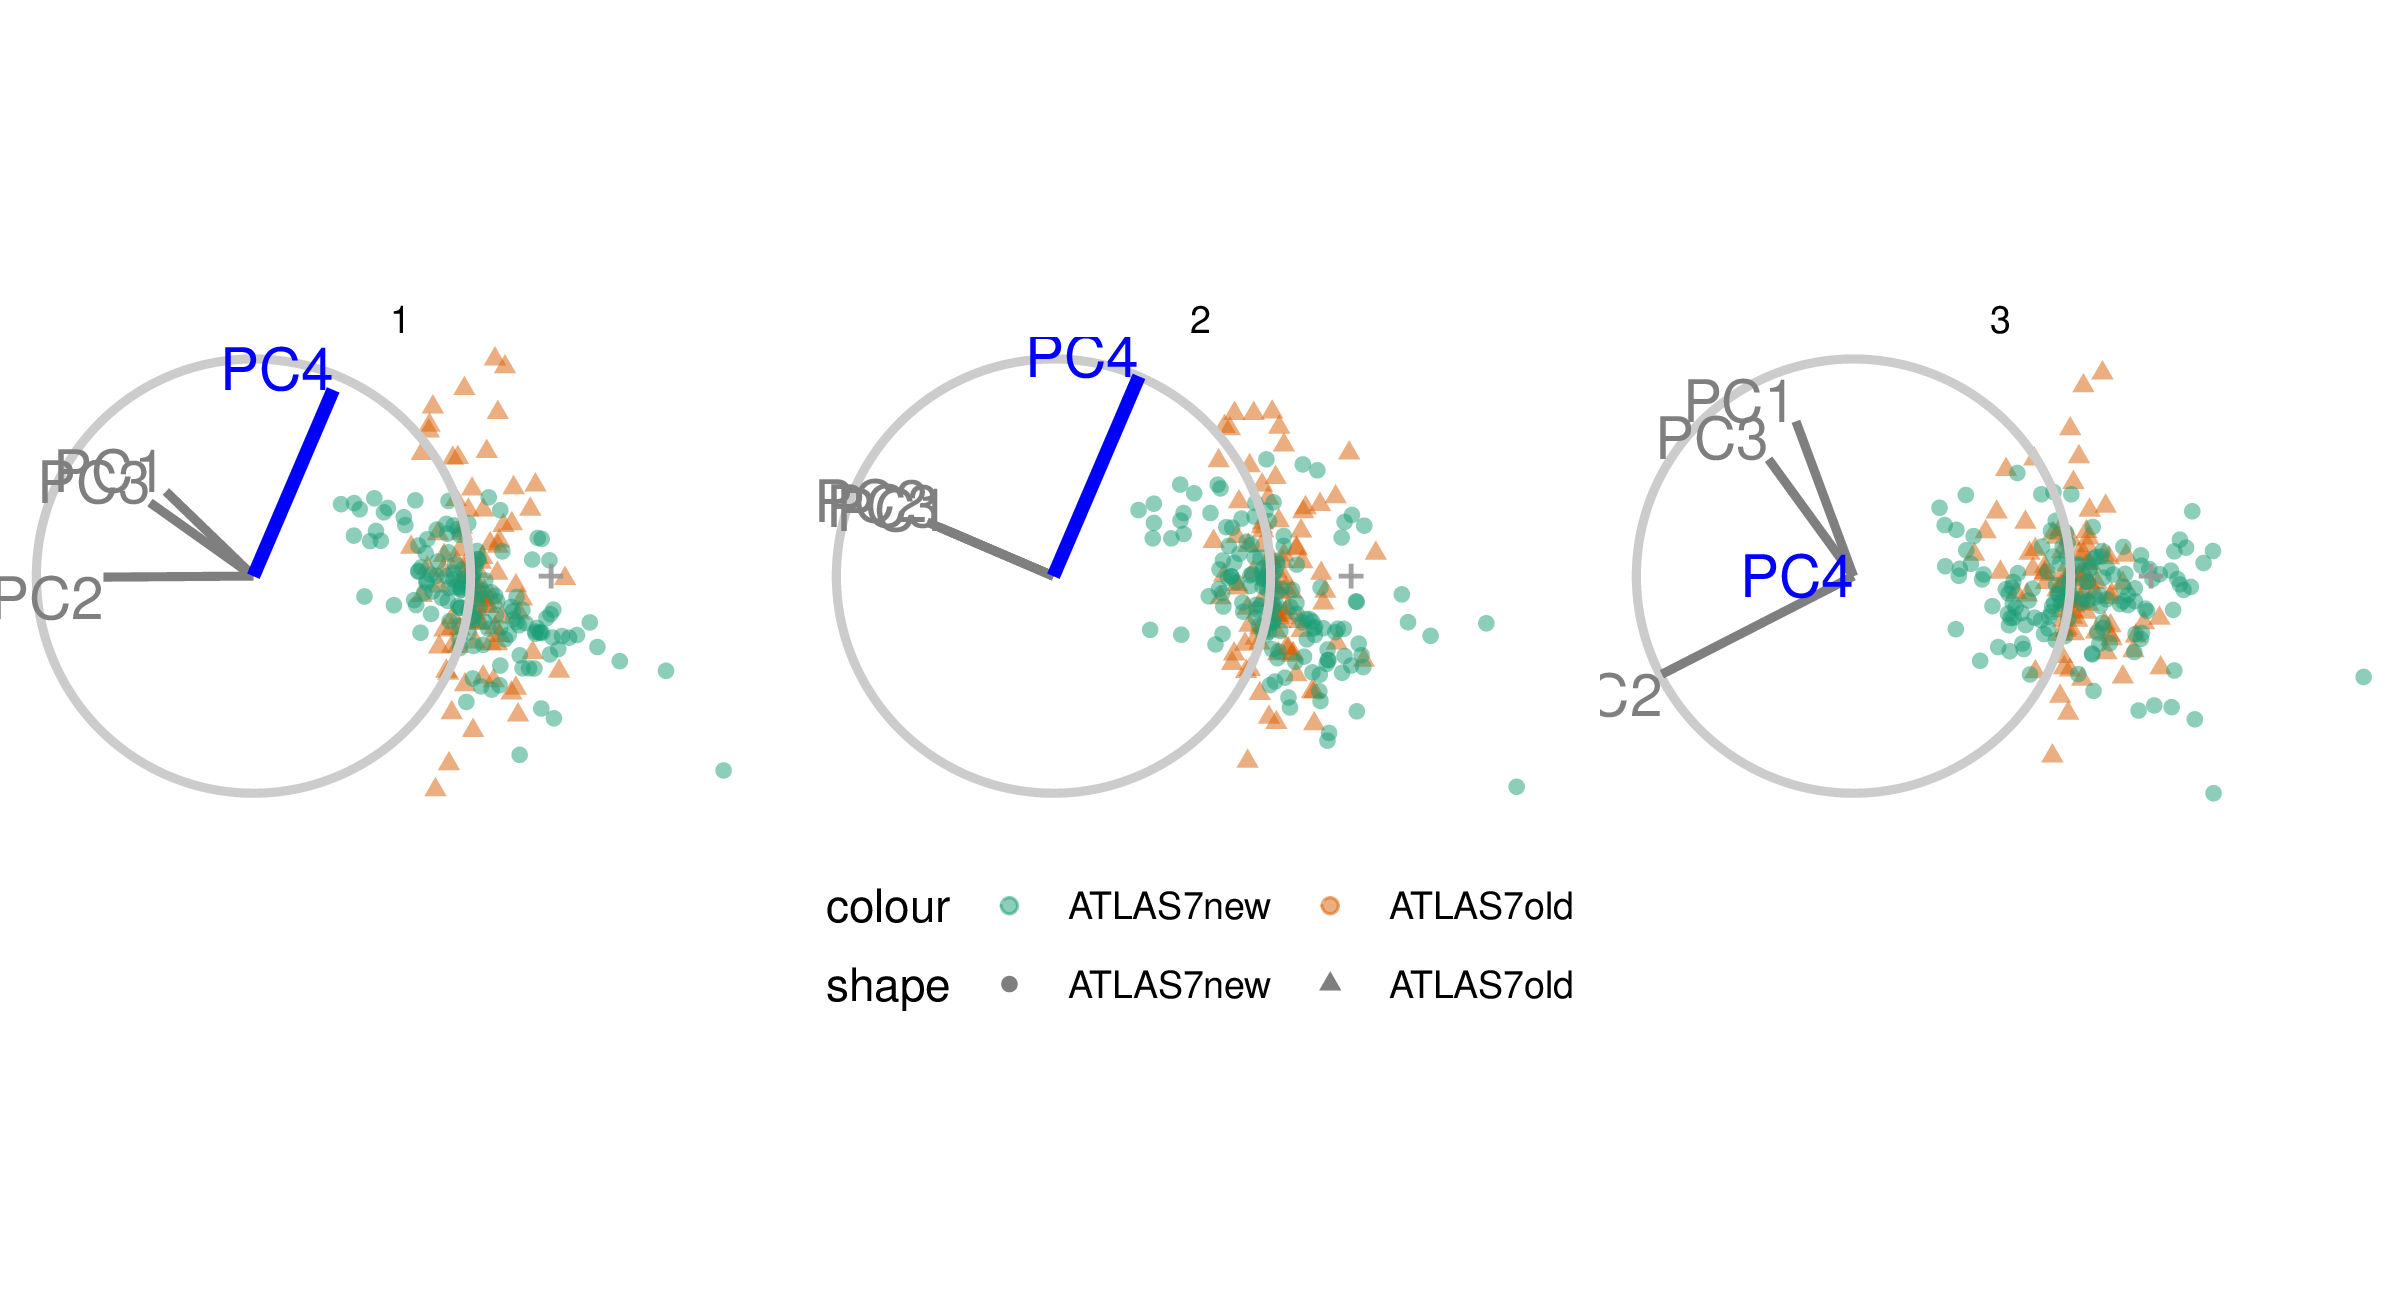
\includegraphics[width=1\linewidth,]{./figures_from_script/ch3_fig4_jet_better_pc4} 

}

\caption{Select frames from a radial tour of PC4 within the jet cluster, with color indicating experiment type: ATLAS7new (green) and ATLAS7old (orange). When PC4 is removed from the projection (frame 10) there is little difference between the clusters, suggesting that PC4 is important for distinguishing the experiments.}\label{fig:ch3fig4}
\end{figure}

\begin{figure}

{\centering 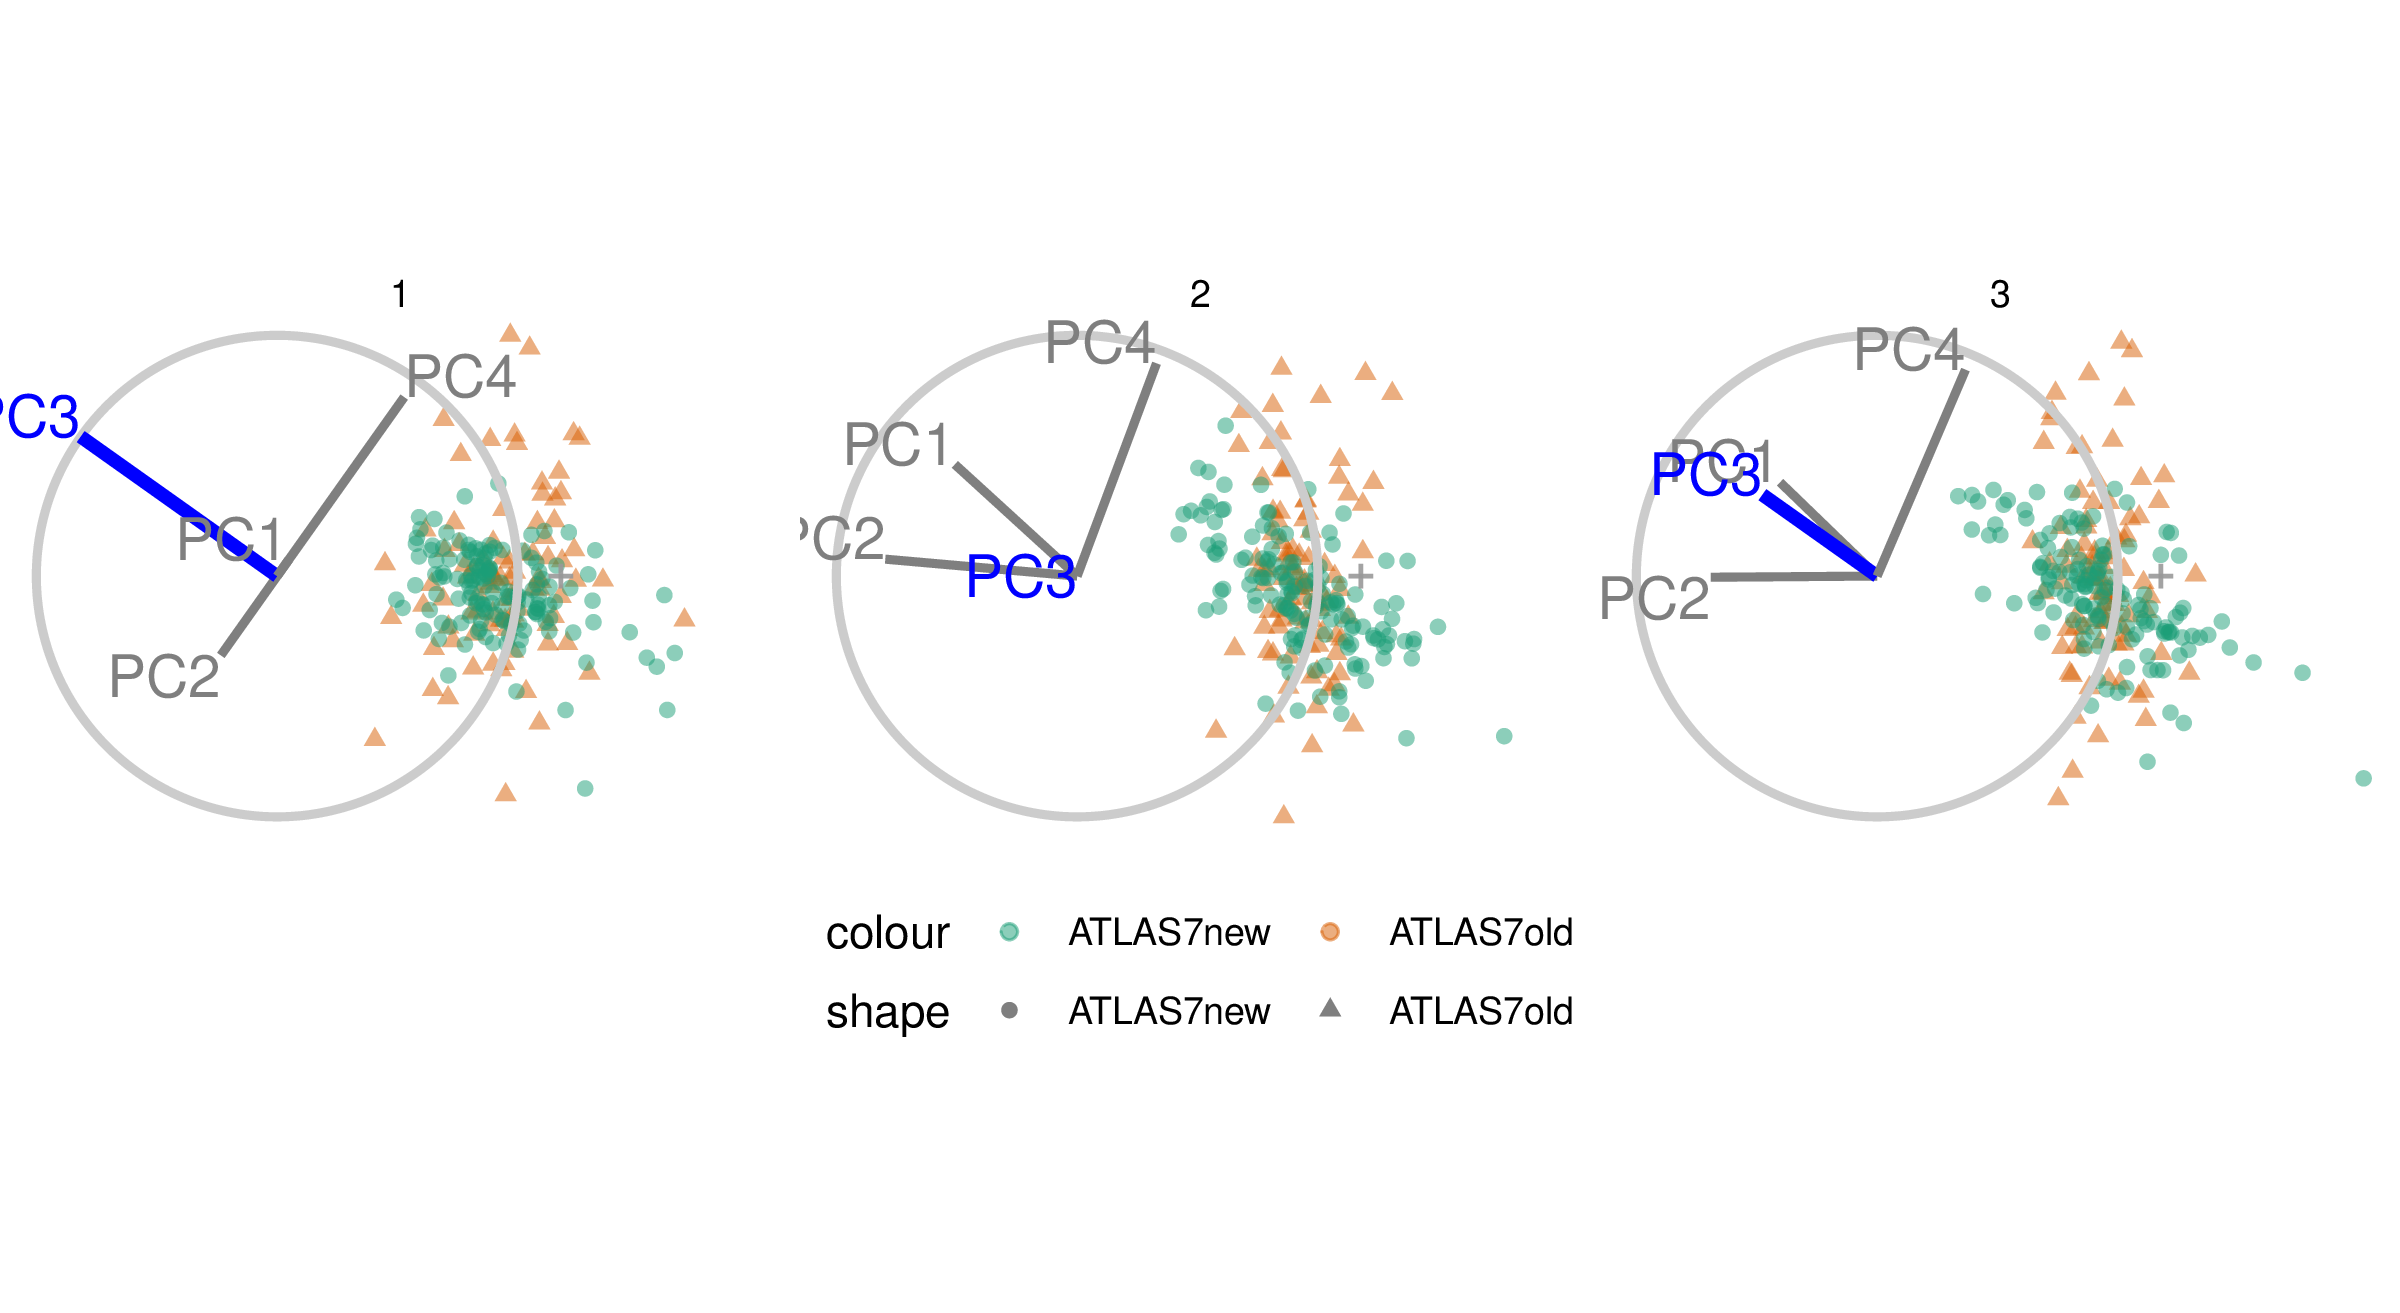
\includegraphics[width=1\linewidth,]{./figures_from_script/ch3_fig5_jet_worse_pc3} 

}

\caption{Frames from the radial tour manipulating PC3 within the jet cluster, with color indicating experiment type: ATLAS7new (green) and ATLAS7old (orange).  When the contribution from PC3 is changed there is little change in the separation of the clusters, suggesting that PC3 is not important for distinguishing the experiments.}\label{fig:ch3fig5}
\end{figure}

\hypertarget{dis-cluster}{%
\subsection{DIS cluster}\label{dis-cluster}}

Following \textcite{cook_dynamical_2018}, to explore the DIS cluster, PCA is recomputed and the first six principal components, explaining 48\% of the full sample variation, are used. The contributions of PC6 and PC2 are explored in Figures \ref{fig:ch3fig6} and \ref{fig:ch3fig7}, respectively. Three experiments are examined: DIS HERA1+2 (green), dimuon SIDIS (purple), and charm SIDIS (orange).

Both PC2 and PC6 contribute to the projection similarly. When PC6 is rotated into the projection, variation in the DIS HERA1+2 is greatly reduced. When PC2 is removed from the projection, dimuon SIDIS becomes more clearly distinct. Even though both variables contribute similarly to the original projection, their contributions have quite different effects on the structure of each cluster, and the distinction between clusters. Animations of all of the principal components can be viewed from the links: \href{https://github.com/nspyrison/spinifex_paper/blob/master/paper/gifs/discluster_manualtour_pc1.gif}{PC1}, \href{https://github.com/nspyrison/spinifex_paper/blob/master/paper/gifs/discluster_manualtour_pc2.gif}{PC2}, \href{https://github.com/nspyrison/spinifex_paper/blob/master/paper/gifs/discluster_manualtour_pc3.gif}{PC3}, \href{https://github.com/nspyrison/spinifex_paper/blob/master/paper/gifs/discluster_manualtour_pc4.gif}{PC4}, \href{https://github.com/nspyrison/spinifex_paper/blob/master/paper/gifs/discluster_manualtour_pc5.gif}{PC5}, and \href{https://github.com/nspyrison/spinifex_paper/blob/master/paper/gifs/discluster_manualtour_pc6.gif}{PC6}.

\begin{figure}

{\centering 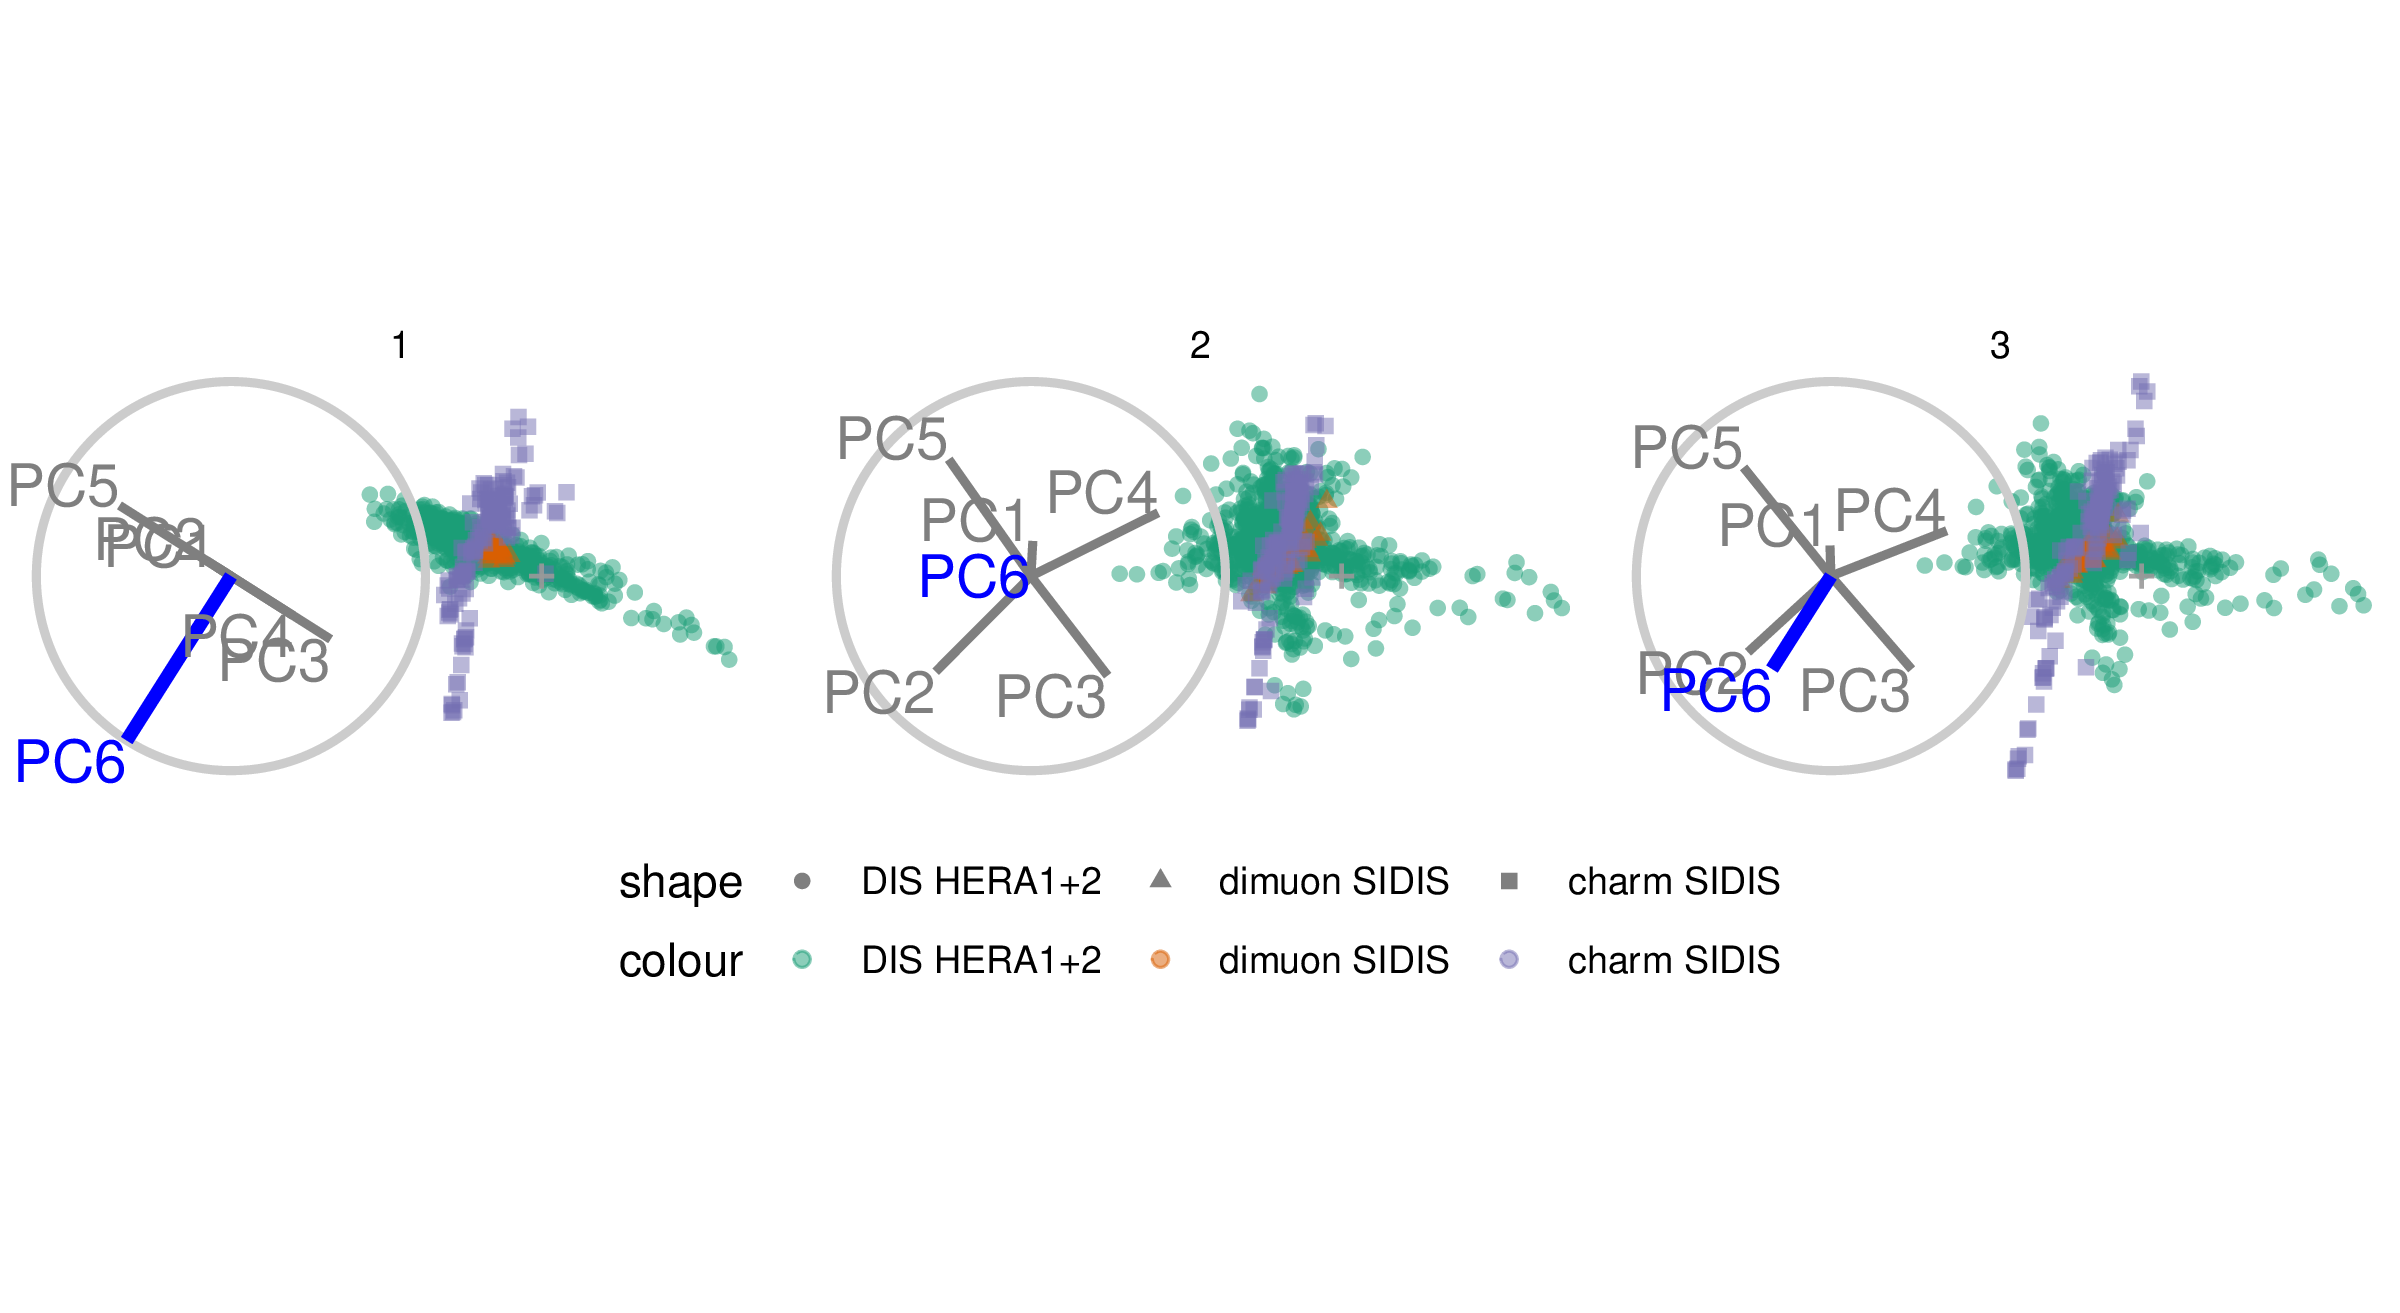
\includegraphics[width=1\linewidth,]{./figures_from_script/ch3_fig6_DIS_better_pc6} 

}

\caption{Select frames from a radial tour exploring the sensitivity that PC6 has on the structure of the DIS cluster, with color indicating experiment type: DIS HERA1+2 (green), dimuon SIDIS (purple), and charm SIDIS (orange). DIS HERA1+2 is distributed in a cross-shaped plane, charm SIDIS occupies the center of this cross, and dimuon SIDIS is a linear cluster crossing DIS HERA1+2. As the contribution of PC6 is increased, DIS HERA1+2 becomes almost singular in one direction (frame 5), indicating that this cluster has very little variability in the direction of PC6.}\label{fig:ch3fig6}
\end{figure}

\begin{figure}

{\centering 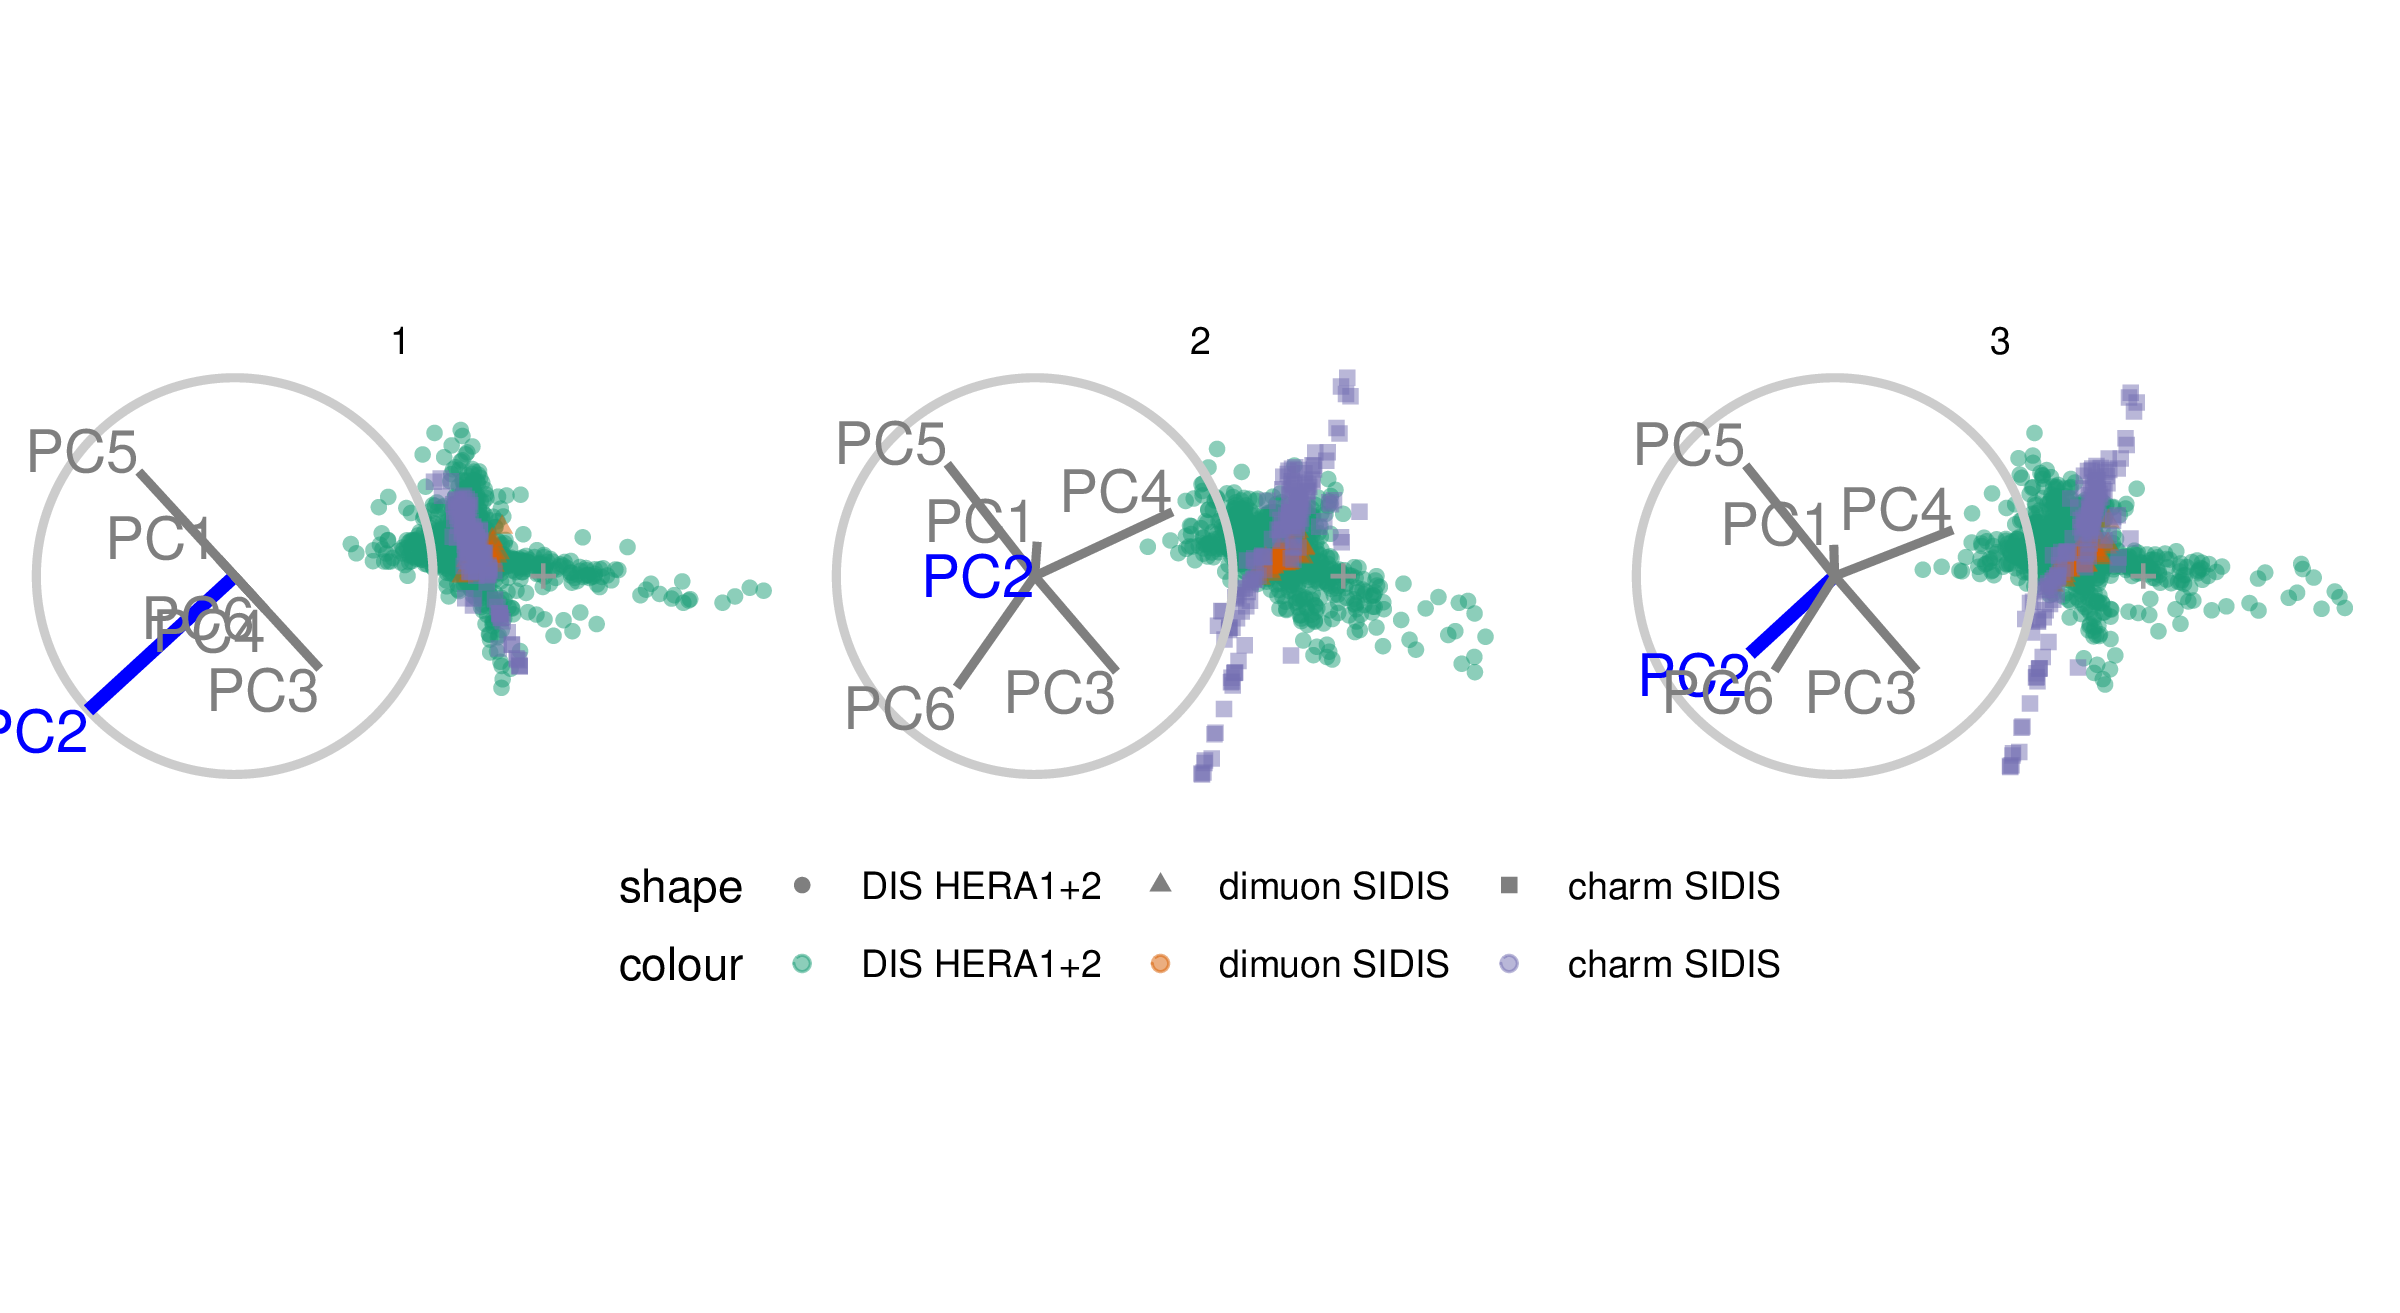
\includegraphics[width=1\linewidth,]{./figures_from_script/ch3_fig7_DIS_worse_pc2} 

}

\caption{Frames from the radial tour exploring the sensitivity PC2 to the structure of the DIS cluster, with color indicating experiment type: DIS HERA1+2 (green), dimuon SIDIS (purple), and charm SIDIS (orange). As contribution from PC2 is decreased, dimuon SIDIS becomes more distinguishable from the other two clusters, indicating that in its absence PC2 is important for separating this cluster from the others.}\label{fig:ch3fig7}
\end{figure}

\hypertarget{sec:discussion}{%
\section{Discussion}\label{sec:discussion}}

Dynamic linear projections of numeric multivariate data, tours, play an important role in data visualization; they extend the dimensionality of visuals to peek into high-dimensional data and parameter spaces. This research has taken the manual tour algorithm, specifically the radial rotation, used in GGobi \autocite{swayne_ggobi:_2003} to interactively rotate a variable into or out of a 2D projection, and modified it to create an animation that performs the same task. It is most useful for examining the importance of variables, and how the structure in the projection is sensitive or not to specific variables. This functionality available in package \{spinifex\}. The work complements the methods available in the \{tourr\} package.

This work was motivated by problems in physics, and thus the usage was illustrated on data comparing experiments of hadronic collisions, to explore the sensitivity of cluster structure to different principal components. These tools can be applied quite broadly to many multivariate data analysis problems.

The manual tour is constrained in the sense that the effect of one variable is dependent on the contributions of other variables in the manip space. However, this can be useful to simplify a projection by removing variables without affecting the visible structure. Defining a manual rotation in high dimensions is possible using Givens rotations and Householder reflections as outlined in \textcite{buja_computational_2005}. This would provide more flexible manual rotation, but more difficult for a user because they have the choice (too much choice) of which directions to move.

Another future research topic could be to extend the algorithm for use on 3D projections. With the current popularity and availability of 3D virtual displays, this may benefit the detection and understanding of the higher dimensional structure, or enable the examination of functions.

Having a graphical user interface would be useful for making it easier and more accessible to a general audience. This is possible to implement using \{shiny\} \autocite{chang_shiny_2020}. The primary purposes of the interface would be to allow the user to interactively change the manip variable easily, and the interpolation step for more or less detailed views.

\hypertarget{acknowledgments-1}{%
\section{Acknowledgments}\label{acknowledgments-1}}

This article was created in R, using \{knitr\} \autocite{xie_knitr_2020} and \{rmarkdown\} \autocite{allaire_rmarkdown_2020}, with code generating the examples inline. The source files for this article be found at \href{https://github.com/nspyrison/spinifex_paper/}{github.com/nspyrison/spinifex\_paper/}. The animated gifs can also be viewed at this site, and also in the supplementary material for this paper. The source code for the \{spinifex\} package can be found at \href{https://github.com/nspyrison/spinifex/}{github.com/nspyrison/spinifex/}.

\hypertarget{ch:efficacy_radial_tour}{%
\chapter{The benefit of user-controlled radial tour for understanding variable contributions to structure in linear projections}\label{ch:efficacy_radial_tour}}

THIS CHAPTER IS CURRENTLY BEING EDITED IN IT's OWN REPOSITORY, THIS VERSION IS OUT OF DATE.

TODO:XXX Segue. Bring over abstract?

\hypertarget{introduction-1}{%
\section{Introduction}\label{introduction-1}}

Multivariate data underlies most classification problems. Yet exploratory data analysis \autocite[EDA,][]{tukey_exploratory_1977} of such spaces is difficult, increasingly so as dimension increases, and often leads to the consideration of models for these problems being considered to be black-boxes. There is increasing emphasis on the need to provide explainers to improve the interpretability for black-box models \autocite{biecek_dalex_2018,biecek_explanatory_2021,lundberg_unified_2017,ribeiro_why_2016,wickham_visualizing_2015}. Visualization is an important part of providing interpretations \autocite{anscombe_graphs_1973,coleman_geometric_1986,goodman_dirty_2008,matejka_same_2017}. Tour methods \autocite{lee_review_2021,cook_grand_2008} provide ways to visualize linear projections of high-dimensional spaces, to obtain an overview of shape (distributions and associations) and anomalies (outliers, clusters). The recently introduced radial tour \autocite{spyrison_spinifex_2020} provides a user-controlled manual rotation of variables into and out of a projection, which might especially be useful for studying variable importance.

Dimension reduction is commonly used in conjunction with visualization to provide informative low-dimensional summaries of high-dimensional data. There have been several user studies
for dimension reduction comparing across embeddings and display dimensionality \autocite{gracia_new_2016,wagner_filho_immersive_2018}. There are also empirical metrics and comparisons used to describe non-linear reduction and how well and faithfully they embed the data \autocite{bertini_quality_2011,liu_visualizing_2017,sedlmair_empirical_2013,van_der_maaten_visualizing_2008}. There is an absence of studies comparing techniques for assessing variable importance, particularly, how best to convey information to the viewer.

This paper describes a user study conducted to assess the benefit of the radial tour, in comparison with principal component analysis and a grand tour for understanding variable importance. The experiment is a within-participant user study. The type of visualization is the primary factor of the study, corresponding to a null hypothesis that all techniques provide a similar ability for the user to determine variable importance. The techniques are compared by having subjects complete several tasks, where accuracy and speed are recorded.

The paper is structured as follows. Section \ref{sec:background} provides the background on the visualization methods being compared. Section \ref{sec:userstudy} describes the user study, the tasks, evaluation, and measures used. The results of the study are in Section \ref{sec:results}. Conclusions and potential future directions are discussed in Section \ref{sec:conclusion}. The software used for the study is described in Section \ref{sec:spinifex}.

\hypertarget{sec:background}{%
\section{Background}\label{sec:background}}

\hypertarget{principal-component-analysis}{%
\subsection{Principal component analysis}\label{principal-component-analysis}}

Principal component analysis is a good baseline of comparison for linear projections because of its frequent and broad use across disciplines. Principal component analysis \autocite[PCA,][]{pearson_liii._1901} creates new components that are linear combinations of the original variables. The creation of these variables is ordered by decreasing variation which is orthogonally constrained to all previous components. While the full dimensionality is intact, the benefit comes from the ordered nature of the components. The first 2 or 3 components are typically used to approximate the variation multivariate data set, while the rest are discarded.

\begin{figure}

{\centering 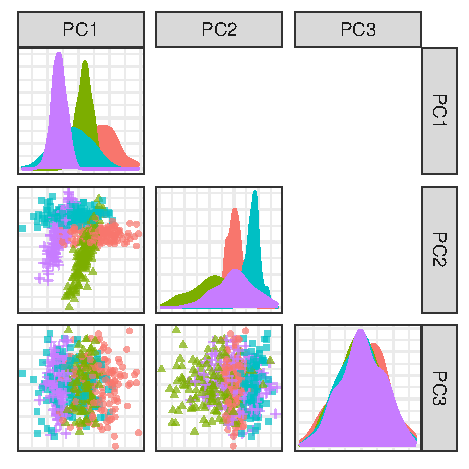
\includegraphics[width=1\linewidth,]{./figures_from_script/ch4_fig1_pca_splom} 

}

\caption{Scatterplot matrix of the first 3 principal components for simulated data. Traditional multivariate visualization of *data*-space involes static display of the first several principal components.}\label{fig:ch4fig1}
\end{figure}

\hypertarget{scatterplot-matrix}{%
\subsection{Scatterplot matrix}\label{scatterplot-matrix}}

An extension to showing only a few components is to show pairs of components as a scatterplot matrix \autocite{chambers_graphical_1983}, where all pairs of the components are displayed on the upper or lower triangles of the matrix. This is a convenient way to fit many plots onto a page, but when there are many variables there is insufficient space on a page to display them all. Figure \ref{fig:ch4fig1} shows the first three components of simulated data as a scatterplot matrix.

\hypertarget{data-visualization-tours}{%
\subsection{Data visualization tours}\label{data-visualization-tours}}

A data visualization \emph{tour} uses time to animate local changes in the projection basis. One of the key features of the tour is the object permanence of the data points; that is to say by watching nearby frames one can track the relative changes of observations as the basis moves toward the next target basis. There are various types of tours that are distinguished by the selection or generation of their basis paths \autocite{lee_review_2021,cook_grand_2008}. To contrast with the discrete orientations of PCA, we compare with continuous changes of linear projection with \emph{grand} and \emph{radial} tours.

\hypertarget{grand-tours}{%
\subsubsection{Grand tours}\label{grand-tours}}

In a grand tour \autocite{asimov_grand_1985} the target bases are selected randomly. The grand tour is the first and most widely known tour. It will serve as an intermediate unit of comparison which has continuity of data points in nearby frames along with the radial tour but lacks the user control enjoyed by PCA and radial tours. This lack of control makes grand tours more of a generalist exploratory tool.

\hypertarget{radial-manual-tours}{%
\subsubsection{Radial (manual) tours}\label{radial-manual-tours}}

The \emph{manual} tour \autocite{cook_manual_1997} defines its basis path by manipulating the basis contribution of a selected variable. A manipulation dimension is appended onto the projection plane, with a full contribution given to the selected variable. The target bases are then selected based on rotating this newly created manipulation space. The target bases are then similarly orthogonally restrained, data projected, and rendered into an animation. For the variables to remain independent of each other, the contributions of the other variables must also change, \emph{ie.} dimension space should maintain its orthonormal structure. A key feature of the manual tour is that it affords users a way to control the variable contributions of the next target basis. This means that such manipulations can be selected and queued in advance or select on the spot for human-in-the-loop analysis \autocite{karwowski_international_2006}. However, this navigation is relatively time-consuming due to the huge volume of \(p\)-space (an aspect of the curse of dimensionality \autocite{bellman_dynamic_1957}) and the abstract method of steering the projection basis. It is advisable to first identify a basis of particular interest and then use a manual tour as a finer, local exploration tool to observe how the contributions of the selected variable do or do not contribute to the feature of interest.

To simplify the task and keep its duration realistic, we consider a variant of the manual tour, called a \emph{radial} tour. In a radial tour, the selected variable is allowed to change its magnitude of contribution, but not its angle; it must move along the direction of its original contribution radius. The radial tour benefits from both continuity of the data alongside grand tours, but also allows the user to steer via choosing the variable to rotate.

The recent implementation of manual tours us the R package \{spinifex\} \autocite{spyrison_spinifex_2020}, which facilitates manual tours (and radial variant). It is also compatible with tours made with \{tourr\} \autocite{wickham_tourr:_2011} and facilitates exporting to .gif or .html widget, with recent graphic packages. Now that we have a readily available means to produce various tours, we want to see how they fare against traditional discrete displays commonly used with PCA.

\hypertarget{sec:userstudy}{%
\section{User study}\label{sec:userstudy}}

An experiment was constructed to assess the performance of the radial tour relative to the tour and scatterplots of principal components for interpreting the importance of variables to class separations.

The three methods were examined for three different cluster shapes, using different combinations of contributing variables, and data dimensionality. Data was collected using a specially constructed web app, through crowd-sourced with prolific.co \autocite{palan_prolific_2018}.

\hypertarget{sec:blocks}{%
\subsection{Experimental factors}\label{sec:blocks}}

In addition to visual factor, we vary the data across 3 aspects: 1) The \emph{location} of the difference between clusters, by mixing a signal and a noise variable at different ratios, we vary the number of variables and their magnitude of cluster separation, 2) the \emph{shape} of the clusters, to reflect different distributions of the data, and 3) the \emph{dimension}-ality of the data.

\begin{figure}

{\centering 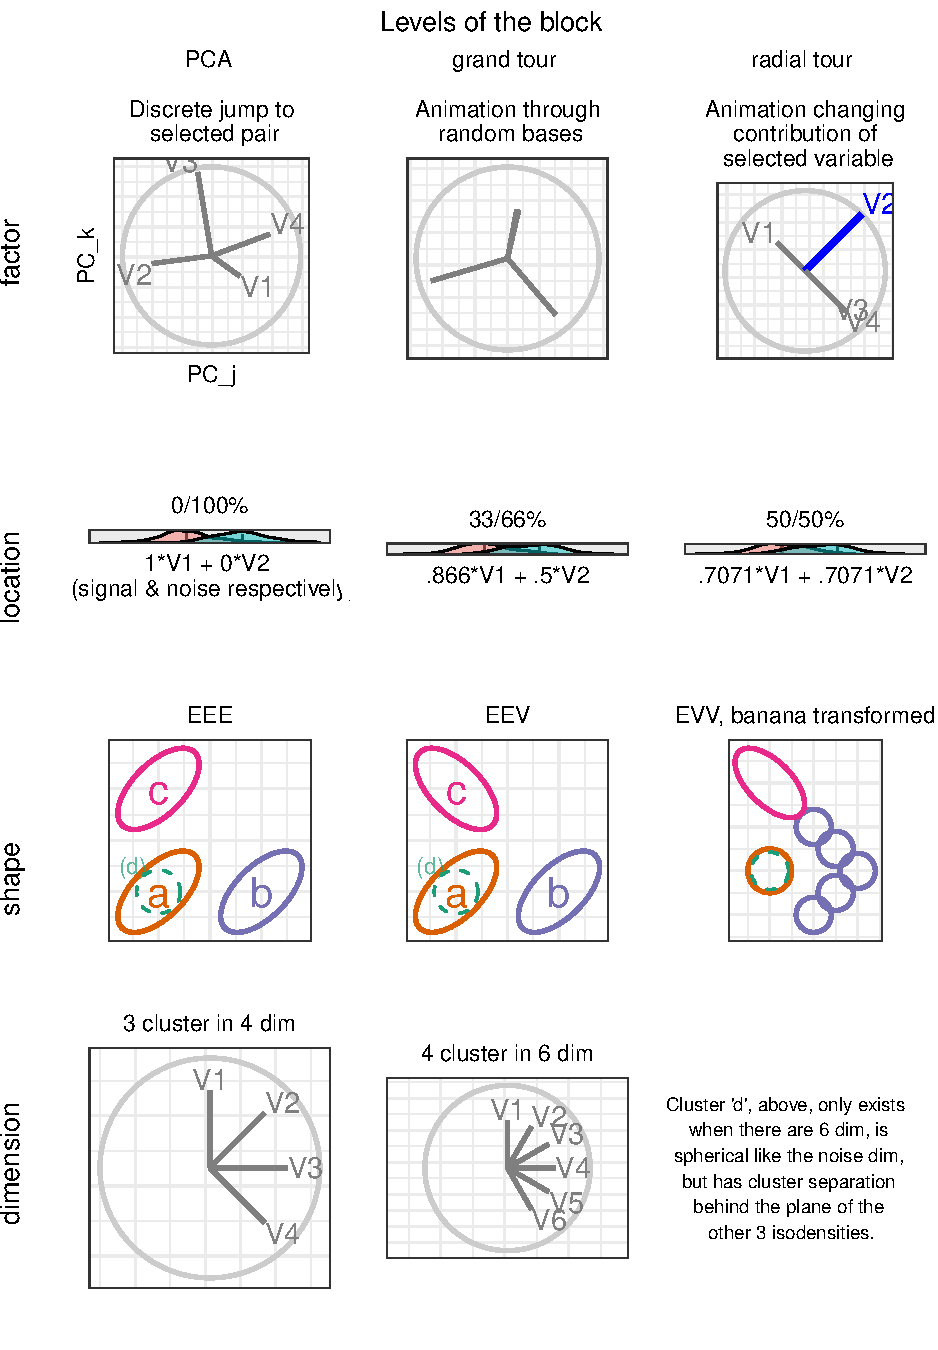
\includegraphics[width=1\linewidth,]{./figures_from_script/ch4_fig2_exp_factors} 

}

\caption{Illustration of the experimental factors: visualization factor, the variable location of the cluster separationm, the shape of the clusters, and the dimensionality (and clusters) of the data.}\label{fig:ch4fig2}
\end{figure}

The \emph{location} of the separation of the clusters is a crucial aspect of analysis, it is the variables or combination their of that is important to the explanation of the structure. To test the sensitivity to this we mix a noise-variable with the signal-containing variable such that the difference in the clusters is mixed at the following percentages: 0/100\% (not mixed), 33/66\%, 50/50\% (evenly mixed).

In selecting the \emph{shape} of the clusters we follow the convention given by \textcite{scrucca_mclust_2016}, where 14 variants of model families containing 3 clusters are defined. The name of the model family is the abbreviation of its respective volume, shape, and orientation of the cluster, which are either equal or vary. We use the models EEE, EEV, and EVV, the latter is further modified by moving 4 fifths of the data out in a ``V'' or banana-like shape. Figure \ref{fig:ch4fig2} shows the principal component isodensity of the 3 model variants applied here.

\emph{Dimension}-ality is tested at 2 modest levels, namely, in 4 dimensions containing 3 clusters and 6 dimensions with 4 clusters. We must do so to bound the difficulty and search space to keep the task realistic for crowdsourcing.

\hypertarget{sec:objective}{%
\subsection{Objective}\label{sec:objective}}

PCA will be used as a baseline for comparison as it is the most common linear embedding. The grand tour will act as a secondary control that will help evaluate the benefit of animation, with the persistence of the data points across changes in basis, but without the ability to influence its path. Lastly, the radial tour should perform best as it benefits both from animation and being able to select an individual variable to change the contribution. Next we cover how we expect them to perform and state the hypothesis to test.

Then for some subset of tasks, we expect to find that the radial tour performs most accurately, as it enjoys both the persistence of points and input control to explore specific variables. Secondly, it may be the case that grand performs faster than the alternatives with its absence of inputs, users can focus all of their attention on interpreting the fixed path. Conversely, we are less certain about the accuracy of such a limited grand tours as there is no objective function in the target bases; it is possible that, by chance, the planes completely avoid the information needed. However, given that the data dimensionality will be modest, it seems likely that grand tour regularly crosses frames with the correct information to perform the task quickly.

We measure the accuracy and speed over the support of the discussed experimental factors. The null hypotheses can be stated as:

\(~~~~~H_0: \text{visualization factor does not impact task } \textit{accuracy}, Y_1. \\\)
\(~~~~~~H_0: \text{visualization factor does not impact task } \textit{speed}, Y_2. \\\)

\hypertarget{sec:task}{%
\subsection{Task and evaluation}\label{sec:task}}

With our hypothesis formulated let's turn our attention to the task and how to evaluate it.
Recall that the display was a 2D scatterplot with axis biplot to its left. Observations were supervised with the cluster level coded by color and shape.

Participants were asked to `check any/all variables that contribute more than average to the cluster separation green circles and orange triangles', which was further explained in the explanatory video as `mark and all variable that carries more than their fair share of the weight, or 1 quarter in the case of 4 variables'.

The instructions iterated several times in the video was: 1) Use the input controls to find a frame that contains separation between the clusters of green circles and orange triangles, 2) look at the orientation of the variable contributions in the gray circle, a visual depiction of basis, and 3) select all variables that contribute more than average in the direction of the separation in the scatterplot. Regardless of factor and block values participants were limited to 60 seconds for each evaluation of this task.

The evaluation measure of this task was designed with a couple of features in mind: 1) the sum of squares of the individual variable marks should be 1, and 2) symmetric about 0, without preference to under- or over-guessing. With these in mind, we define the following measure for evaluating the task.

Let a dataset \(\textbf{X}\) be a simulation containing clusters of observations of different distributions. Let \(\textbf{X}_k\) be the subset of observations in cluster \(k\) containing the \(p\) variables.

\begin{align*}
W_{j} &=\frac
{(\overline{X_{j=1, k=1}} - \overline{X_{1, k=2}}, ~...~
(\overline{X_{j=p, k=1}} - \overline{X_{j=p, k=2}})}
{\sum_{j=1}^{p}(|\overline{X_{j,k=1}} - \overline{X_{j,k=2}}|)}
- \frac{1}{p} \\
\\
\text{Accuracy}, Y &= \sum_{j=1}^{p}I(r_j) * sign(w_j) * \sqrt{|w_j|}  \\
\end{align*}

where \(I\) is the indicator function. Then the total marks for this task is the sum of this marks vector. We use the time till the last response as a secondary dependent variable \(Y_2\).

\begin{figure}

{\centering 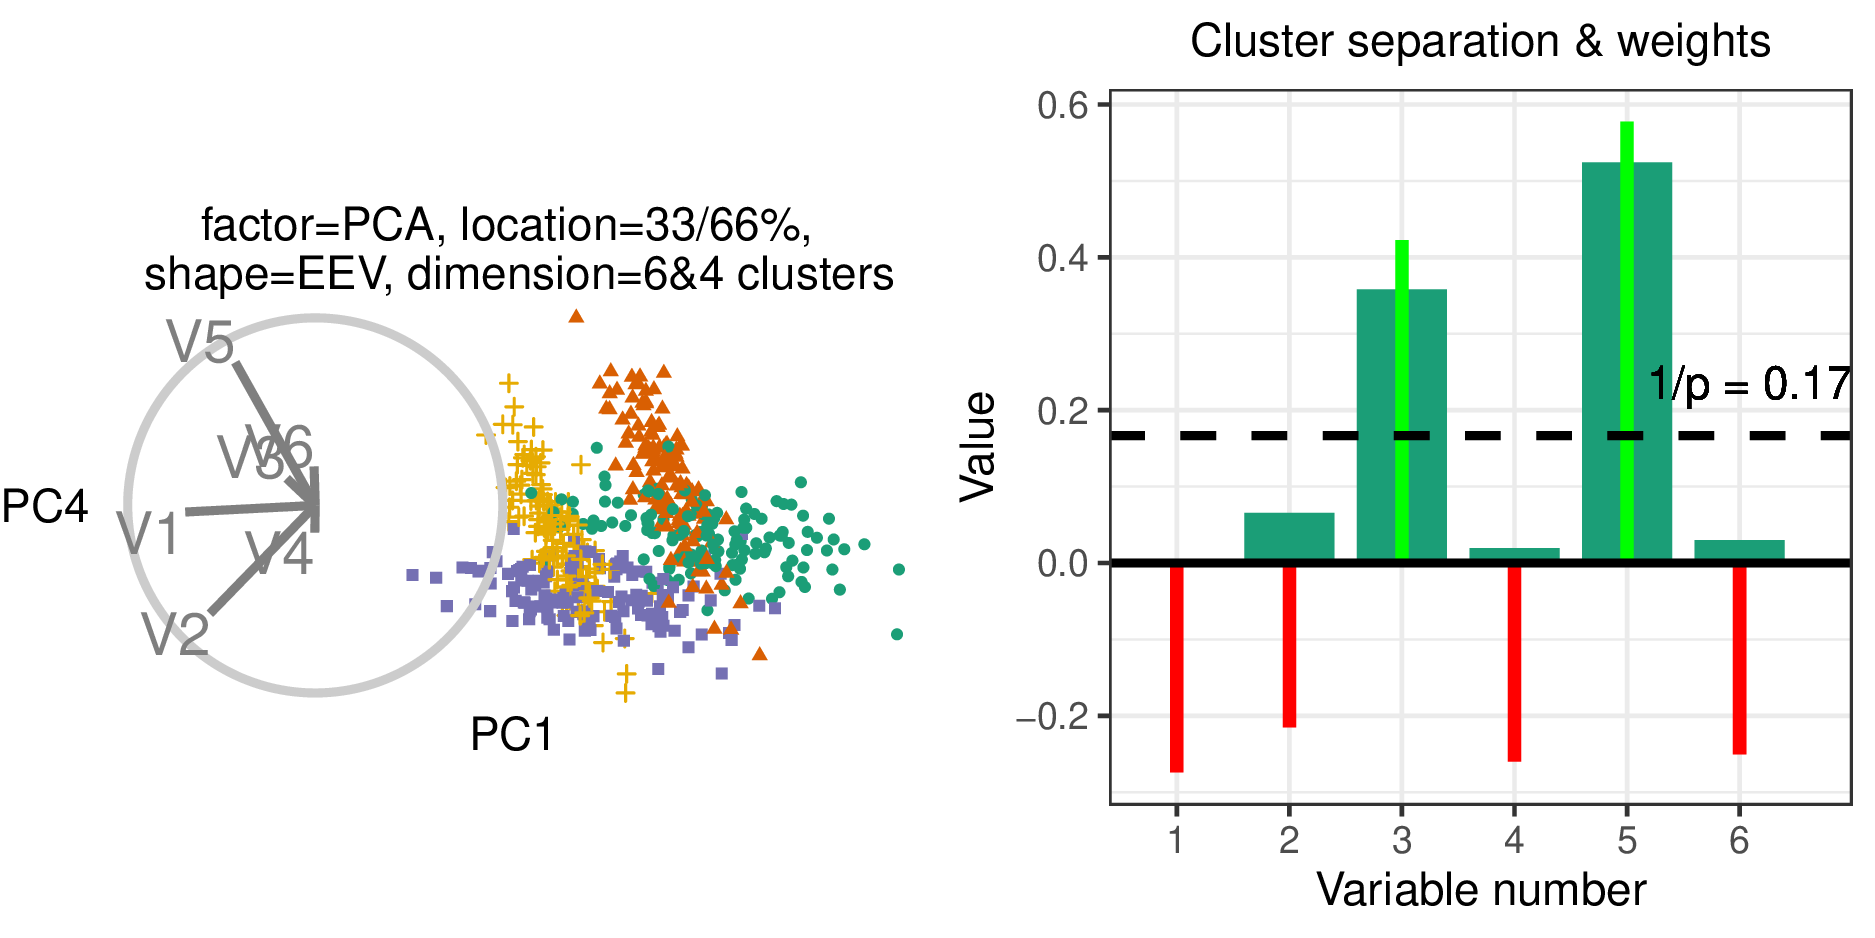
\includegraphics[width=1\linewidth,]{./figures_from_script/ch4_fig3_accuracy_measure} 

}

\caption{(L), PCA biplot of the components showing the most cluster separation with (R) illustration of the magnitude of cluster separation is for each variable (wide bar) and the weight of the marks given if a variable is selected (red/green line). The horizontal dashed line is 1 / dimensionality, the amount of separation each variable would have if evenly distributed. The weights equal the signed square of the difference between each variable value and the dashed line.}\label{fig:ch4fig3}
\end{figure}

\hypertarget{sec:standardization}{%
\subsection{Visual design standardization}\label{sec:standardization}}

Section \ref{sec:background} gives the sources and a description of the visual factors PCA, grand tours, and radial manual tours. The factors are tested within-participant, with each factor being evaluated by each participant. The order that factors are experienced is controlled with the block assignment as illustrated below in Figure \ref{fig:ch4fig4}. Below we cover the visual design standardization, as well the input and display within each factor.

The visualization methods were standardized wherever possible. each factor was shown as a biplot, with variable contributions displayed on a unit circle. All aesthetic values (colors, shapes, sizes, absence of legend, and absence of axis titles) were held constant. Variable contributions were always shown left of the scatterplot embeddings with their aesthetic values consistent as well. What did vary between factors were their inputs which caused a discrete jump to another pair or principal components, were absent for the grand tour with target bases to animate through selected at random, or for the radial tour which variable should have its contribution animated.

PCA inputs allowed for users to select between the top 4 principal components for both the x and y-axis regardless of the data dimensionality (either 4 or 6). There was no user input for the grand tour, users were instead shown a 15-second animation of the same randomly selected path. Users were able to view the same clip up to 4 times within the time limit. Radial tours were also displayed at 5 frames per second within the interpolation step size of 0.1 radians. Users were able to swap between variables, upon which the display would change the start of radially increasing the contribution of the selected variable till it was full, zeroed, and then back to its initial contribution. The complete animation of any variable takes about 20 seconds and is almost fully in the projection frame at around 6 seconds. The starting basis of each is initialized to a half-clock design, where the variables were evenly distributed in half of the circle which is then orthonormalized. This design was created to be variable agnostic while maximizing the independence of the variables.

\hypertarget{data-simulation-task}{%
\subsection{Data simulation, task}\label{data-simulation-task}}

Each dimension is originally distributed as \(\mathcal{N}(2 * I(signal), 1)~|~\text{covariance}~\Sigma\), a function of the shape. Signal variables have a correlation of 0.9 when they have equal orientation and -0.9 when their orientations vary. Noise variables were restricted to 0 correlation. Each cluster is simulated with 140 observations and is offset in a variable that does not separate previous variables.

Clusters of the EVV shape are transformed to the banana-chevron shape. Then location mixing is applied by post-multiplying a (2x2) rotation matrix to the signal variable and a noise variable for the clusters in question.

All variables are then standardized by standard deviation. The rows and columns are then shuffled randomly. The observation's cluster and order of shuffling are attached to the data and saved.

Each of these replications are then iterated with each level of the factor. For PCA, every pair of the top 4 principal components and saved as 12 plots. For the grand tour, we first save 2 basis paths (for 4 and 6 dimension), each replication is then projected through the common basis path as the variable(s) containing the were previously shuffled. The resulting animations were saved as .gif files. The radial tour starts at either the 4 or 6-variable ``half-clock'' basis, where each variable has a uniform contribution, and no variable contributing in the opposite direction (to minimize variable dependence), a radial tour is then produced for each variable and saved as a .gif.

\hypertarget{data-collection-and-factor-assignment}{%
\subsection{Data collection, and factor assignment}\label{data-collection-and-factor-assignment}}

Now, with simulation and their artifacts in hand. We explain how the experimental factors are assignment, and illustrate how this is experienced from a participant's perspective.

We section the study into 3 periods, each period is linked to a randomized level of both the factor visualization and the location. The order of dimension and shape are of secondary interest and are held constant in increasing order of difficultly; 4 then 6 dimensions and EEE, EEV, then EVV-banana respectively.

The period starts with an untimed training task at the simplest remaining block parameterization; location = 0/100\%, shape = EEE, and 4 dimensions with 3 clusters. This serves to introduce and familiarize participants with input and visual differences. After the training, the participant is evaluated on 2 tasks with the same factor * location level, across the increasing difficulty of dimension * shape. These evaluations removed the plot after 60 seconds, though this limit was rarely reached by participants.

The order of the levels of the factor and location is randomized with a nested Latin square where all levels of factor are exhausted before advancing to the next level of location. That means we need \(3!^2 = 36\) participants to perform a full block evaluation. This randomization is important to control for any potential learning effects the participant may receive. Figure \ref{fig:ch4fig4} illustrates how an arbitrary participant experiences the experimental factors.

\begin{figure}

{\centering 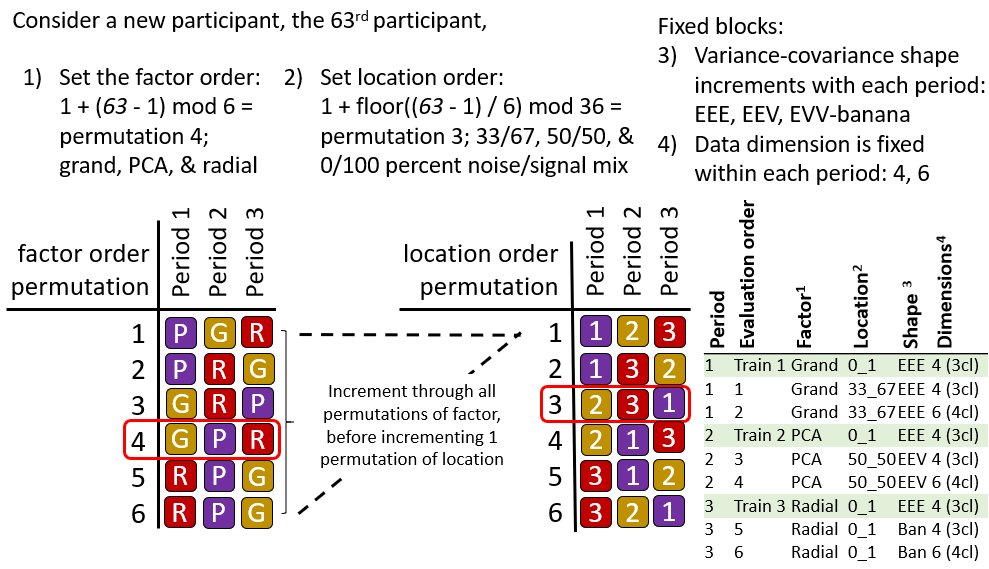
\includegraphics[width=1\linewidth,]{./figures_from_script/ch4_fig4_randomization_MANUAL} 

}

\caption{Illustration of the nested latin square and how a hypothetical participant 63 is assigned factor and block parameterizations. Each of the 6-factor permutations is exhausted before iterating to the next permutation of location.}\label{fig:ch4fig4}
\end{figure}

Through pilot studies sampled by convenience (information technology and statistics Ph.D.~students attending Monash University), we predict that we need 3 full evaluations to properly power our study; we set out to crowdsource \(N = 3 * 3!^2 = 108\) participants.

\hypertarget{sec:subjects}{%
\subsection{Recruiting subjects}\label{sec:subjects}}

We recruited \(N = 108\) participants via prolific.co \autocite{palan_prolific_2018}. We filtered participants based on their claimed education requiring that they have completed at least an undergraduate degree (some 58,700 of the 150,400 users at the time); we apply this filter under the premise that linear projections and biplot displays used will not be regularly used for consumption by general audiences. There is also the implicit filter that Prolific participants must be at least 18 years of age and location/language bias associated with. Participants were compensated for their time at \pounds 7.50 per hour, whereas the mean duration of the survey was about 16 minutes. We can't preclude previous knowledge or experience with the factors, but validate this assumption in the follow-up survey where we ask about familiarity with the factors (see Figure \ref{fig:ch4fig6}). The appendix contains a heatmap distribution of age and education paneled across preferred pronouns of the participants that completed the survey, who are relatively young and well educated.

\hypertarget{collecting-participant-data}{%
\subsection{Collecting participant data}\label{collecting-participant-data}}

Data were recorded by a \{shiny\} application and were written to a Google Sheet after each third of the study. Especially at the start of the study, participants experienced adverse network conditions due to the volume of participants hitting the application with modest allocated resources. In addition to this, API read/write limitations further hindered data collection. To mitigate this we throttled the volume of participant and over-collect survey trials until we had received our target 3 evaluations of our 36 permutation levels.

The processing steps were minimal. First, we format to an analysis ready form, decoding values to a more human-readable state, and add a flag to indicate if the survey had complete data. We filter to only the latest 3 complete studies of each block parameterization, those which should have experienced the least adverse network conditions. Of the studies removed the bulk were partial data and a few of over sampled permutations. This brings us to the 108 studies described in the paper, from which models and aggregation tables were built. The post-study surveys were similarly decoded to human-readable format and then filtered to include only those 84 surveys that were associated with the final 108 studies.

The code, response files, their analyses, and the study application are publicly available at on GitHub \url{https://github.com/nspyrison/spinifex_study}.

\hypertarget{sec:results}{%
\section{Results}\label{sec:results}}

To recap, the primary response variable is task marks as defined in section \ref{sec:task}, and the log of response time will be used as a secondary response variable. We have 2 primary data sets; the user study evaluations and post-study survey. The former is contains the 108 trials with explanatory variables: visual factor, location of the cluster separation signal, the shape of variance-covariance matrix, and the dimension-ality of the data. Block parameterization and randomization were discussed in section \ref{sec:blocks}. The survey was completed for 84 of these 108 trials and contains demographic information (preferred pronoun, age, and education), and subjective measures for each of the factors (preference, familiarity, ease of use, and confidence).

Below we look at the marginal performance of the block parameters and survey responses. After that, we build a battery of regression models to explore the variables and their interactions. Lastly, we look at the subjective measures between the factors.

\hypertarget{random-effect-regression-against-marks}{%
\paragraph{Random effect regression against marks}\label{random-effect-regression-against-marks}}

To more thoroughly examine explanatory variables, we regress against marks. All models have a random effect term on the participant, which captures the effect of the individual participant. After we look at models of the block parameters we extend to compare against survey variables. Last, we compare how adding a random effect for data and regressing against time till last response fares against benchmark models. The matrices for models with more than a few terms quickly become rank deficient; there is not enough information in the data to explain all of the effect terms. In which case the least impactful terms are dropped.

In building a set of models to test we include all single term models, a model with all independent terms. We also include an interaction term of factor by location, allowing for the slope of each location to change across each level of the factor, which is feasible. For comparison, an overly complex model with many interaction terms is included.

\[
\begin{array}{ll}
\textbf{Fixed effects:}          &\textbf{Full model:} \\
\alpha                           &\widehat{Y_1} = \mu + \alpha_i + \textbf{Z} + \textbf{W} + \epsilon \\
\alpha + \beta + \gamma + \delta &\widehat{Y_1} = \mu + \alpha_i + \beta_j + \gamma_k + \delta_l + \textbf{Z} + \textbf{W} + \epsilon \\
\alpha * \beta + \gamma + \delta &\widehat{Y_1} = \mu + \alpha_i * \beta_j + \textbf{Z} + \textbf{W} + \epsilon \\
\alpha * \beta * \gamma + \delta &\widehat{Y_1} = \mu + \alpha_i * \beta_j * \gamma_k + \textbf{Z} + \textbf{W} + \epsilon \\
\alpha * \beta * \gamma * \delta &\widehat{Y_1} = \mu + \alpha_i * \beta_j * \gamma_k * \delta_l + \textbf{Z} + \textbf{W} + \epsilon
\% \end{array}
\% \]
\% \[
\% \begin{array}{ll}
\text{where } &\mu \text{ is the intercept of the model including the mean of random effect} \\
&\alpha_i \text{, fixed term for factor}~|~i\in (\text{pca, grand, radial}) \\
&\beta_j  \text{, fixed term for location}~|~j\in (\text{0\_1, 33\_66, 50\_50}) \text{ \% noise/signal mixing} \\
&\gamma_k \text{, fixed term for shape}~|~k\in (\text{EEE, EEV, EVV banana}) \text{ model shapes} \\
&\delta_l \text{, fixed term for dimension}~|~l\in (\text{4 variables \& 3 cluster, 6 variables \& 4 clusters}) \\
&\textbf{Z} \sim \mathcal{N}(0,~\tau), \text{ the random effect of participant} \\
&\textbf{W} \sim \mathcal{N}(0,~\upsilon), \text{ the random effect of simulation} \\
&\epsilon   \sim \mathcal{N}(0,~\sigma), \text{ the error of the model} \\
\end{array}
\]

\begin{verbatim}
## # A tibble: 5 x 8
##   `Fixed effects` `No. levels` `No. terms` AIC    BIC    `R2 cond. (on RE)` `R2 marg. (w/o RE)` RMSE  
##   <chr>                  <int>       <int> <chr>  <chr>  <chr>              <chr>               <chr> 
## 1 a                          1           3 *1000* *1027* 0.18               0.022               0.462 
## 2 a+b+c+d                    4           8 1026   1075   0.187              0.03                0.46  
## 3 a*b+c+d                    5          12 1036   1103   0.198              0.043               0.457 
## 4 a*b*c+d                    8          28 1069   1207   0.238              0.08                0.447 
## 5 a*b*c*d                   15          54 1125   1380   *0.255*            *0.115*             *0.43~
\end{verbatim}

\begin{verbatim}
##                      Estimate Std. Error    df t value Pr(>|t|)    
## (Intercept)             -0.12       0.08  43.9   -1.50     0.14    
## fct=grand                0.15       0.09 622.4    1.74     0.08    
## fct=radial               0.37       0.09 617.1    4.18     0.00 ***
## loc=33_66                0.17       0.09  83.2    1.78     0.08    
## loc=50_50                0.14       0.09  84.8    1.52     0.13    
## shp=EEV                  0.04       0.06  11.5    0.79     0.44    
## shp=ban                 -0.03       0.06  11.5   -0.48     0.64    
## dim=6                   -0.06       0.05  11.5   -1.39     0.19    
## fct=grand:loc=33_66     -0.06       0.13 587.3   -0.49     0.63    
## fct=radial:loc=33_66    -0.34       0.13 585.2   -2.65     0.01  **
## fct=grand:loc=50_50     -0.09       0.13 589.6   -0.68     0.50    
## fct=radial:loc=50_50    -0.19       0.13 574.3   -1.43     0.15
\end{verbatim}

We also want to visually explore the conditional variables in the model. Figure \ref{fig:ch4fig5} explores violin plots of marks by factor while faceting on the location (vertical) and shape (horizontal). Radial tends to increase the marks received, and especially so when there is no signal/noise mixing.

\begin{figure}

{\centering 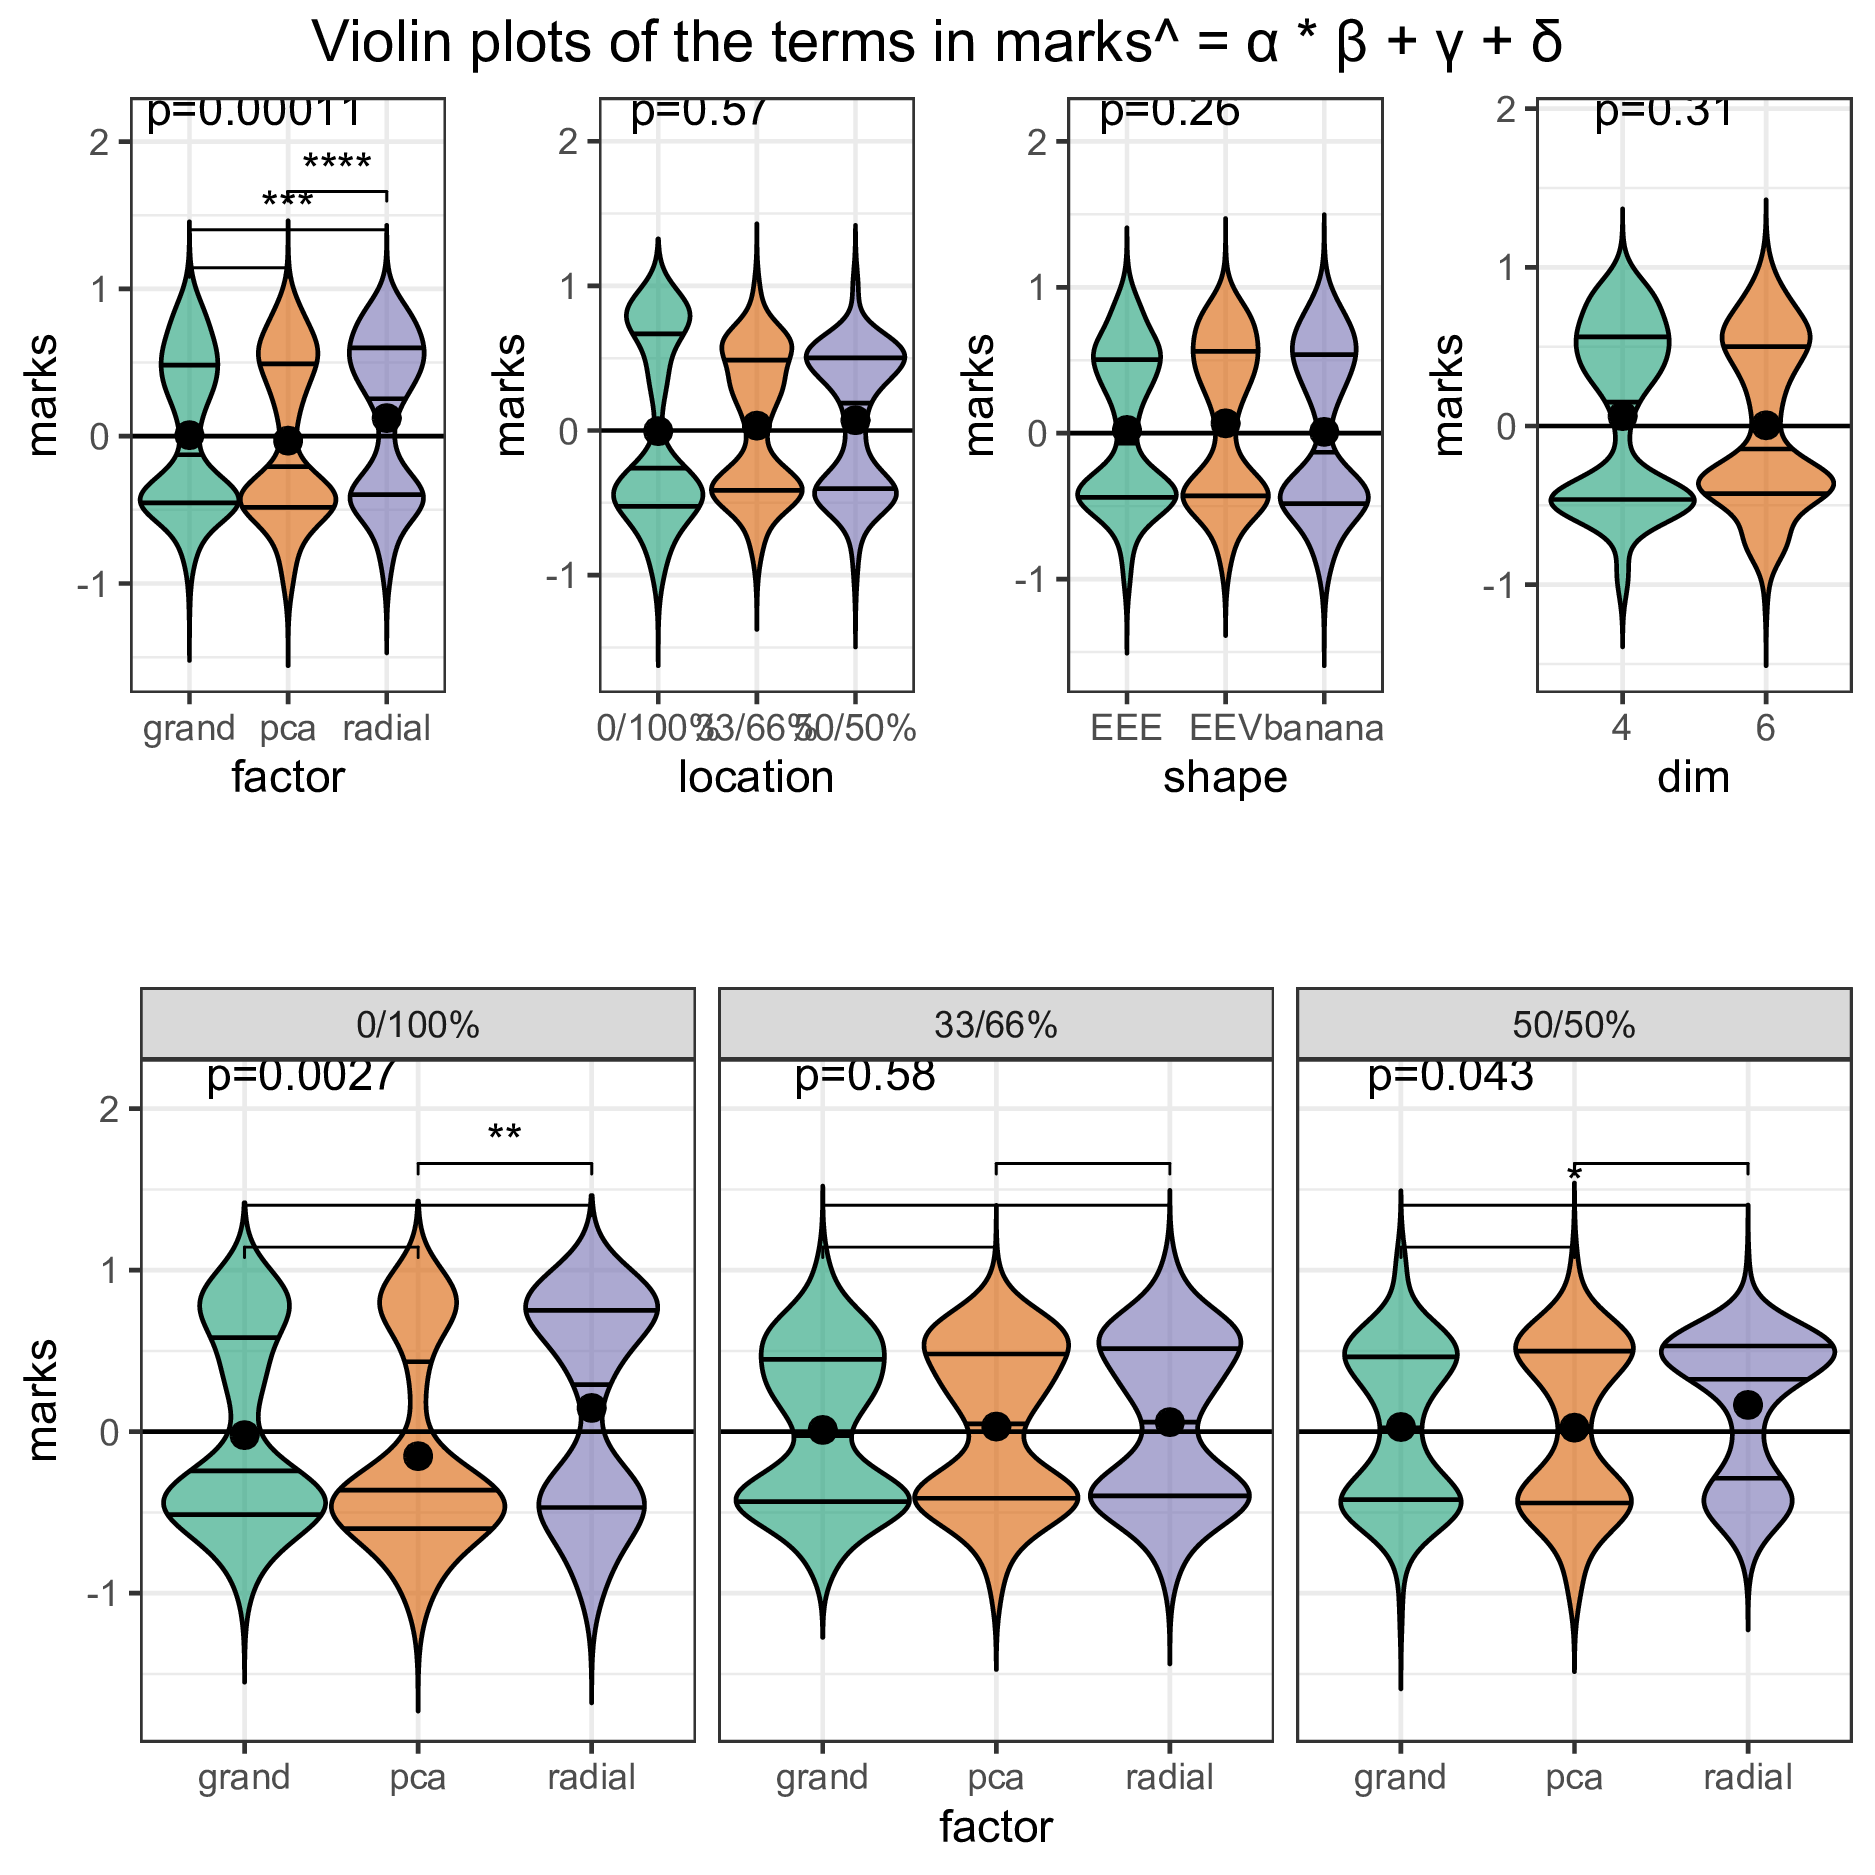
\includegraphics[width=1\linewidth,]{./figures_from_script/ch4_fig5_ABcd_violins} 

}

\caption{Violin plots of terms of the model $\widehat{Y_1} = \alpha * \beta + \gamma + \delta$. Overlaid with global significance from the Kruskal-Wallis test, and pairwise significance from the Wilcoxon test, both are non-parametric, ranked sum tests suitable for handling discrete data. Participants are more confident and find the radial easier to use relative to the grand tour. Participants claim low familiarity as we expect from crowdsourced participants. Radial is more preferred compared with either alternative for this task.}\label{fig:ch4fig5}
\end{figure}

\hypertarget{subjective-measures}{%
\subsection{Subjective measures}\label{subjective-measures}}

The 84 evaluations of the post-study survey also collect 4 subjective measures for each factor. Figure \ref{fig:ch4fig6} shows the Likert plots, or stacked percentage bar plots, alongside violin plots with the same non-parametric, ranked sum tests previously used. Participants preferred to use radial for this task. Participants were also more confident of their answers and found radial tours easier to use compared with the grand tour. All factors have reportedly low familiarity something we expect from crowdsourced participants.

\begin{figure}

{\centering 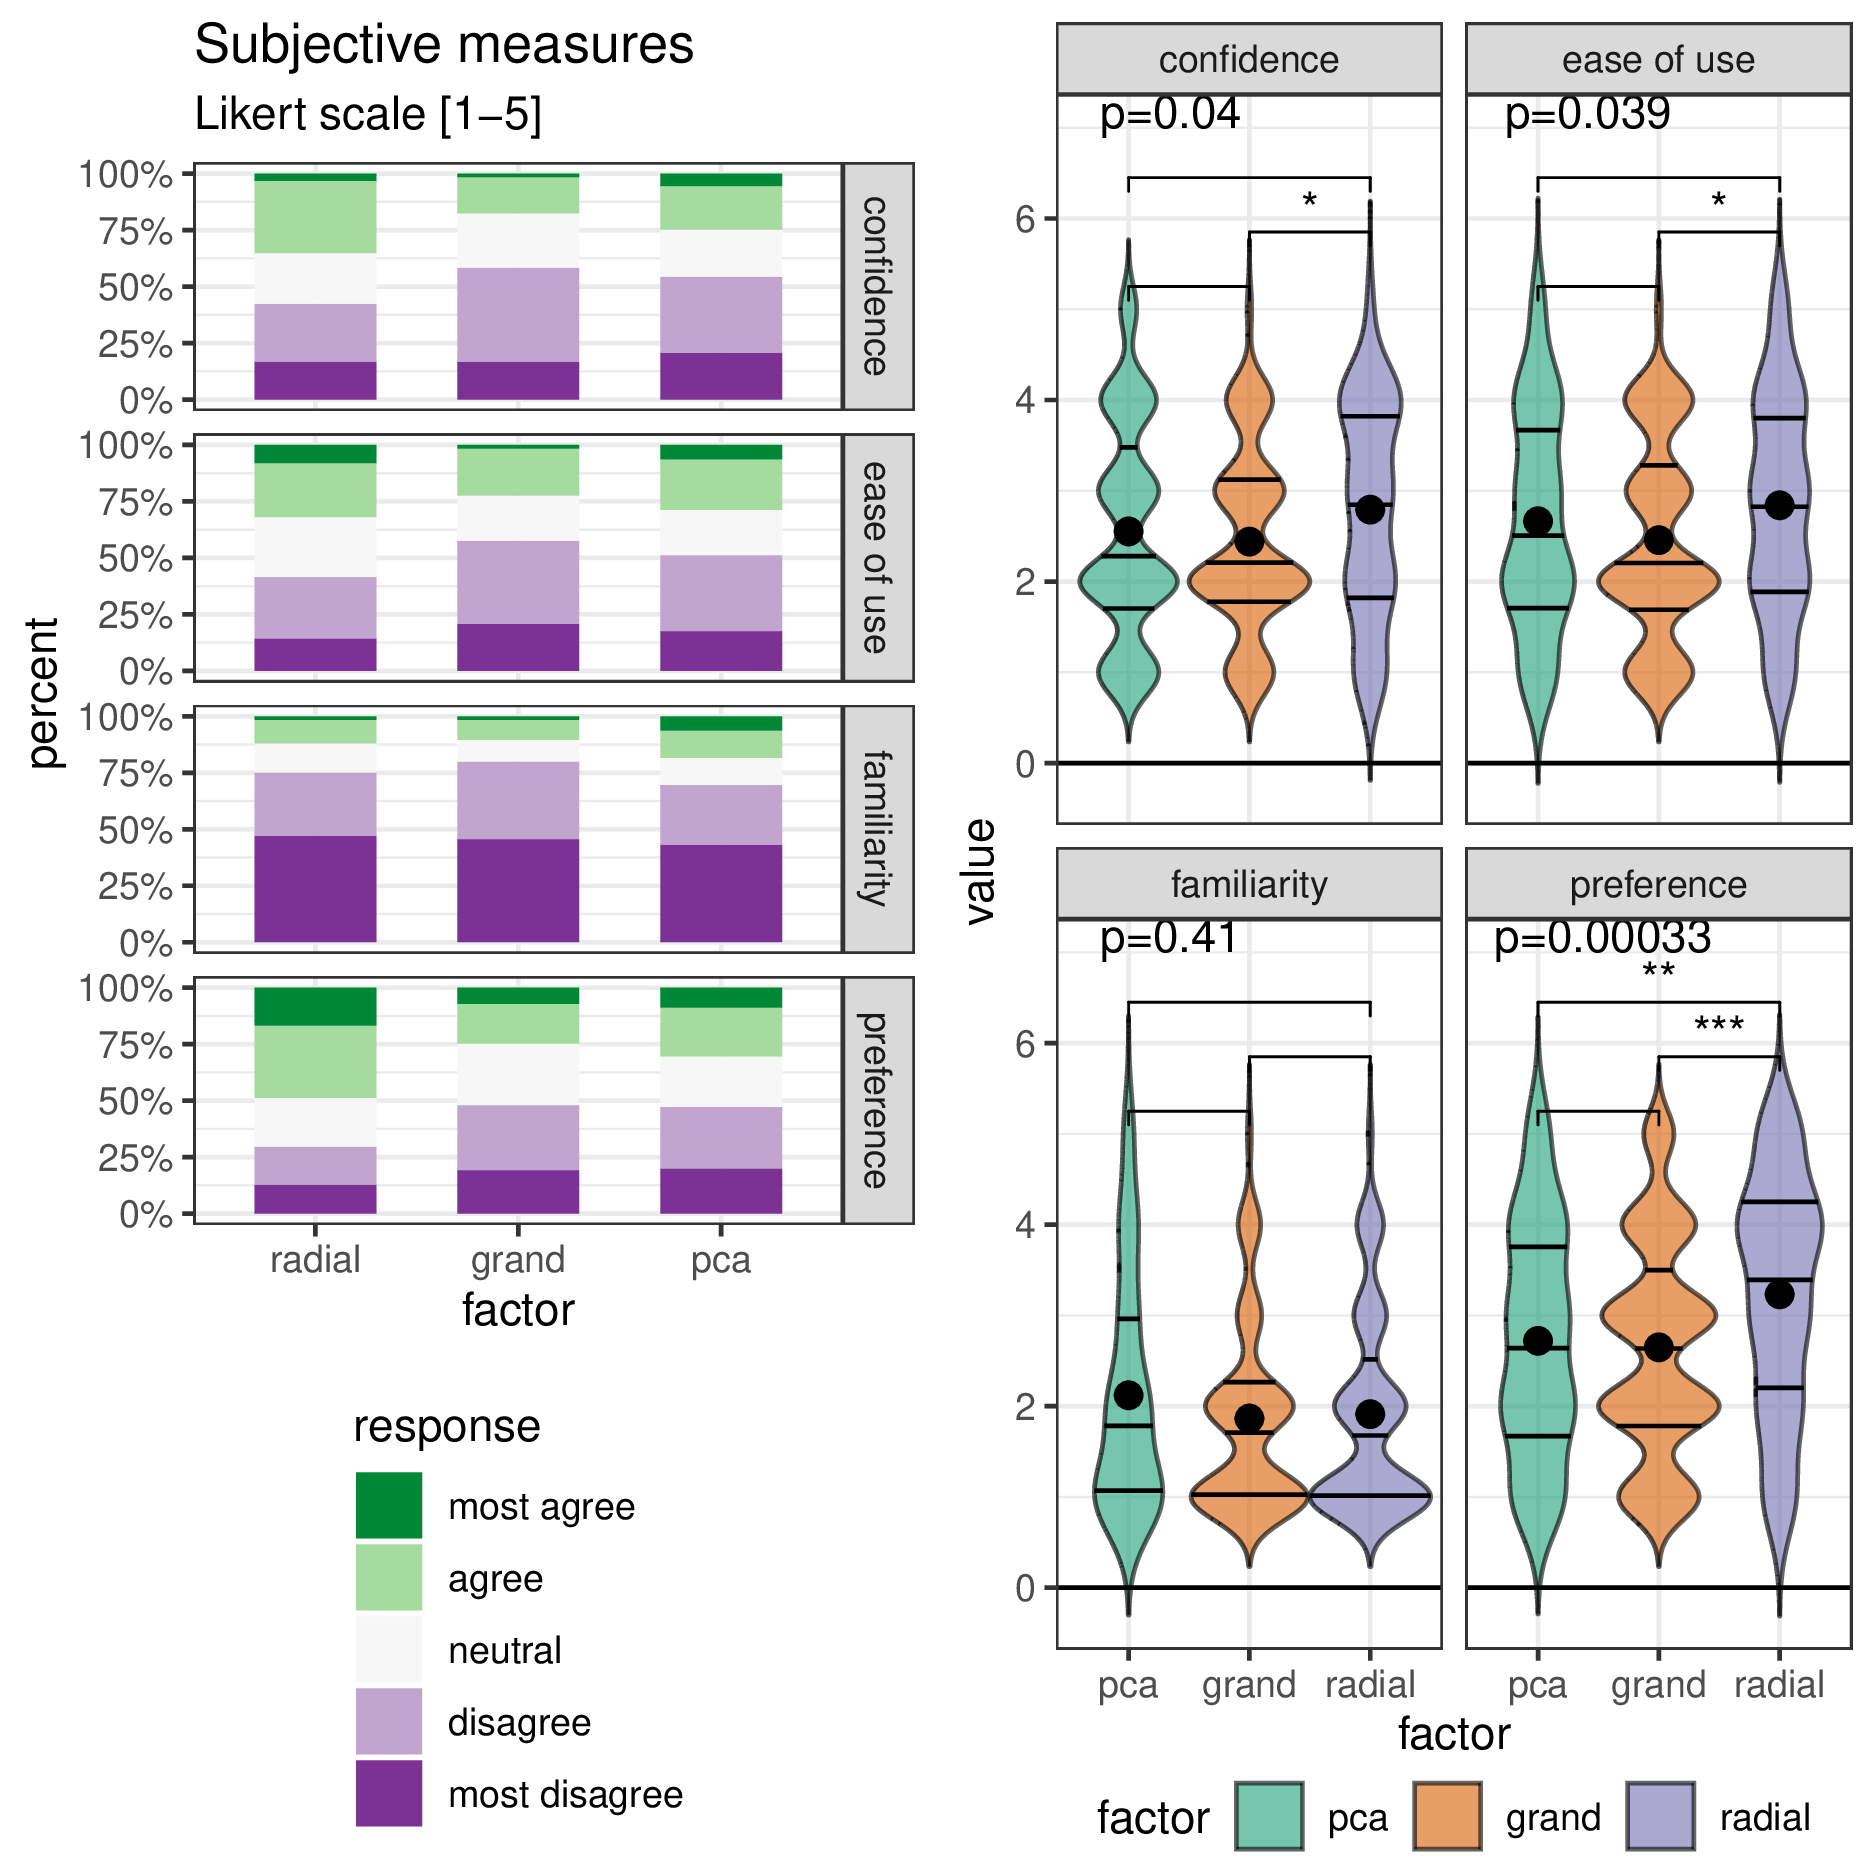
\includegraphics[width=1\linewidth,]{./figures_from_script/ch4_fig6_subjective_measures} 

}

\caption{The subjective measures of the 84 responses of the post-study survey, 5 discrete Likert scale levels of aggrement. (L) Likert plots (stacked percent bar plots) with (R) violin plots of the same measures. Violin plots are overlaid with global significance from the Kruskal-Wallis test, and pairwise significance from the Wilcoxon test, both are non-parametric, ranked sum tests.}\label{fig:ch4fig6}
\end{figure}

\hypertarget{sec:conclusion}{%
\section{Conclusion}\label{sec:conclusion}}

Above we discussed an \(n=108\), with-in participant user study comparing the efficacy of 3 linear projection techniques. The participants performed a supervised cluster task, specifically the identification of which variables contribute to the separation between 2 target clusters. This was evaluated evenly over 4 block parameterizations. In summary, we find that radial tour increases accuracy while the grand tour decreases the time it takes to perform this task. These effects are large relative to the other block parameterizations, but smaller than the random effect of the participant. Radial tour was subjectively most preferred, lead to more confidence in answers, and is easier to use than alternatives.

There are several ways that this study could be extended. In addition to expanding the support of the block parameterizations, more interesting directions include: type of the task, visualizations used, and experience level of the target population. It is difficult to achieve good coverage given the number of possible permutations. Be sure to step back and plan the target support of your block parameters. Keep in mind the volume and quality of responses from participants especially when crowdsourcing. These planning steps are useful for navigating when the complexity of the application details.

\hypertarget{sec:spinifex}{%
\section{Accompanying tool: radial tour application}\label{sec:spinifex}}

To accompany this study we have produced a more general use tool to perform such exploratory analysis of high dimensional data. The R package, \{spinifex\}, \autocite{spyrison_spinifex_2020} contains a free, open-source \{shiny\} \autocite{chang_shiny_2020} application. The application allows users to upload, perform limited preprocessing, and interactively explore their data via interactive radial tour. The .html widget produced is a more interactive variant relative to the application in the user study. Screencaptures and more details are provided in the appendix. Data can be imported from .csv, .rds, or .rda format, and projections. Run the following R code to run the application locally.

\begin{Shaded}
\begin{Highlighting}[]
\FunctionTok{install.packages}\NormalTok{(}\StringTok{"spinifex"}\NormalTok{, }\AttributeTok{dependencies =} \ConstantTok{TRUE}\NormalTok{)}
\NormalTok{spinifex}\SpecialCharTok{::}\FunctionTok{run\_app}\NormalTok{(}\StringTok{"radial\_tour"}\NormalTok{)}
\end{Highlighting}
\end{Shaded}

\hypertarget{sec:acknowledgments}{%
\section{Acknowledgments}\label{sec:acknowledgments}}

This research was supported by an Australian Government Research Training Program (RTP) Scholarship. This article was created in R \autocite{r_core_team_r:_2020} and \{rmarkdown\} \autocite{xie_r_2018}. Visuals were prepared with \{spinifex\}. All packages used are available from the Comprehensive R Archive Network (CRAN) at \url{https://CRAN.R-project.org/}. The source files for this article, application, data, and analysis can be found at \url{https://github.com/nspyrison/spinifex_study/}. The source code for the \{spinifex\} package and accompanying shiny application can be found at \url{https://github.com/nspyrison/spinifex/}.

\hypertarget{ch:cheem}{%
\chapter{Application of the radial tour to model-agnostic local explanations}\label{ch:cheem}}

THIS CHAPTER IS CURRENTLY BEING EDITED IN IT's OWN REPOSITORY, THIS VERSION IS OUT OF DATE.

TODO:XXX Segue.

\hypertarget{sec:intro}{%
\section{Introduction}\label{sec:intro}}

This work is concerned with linear projections of multivariate data. More specifically, we focus on the class of visualizations known as \emph{tours} \autocite{cook_grand_2008,lee_review_2021}. Tours are viewed near-continuously through small changes to the projection basis. There are many variants of tours. We focus on one of the variants, \emph{radial tours} \autocite{cook_manual_1997,spyrison_spinifex_2020}. Radial tours can be used to control or steer the projection basis, while other tour variants select bases randomly or optimize an objective function. Because of this unique attribute, \emph{user interaction} is another key aspect of interest in this work.

Radial tours change the basis by selecting one variable and specifying how to change its contribution to the current projection. By controlling the contribution of a single variable, a user can explore its sensitivity to the structure of the projection and identify which variables are ultimately most important to the structure in question. In the work addressing RO\#1, we improve upon the geodesic interpolator for use in the radial tour, and apply it in an open-source \texttt{R} package, \texttt{spinifex}, this package facilitates making radial tours and extends the graphics packages interoperability for itself and the tours made from the existing package \texttt{tourr}.

Next, we substantiated the efficacy of radial tours as compared with user-selected, discrete combinations of principal components \autocite{pearson_liii._1901} and continuous projections without interaction with the \emph{grand tour} \autocite{asimov_grand_1985}. We conducted an \(N=108\) within-participant user study, where all participants use each of these visual factors. This is performed over balanced trials across the other experimental factors: location, shape, and dimension of the data. This addresses the second research question.

In our latest work, we want to see if we can apply the radial tour to aid the interpretability of black-box models. Such models have a non-linear space making them hard to interpret or understand. One recent branch in explainable artificial intelligence \autocite[XAI,][\textcite{arrieta_explainable_2020}]{adadi_peeking_2018} is the use of local explanations or the attribution of the variables for one observation of a black-box model. We use such an explanation to form a 1D basis and perform radial tours to explore how the SHAP values behave differently for misclassified observations against neighboring correctly classified observations.

\hypertarget{motivation}{%
\section{Motivation}\label{motivation}}

The term exploratory data analysis (EDA) was coined by \textcite{tukey_exploratory_1977}, who leaves it as an intentionally broad term that encompasses the initial summarization and visualization of a data set before a testing hypothesis has been formulated. This is a critical first step for understanding and becoming familiar with data and validating model assumptions. It may be tempting to review a series of summary statistics to check model assumptions. However, there are known datasets where the same summary statistics miss glaringly obvious visual patterns \autocite{anscombe_graphs_1973,matejka_same_2017}. It is easy to look at the wrong, or incomplete set of statistics needed to validate assumptions. Data visualization is crucial in EDA, it \emph{forces} you to see details and peculiarities of the data which are opaque to numeric summarization, or more nefariously, obscure their true values. Data visualization does and must remain a primary component of data analysis and model validation.

studies/support --\textgreater{}
While static documents are the norm, there are sizable benefits of user interaction. Interactive data visualization shift the locus of control back to the user, inviting them to explore and interact with the data, and offers a compact way to explore a wider range of dimensions, questions as they arise, which helped to keep the curiosity and the interest of the user.

With the emerging field of XAI, the constant tension between the interpretability of a model and its predictive power is receiving more attention. Linear models are the champions of interpretability with modest accuracy while increasing complex models improve accuracy but they can scarcely be interpreted even by experienced practitioners. One way to gain insight into a model is to focus on the local vicinity of one observation, and explain the variable weighting around that location, in an agnostic non-linear model. We call this observation level variable weights a \emph{local explanation}. There are various such local explanations, many are tied to specific classes of models, while others are model-agnostic.

We know that data visualization is important in EDA and assumption validation. User interaction allows us to explore widely and quickly while allowing us to explore ideas as they arise. These 2 elements were especially important to consider from the work addressing RO\#1 as it forms a foundation to build on in further work. The efficacy of radial tours was supported by a user study in response to the second objective. In the latest work, we apply tours in tandem with local explanations to extend the interpretability of black-box models, to address RO\#3.

\hypertarget{extending-the-interpretation-of-black-box-models-with-the-use-of-interactive-continuous-linear-projections}{%
\section{Extending the interpretation of black-box models with the use of interactive continuous linear projections}\label{extending-the-interpretation-of-black-box-models-with-the-use-of-interactive-continuous-linear-projections}}

Local explanations describe the linear variable weights in the vicinity of an observation in \(p-dim\) space. Local explanations are point-measurements of the weights for each variable describing the importance to the prediction at that point. In a highly non-linear space, the importance of the variables may change rapidly with even a small change in the explanatory variables. There are several \emph{model-agnostic} local explanations such as LIME \autocite{ribeiro_why_2016}, and SHAP \autocite{lundberg_unified_2017}. In practice, this application can be used with any model and compatible local explanation. However, below we apply and discuss SHAP values extracted from a random forest model.

\hypertarget{how-a-shap-value-is-calculated}{%
\subsection{How a SHAP value is calculated}\label{how-a-shap-value-is-calculated}}

We use FIFA soccer data \autocite{leone_fifa_2020} to explain SHAP values. We use 5000 player-observations of 9 aggregate skill measures to predict that player's wages. We use SHAP to observe how the skill attribution changes for different players, which should reflect different fielding positions. Fielding position is not explicitly used in the model, but we would expect that SHAP finds a way to change the variable weights across differing skill distributions to improve the accuracy of its wage predictions.

We have trained a random forest model and wish to further explore the weightings of this non-linear model. Following the work in \autocite{biecek_dalex_2018,biecek_explanatory_2021} we can similarly extract SHAP values, highlighting that different skills are valued differently across player positions within the model. We also show ``break down'' profiles, that is additive prediction explanations, how much of each player's predicted wages is added by each of the skill evaluations. Figure \ref{fig:ch5fig1} takes a look at the SHAP and break down profiles of a star offensive and defensive player.

\begin{figure}

{\centering 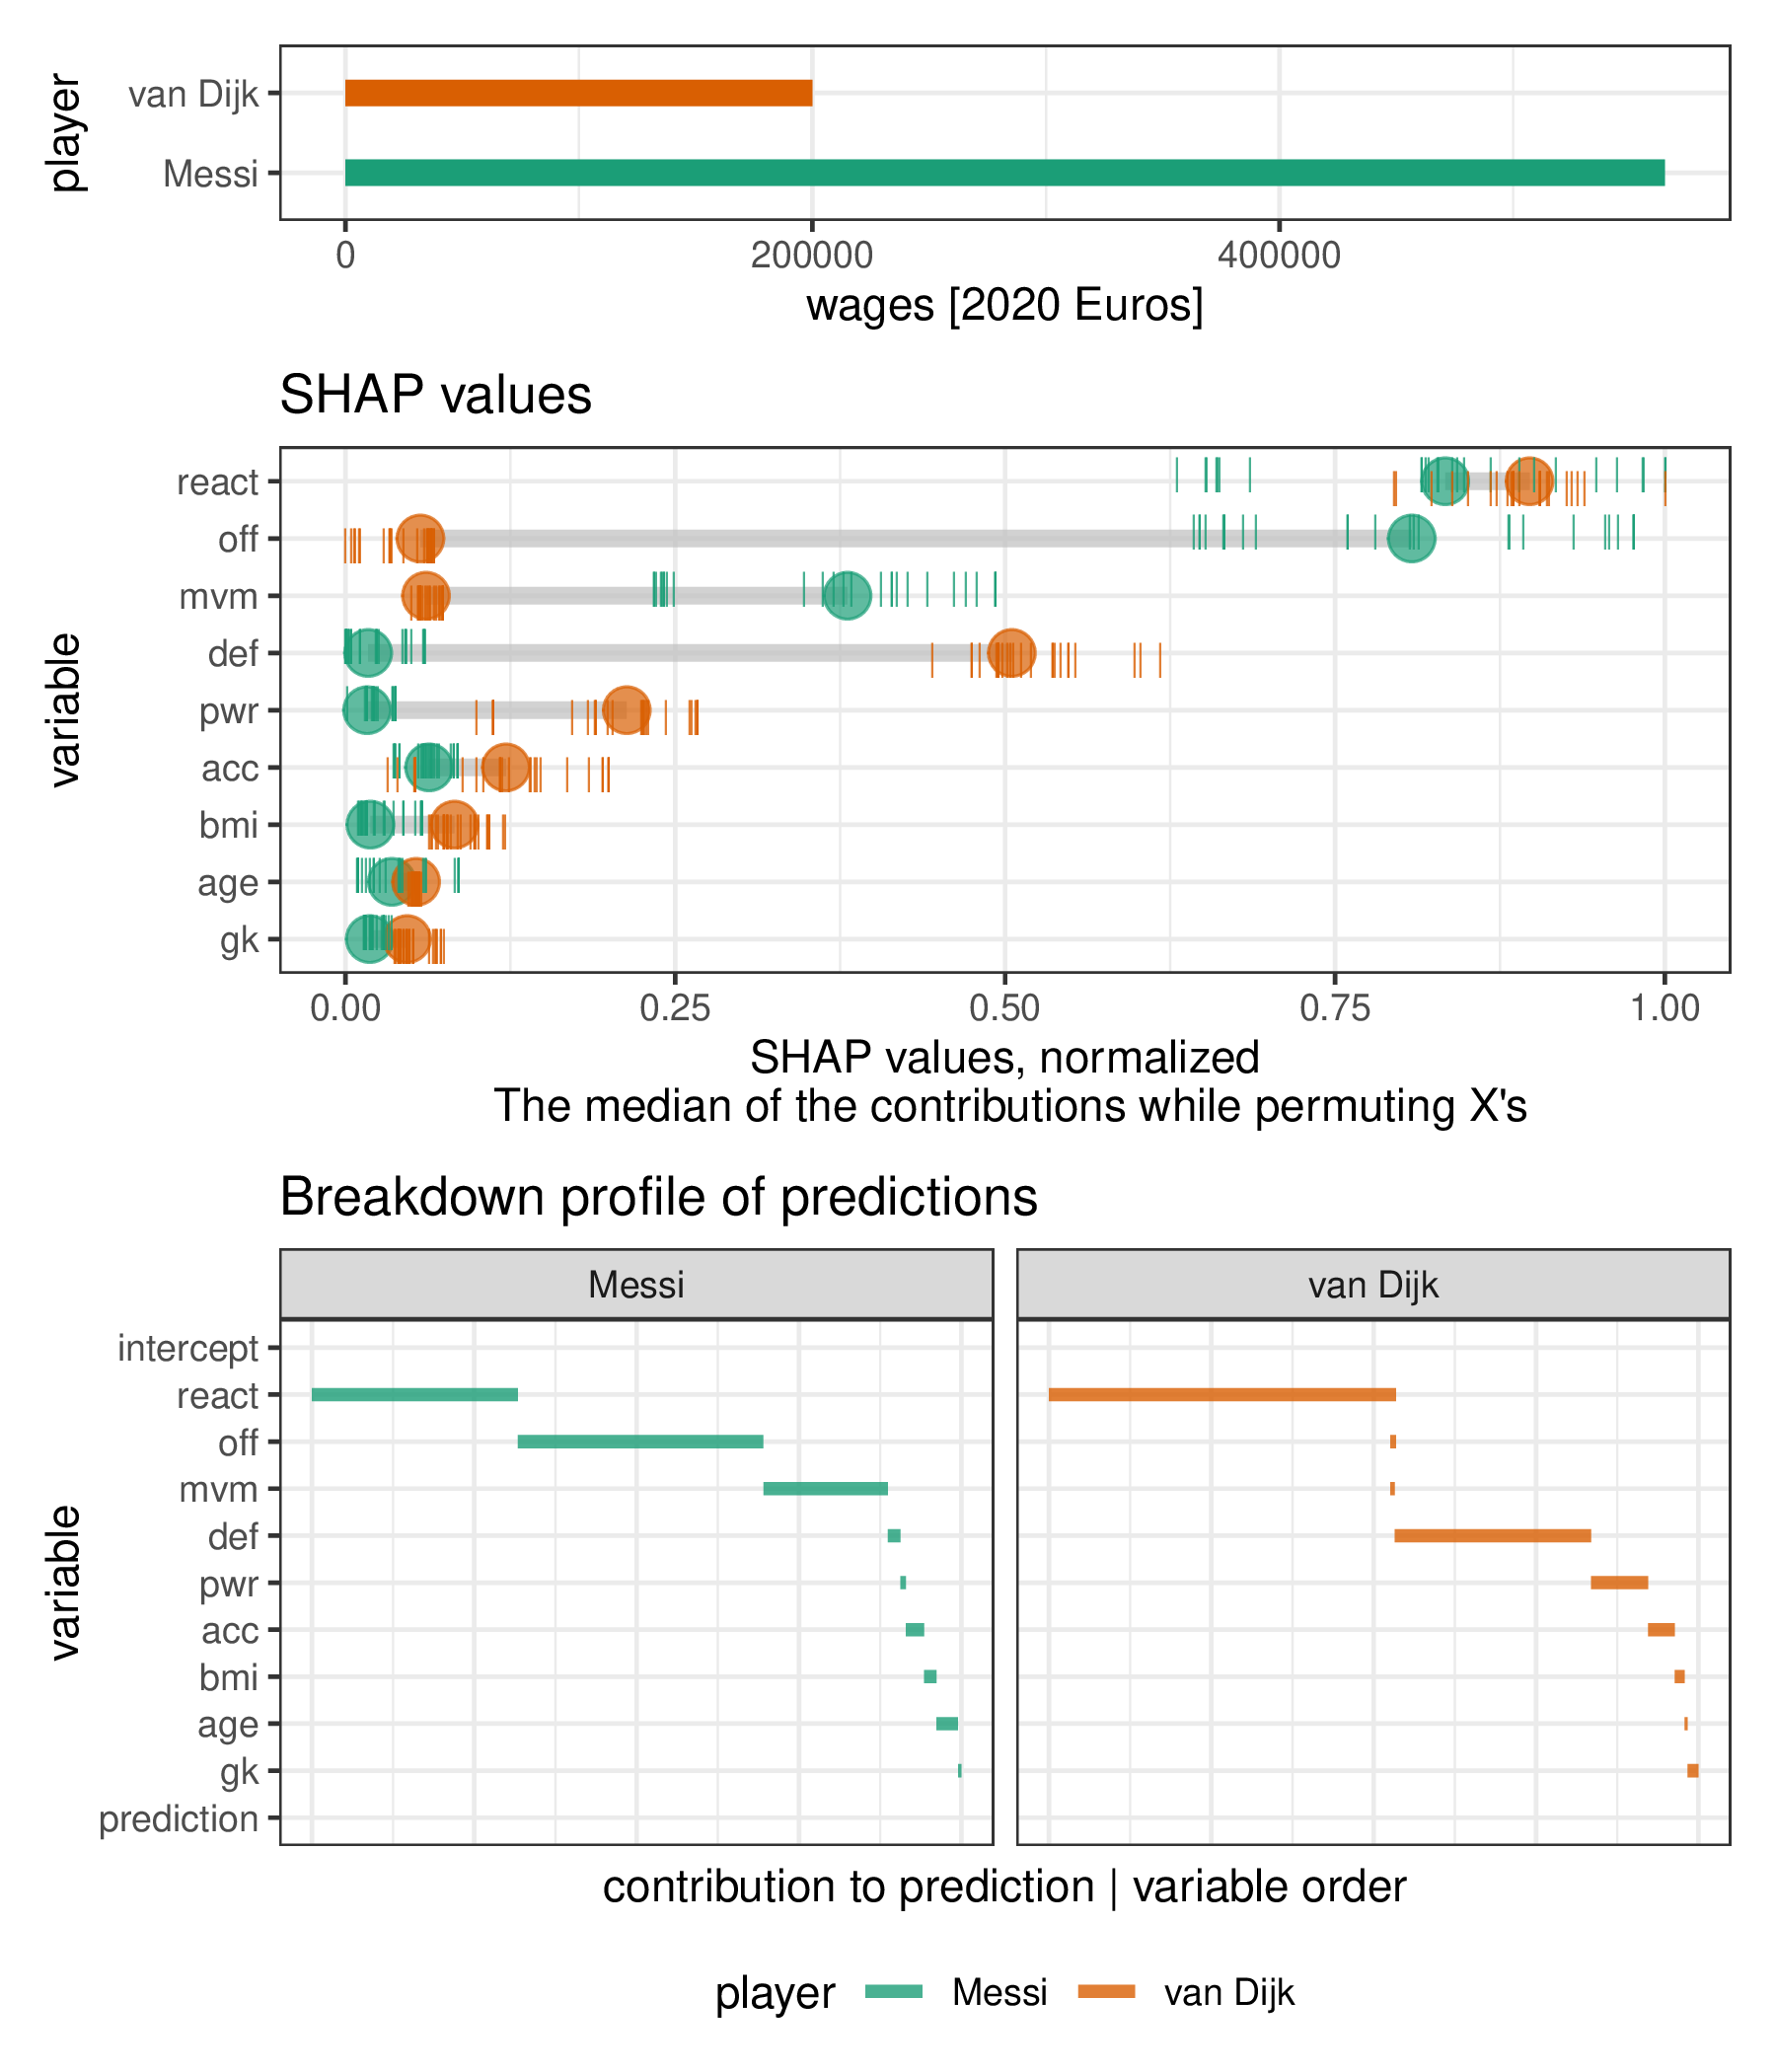
\includegraphics[width=1\linewidth,]{./figures_from_script/ch5_fig1_shap_distr_bd} 

}

\caption{SHAP values and prediction explanations of an offensive player (Messi, top) and a defensive player (van Dijk). SHAP values show a change in weights at the location of each player. Break down profiles show one order-sensitive explanation for the prediction of that observation.}\label{fig:ch5fig1}
\end{figure}

At the top of figure \ref{fig:ch5fig1} we see the relative wages of the 2 different players. SHAP uses permutations of the X variables to approximate the variable weights. In the middle, we see the distributions of the variable weightings for each player across 25 such permutations. We use the median of those distributions (large dot) as the SHAP value. We see a difference in the weights across the 2 players that makes sense considering their positions. Reaction skills are important for both players, while offensive and movement are weighted higher of the offensive player. Conversely, defensive, power, and accuracy skills are weighted higher for the defensive player. The bottom used the SHAP values to explain their relative wage predictions. We see a similar trend of the SHAP values additively explaining the difference of the global intercept to their predictions. We would expect that other offensive players have explanations closer to Messi and defensive players to lie closer to van Dijk's. The local explanations of middle fielders and goalkeepers would be expected to be different from both of these.

\hypertarget{our-application-trees-of-cheem}{%
\subsection{Our application; Trees of Cheem}\label{our-application-trees-of-cheem}}

Above, the FIFA data was used to regress continuous wages. In introducing this application, \texttt{Trees\ of\ Cheem}, we will be discussing the classification of simulated data. We simulation of 3 spherical clusters on the vertices of a triangle. The difference between the clusters is contained in the first 2 dimensions with no mean separation in another 2 noise dimensions. After extracting all observations' SHAP values, forming a SHAP \emph{matrix}, of the original dimensionality, \((n~\times~p)\).

We want to show a global view of the SHAP matrix and show how its sensitivity differs from that of the original data space. In figure \ref{fig:ch5fig2} we create an approximate of the data- and SHAP-spaces with their first 2 principal components.

This gives an orientation showing where selected observation lies. We facilitate exploration and observation identification by adding a hovering tooltip displaying row number and class (actual \& predicted) with linked brushing highlighting selected points and displaying their data tabularly below the plot.

\begin{figure}

{\centering 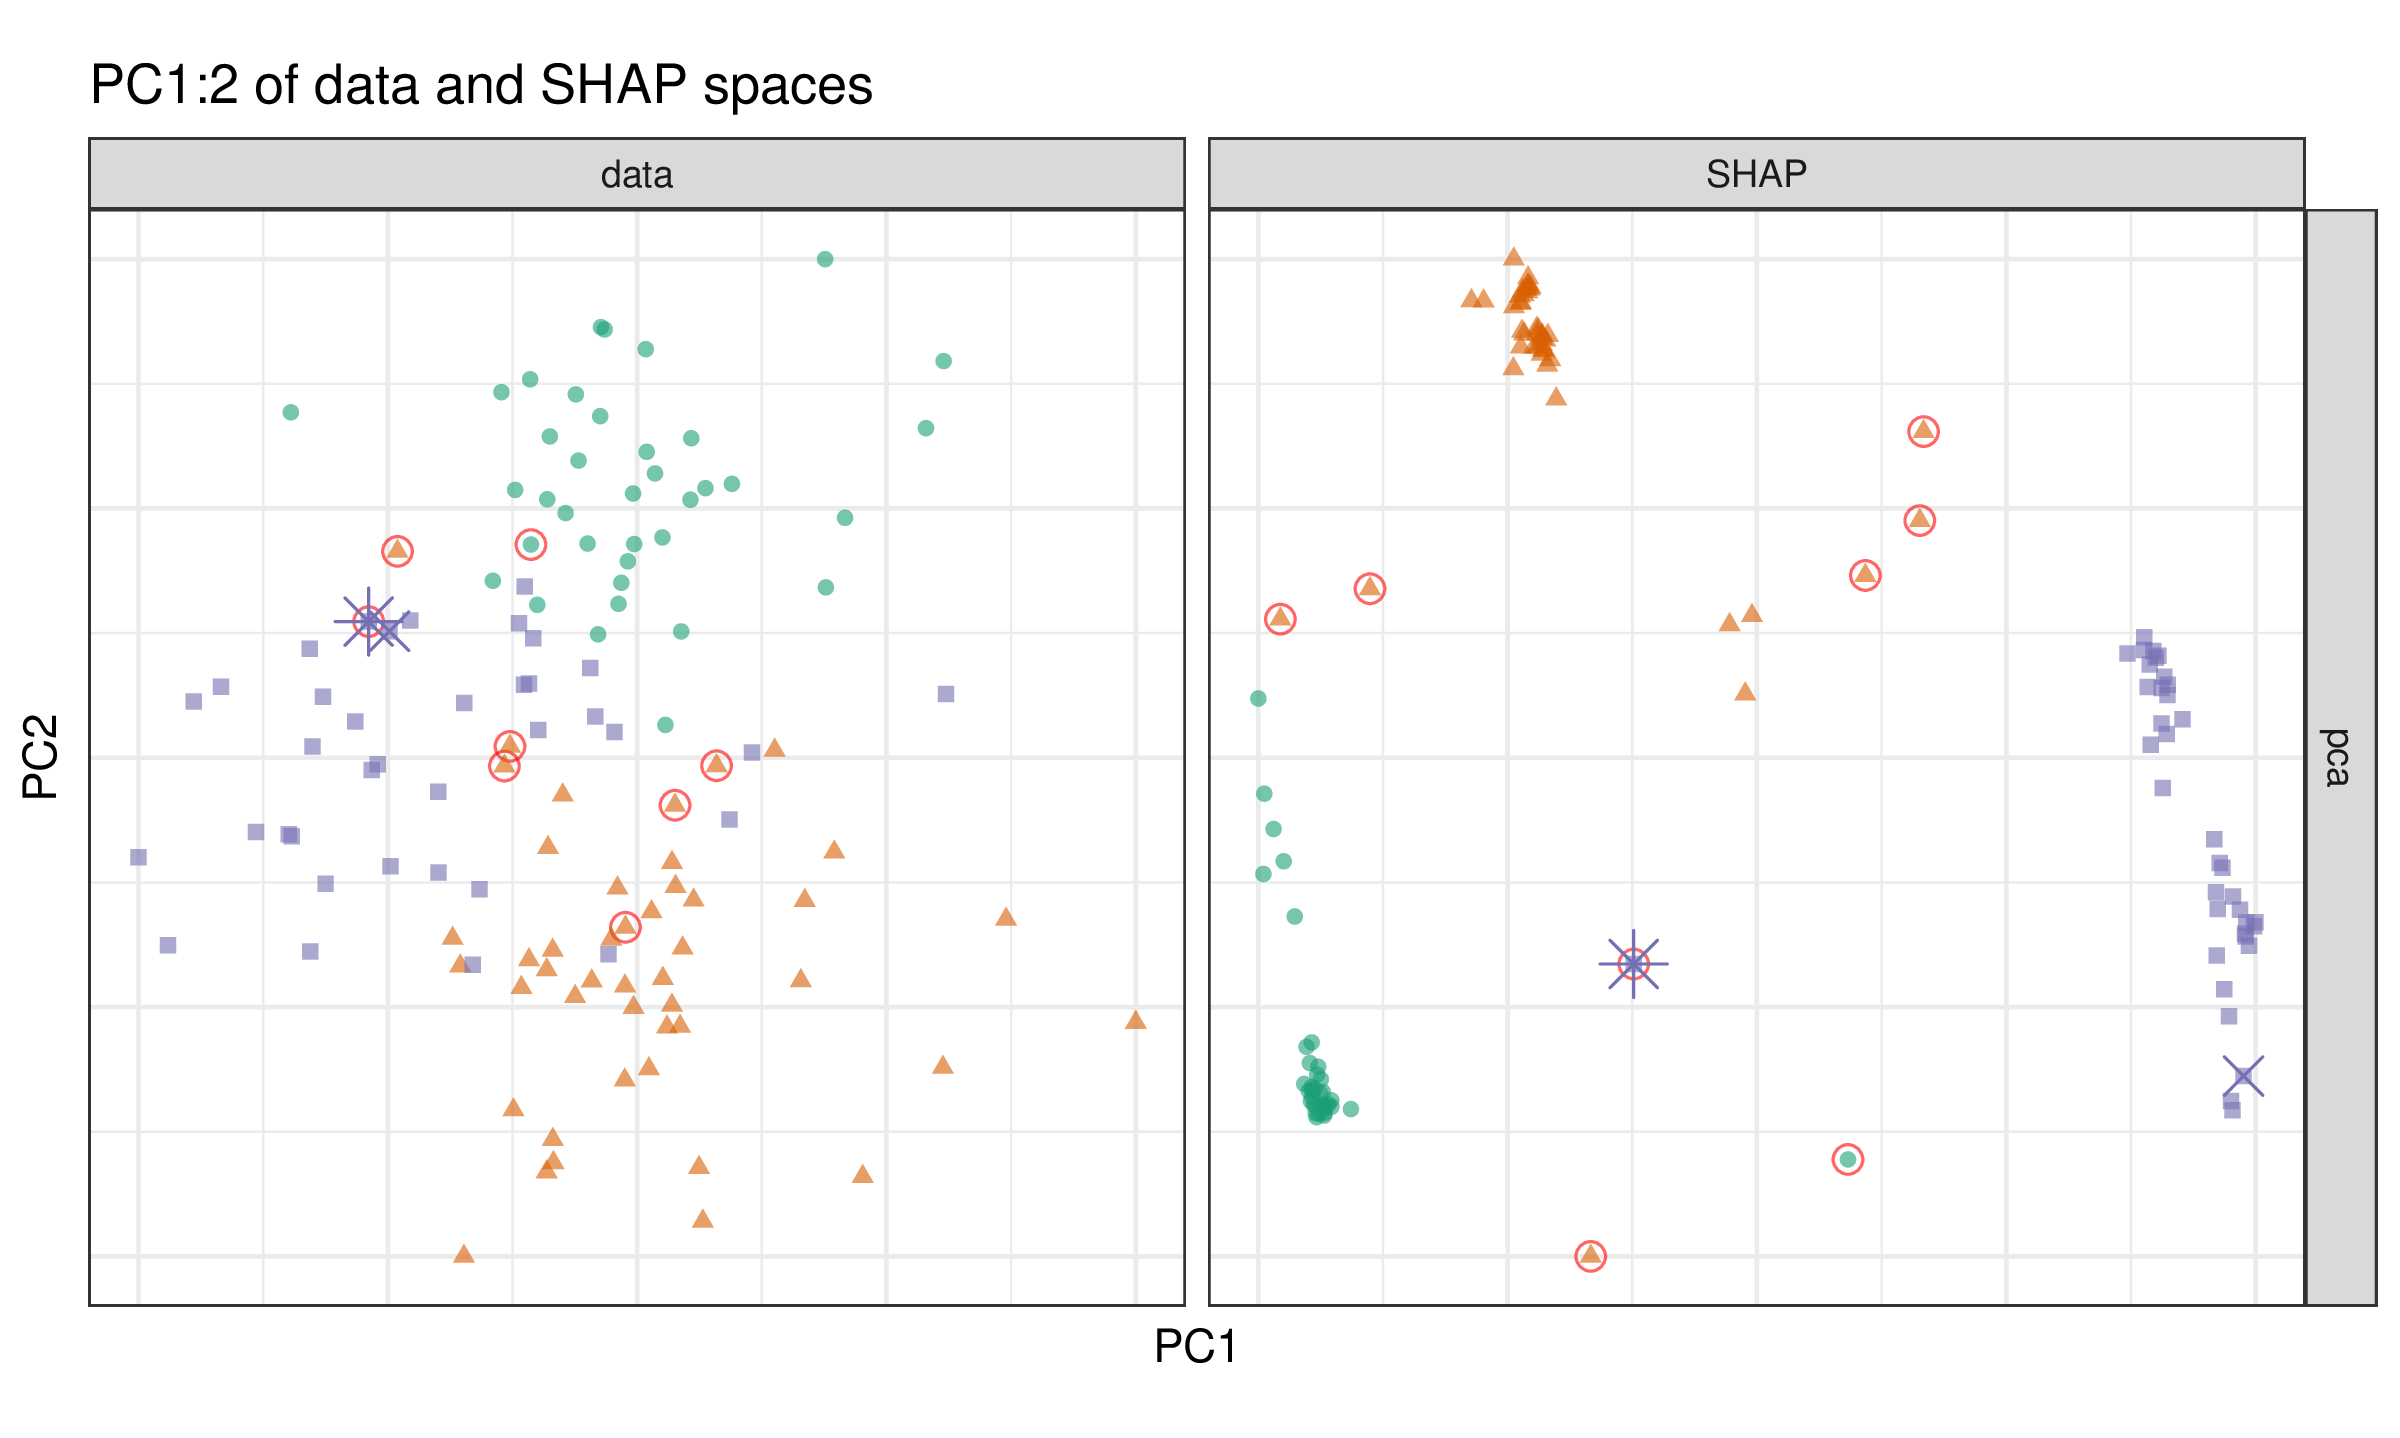
\includegraphics[width=1\linewidth,]{./figures_from_script/ch5_fig2_global_space} 

}

\caption{The first two principal conompents of the data- and SHAP-spaces (left and right respectively) of simulated data. The points are colored and shaped according to their predicted class, misclassified points are identified with a red circle. A target observation '*' is shown in contrast to a comparison point 'x', containing a nearby value in data space, but quite different SHAP space. These same 2 points are tracked in the proceeding tour.}\label{fig:ch5fig2}
\end{figure}

Looking at the SHAP space (right) the bulk of the correctly classified points are clustered in relatively small areas. This means that the distribution of their SHAP values is quite similar; the model is selecting a very tight variable contribution to explain the predicted class of each observation. Conversely, misclassified points tend to lie in between 2 clusters of correctly classified points. Using the interactive brushing and hover tooltips we confirm that these points lie between the actual and predicted classes.

Given the global view shown in figure \ref{fig:ch5fig2}, we want to look at the local explanation of primary and comparison points (highlighted as '*/x'). In this case, the primary observation is misclassified while the comparison point is a correctly classified nearby point. These 2 points that are classified differently, but otherwise have very similar values in the explanatory variables, lie quite far apart in SHAP space.

\begin{figure}

{\centering 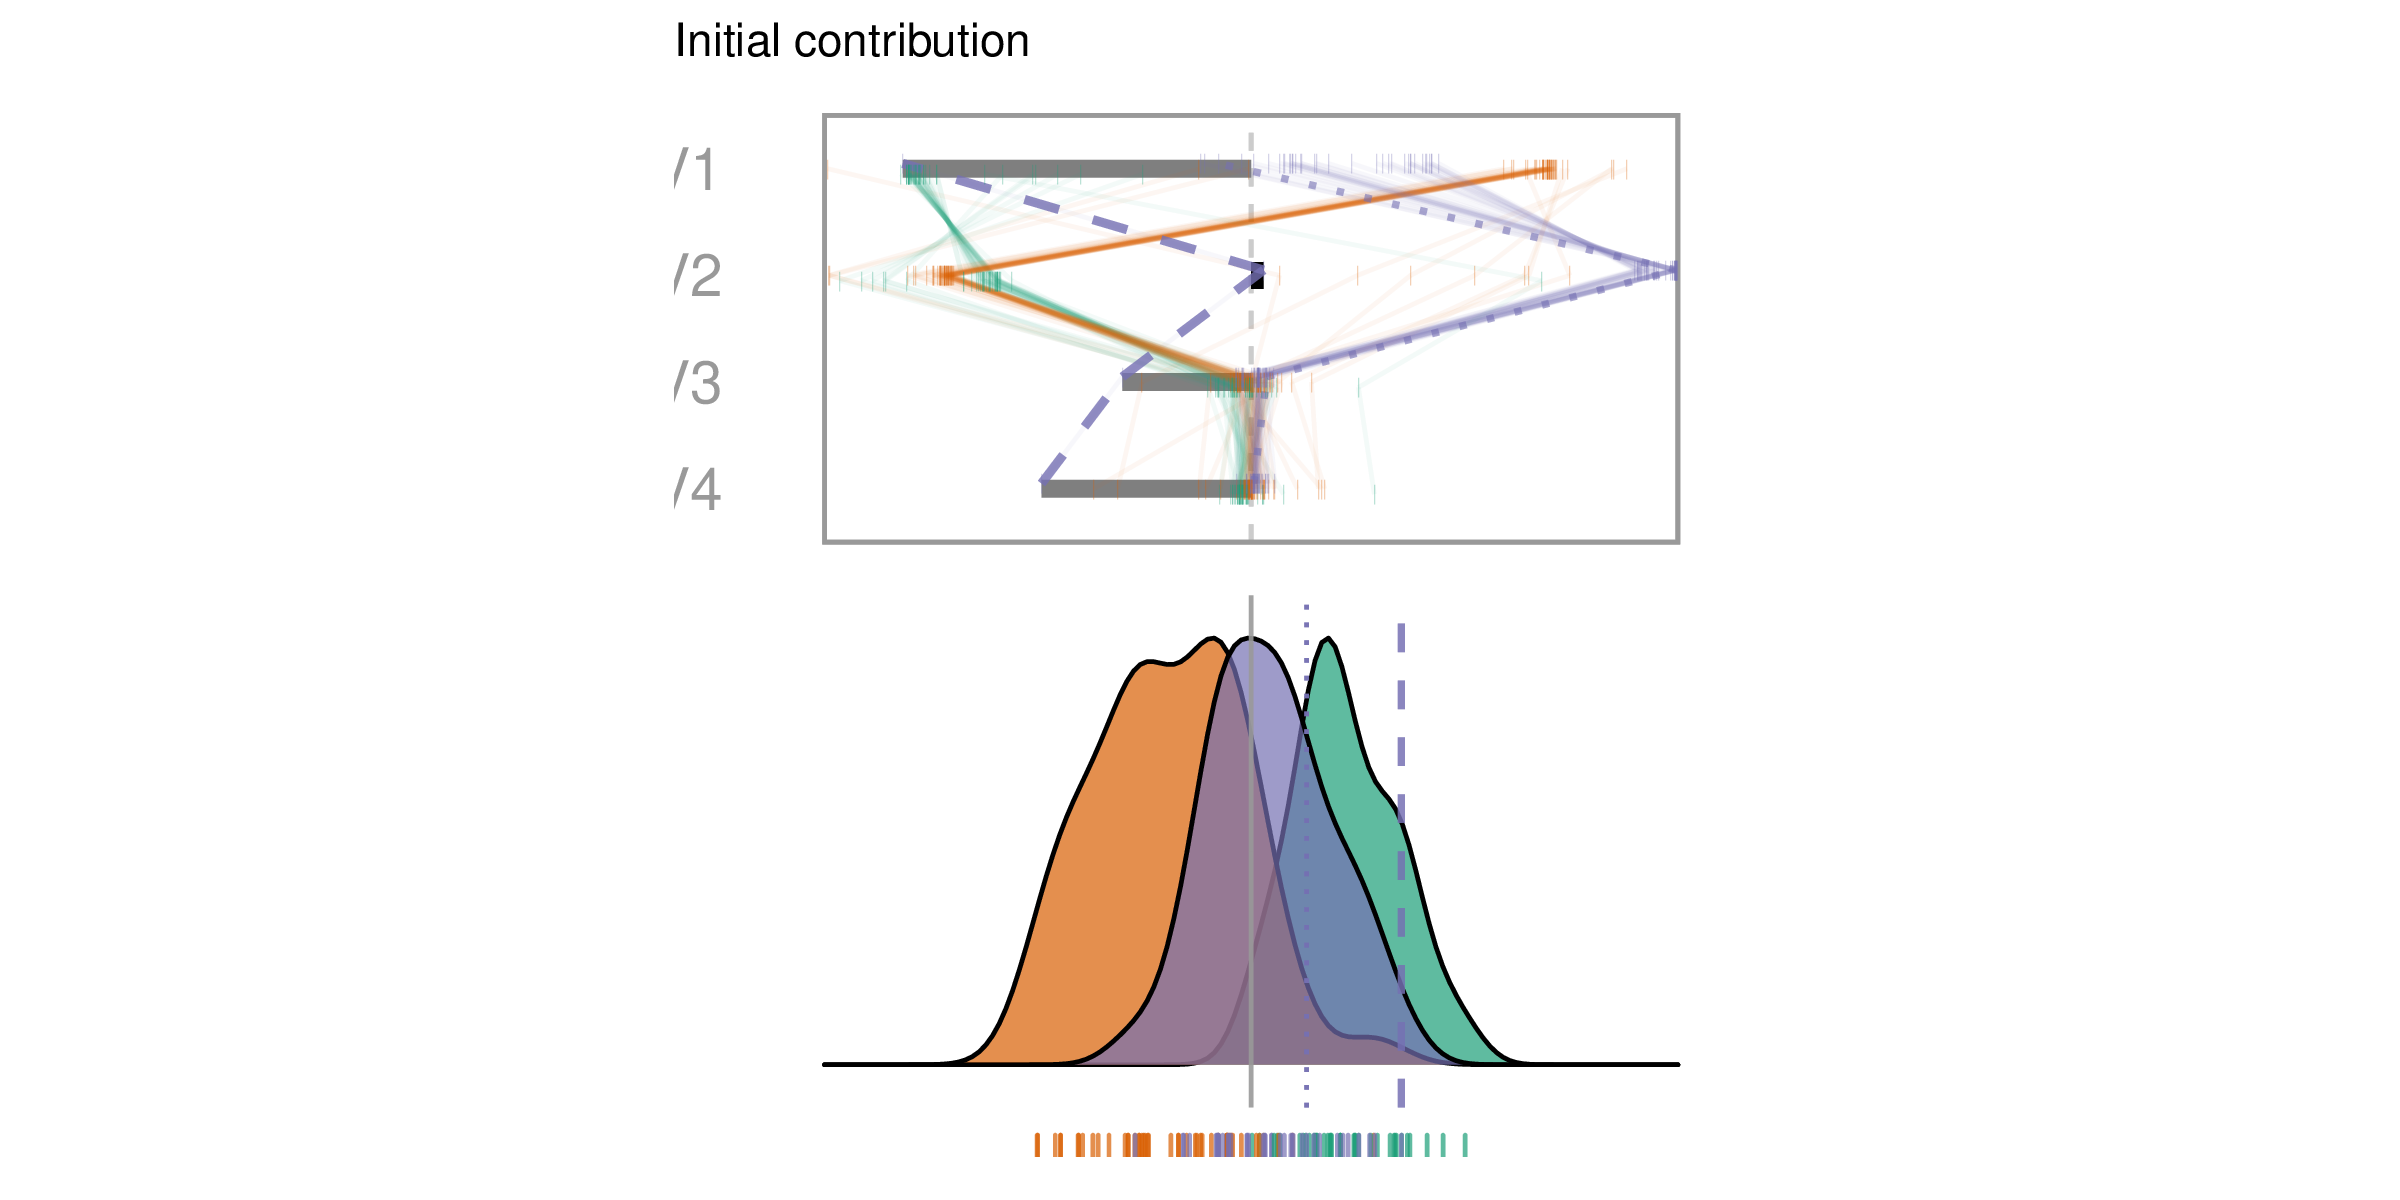
\includegraphics[width=1\linewidth,]{./figures_from_script/ch5_fig3_cheem_initial_bas} 

}

\caption{Top: 1D projection basis, the normalized SHAP values of the select observation are shown as grey/black bars. The distribution of the other observations is shown with parallel coordinate lines. The primary and comparison points ('*/x' previous) are shown as bolder dashed lines and fainter dotted lines respectively. Bottom: the 1D density and rug marks of the current projection basis.}\label{fig:ch5fig3}
\end{figure}

Now we have the global context and a comparison of the sensitivity of the SHAP spaces let's turn more toward the target observations. Figure \ref{fig:ch5fig3} highlights the same selected points, bolder dashed and fainter dotted lines (previously '*/x' points respectively). The top of the figure shows the selected observation's SHAP values as grey/black bars. The other values of the SHAP matrix are displayed as short vertical bars and joining parallel coordinate lines and are similarly colored with their predicted class. The majority of the easy-to-classify points form a relatively tight spread in the first 2 variables (signal) and more chaotic behavior in the two noise variables as we would expect. Our dotted comparison lies with the bulk of the purple class. The dashed primary point is actually a green point misclassified as a purple, its weight for V1 looks like a green point, but its V2 weight deviates and is much closer to that of a purple. V2 is the variable that is crucial to the explanation of the model for why this particular point is misclassified. In the absence of V2, our target observation is weighted much closer to the that of its true class. This is the variable we want to explore the structure of in the radial tour as indicated with the black contribution bar.

\begin{figure}

{\centering 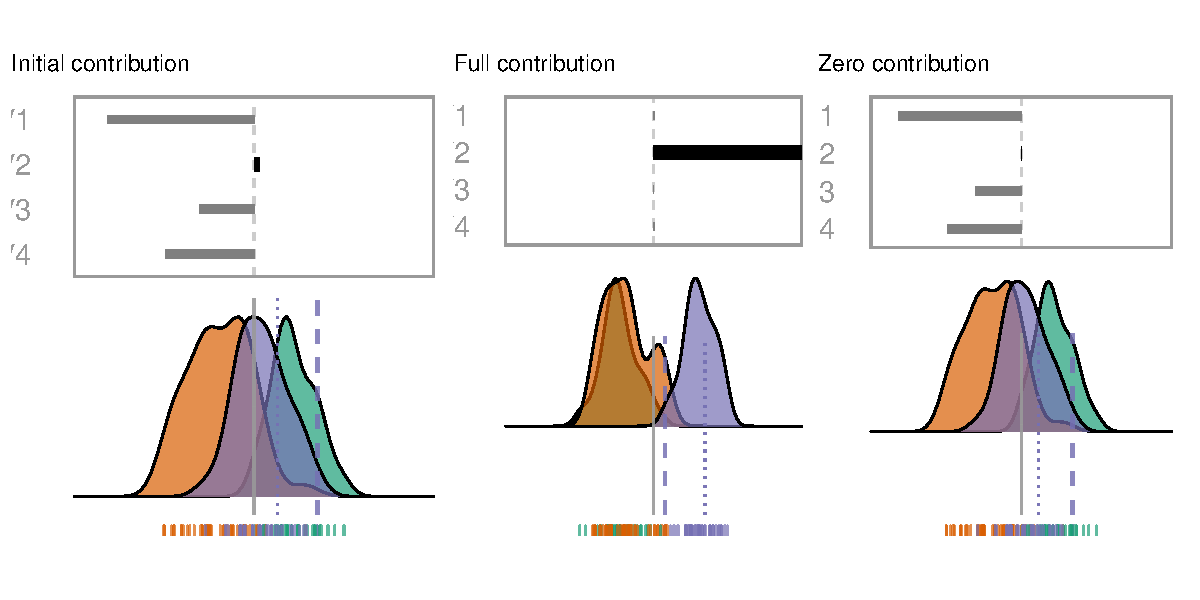
\includegraphics[width=1\linewidth,]{./figures_from_script/ch5_fig4_cheem_endpts} 

}

\caption{The first frame of the radial tour. The SHAP values of the selected observation set the initial basis, shown as the grey and black bars on top. Within class distributions of the SHAP values are shown as parallel coordinate plots next to the variable contributions. The class densities and observation positions of the 1D projection are shown on the bottom. The tour animates over small changes in the basis (top bars) as the variable with the largest contribution (weight) is rotated to have a full contribution, zero contribution, and then back to the initial contribution. Variable 2 is critical to this local explanation; In the initial contribution, both selected observations are in the middle of the purple. With a full contribution of V2 typical of most purple, our primary observation is toward the tail. When there is no contribution of variable 2, the selected observation is in the middle of the green distribution, its true class.}\label{fig:ch5fig4}
\end{figure}

Now that we have identified that V2 is the variable that deviated most from its true peer observation, we select it to rotate with the radial tour. In figure \ref{fig:cheemTour} illustrates the difference in the extremes of the contribution. The tour starts at the original contributions as described by the SHAP values (left frame). As the tour gives V2 a full contribution (middle frame) the comparison lies in the middle of the purples while the target observation is in the tails of both the purple and green (true class). In the right-most frame, the contribution from variable 2 is zero and the target variable lies in the middle of its true class. That is to say, without the contribution of variable 2 the local explanation does not seem reasonable; the selected observation looks much more like that of its true class.

This application is still maturing and has mostly focused on classification tasks. We have partial implementation of regression which will be demonstrated in the presentation, time permitting. This work is being written up to be submitted to the WHY-21 workshop, part of the NeurIPS 2021 Conference.

\hypertarget{discussion}{%
\subsection{Discussion}\label{discussion}}

We have used radial tours to improve the interpretability of black-box models. We display 2D approximations of the data to keep the global context in mind and facilitate the selection of points to focus on. After a target point have been identified, its SHAP values are used as the initial projection basis. Where the within-class distributions of the value values are displayed. The default variable selected contains the largest difference from the median of SHAP values within that point's actual classification. That is that variable that deviates the most from what would be expected from a typical correctly classified observation.

Taking a step back, it is important to remember that this visualization and analysis is sensitive to the model and local explanation; it describes them as they are, independent of their validity and quality. The insight gleaned by this is predicated on meaningful selection of model and explanation.

Turning for a minute to real-world application, developing methods to better interpret black-box models is an important and impactful challenge. Private corporations and nation-states increasingly using complex models to classify and predict their customers and citizens from loans and insurance claims to employment and credit scores, the real-world impact of highly non-linear is here to stay. Being able to see the specifics of one observation may seem small in the context of a model, but it is crucial to that instance; if misclassificated, that observation may receive an outcome a world apart from its actual peers.

\hypertarget{sec:acknowledgments}{%
\section{Acknowledgments}\label{sec:acknowledgments}}

I would like to thank Professor Przemyslaw Biecek (Warsaw University of Technology) for his time and input in suggesting to look at SHAP local explanations and try applying to the FIFA dataset.

This research was supported by an Australian government Research Training Program (RTP) scholarship. This article was created in \texttt{R} \autocite{r_core_team_r:_2020} and \texttt{rmarkdown} \autocite{xie_r_2018}.

For transparency and reproducibility, the source files are made available at \href{https://github.com/nspyrison/phd_milestones}{github.com/nspyrison/phd\_milestones}.

\hypertarget{ch:conclusion}{%
\chapter{Conclusion}\label{ch:conclusion}}

In Chapter \ref{ch:spinifex} we discussed \textbf{spinifex}. How it facilitates the preprocess transformations with \texttt{scale\_*} functions, identifies features with \texttt{basis\_*} functions, and creates manual tours. It creates a framework for layered creation of tour visuals with \texttt{proto\_*} functions that will feel at home to \textbf{ggplot2} users. Manual tours and those created from \textbf{tourr} can be rendered and exported as interactive HTML widgets, .gif, or .mp4 files. It has been downloaded over 14400 times from CRAN between 09 April 2019 and 28 November 2021. my contributions \textbf{spinifex} and \textbf{tourr} won the ACEMS Impact and Engagement Award, 2018.

Chapter \ref{ch:efficacy_radial_tour} discussed a user study comparing the radial tour against PCA and the grand tour. Participants performed a variable attribution task of the supervised cluster separation. We define an accuracy measure for this task and aditional experemental factors of location, shape, and dimensionality. I find strong evidence that use of the radial tour leads to high accurcay for this task. Using mixed model regression, I partition the error term of the model into the variation from participant's skill, and variation in difficult of the simulations due to random draws.

Now that we have evidence to support the radial tours use for variable attribution we extend their use to the further explore the local explanation of black-box models. Chapter \ref{ch:cheem} introduces an interactive global view that compares approximations of data- and attribution- spaces next to model performance. The explanations of selected observation from this global view are used as the initial basis for a radial tour to explore what support of variable contributions aggree with the explanation view. Preprocessing functions as well as interactive application are provided in a free, open-source package \textbf{cheem}.

\hypertarget{futher-extensions}{%
\section{Futher extensions}\label{futher-extensions}}

There are direct natural extension to \textbf{spinifex} such as adding adding protos, such as adding a text table of the basis, 2D density contours, convex hulls, alpha hulls, and an `high density region' display where the bulk of the data is shown as density contour, while the outer most observations are displayed as points \autocite{hyndman_computing_1996}.

Similarly, \textbf{cheem} could be generalized to a broader range models and local explanations. The models and local explanations facilitated by \texttt{DALEX::explain()} seems to be a good starting point {[}\textcite{biecek_dalex_2018}; biecek\_explanatory\_2021{]}. Alternatively there may be other statistics that better show the structure identified by explanations that could be added.

Experiencing tours as 3D scatterplots on 2D display, or in extended reality with steroscopically true head tracking may be fruitful. This has been partial explored {[}\textcite{nelson_xgobi_1998}; yang\_3d\_1999; yang\_interactive\_2000{]}, though it would be interesting see an modern implementations using WebGL, Mozilla Aframe, or Unity. One concern would be trying to keep hardware and software as generalized as possible.

In addition to application that involve one tour variant such as the applications we have discussed or \textbf{liminal} \autocite{lee_casting_2020}, a general more consolidated application with multiple linked brushing would be nice to have. Amiddedly there have been many takes on applications to facilitate the exploration of multivariate data and the audience that know and use tours remains small {[}\textcite{fisherkeller_prim-9:_1974}; \textcite{carr_explor4:_1988}; \textcite{tierney_lisp-stat:_1990}; \textcite{swayne_xgobi:_1991}; \textcite{hardle_xplore:_1995}; \textcite{carr_explorn:_1996}; \textcite{nelson_xgobi_1998}; \textcite{sutherland_orca:_2000}; \textcite{huh_davis:_2002}; \textcite{swayne_ggobi:_2003}; \textcite{wegman_visual_2003}; \textcite{jeong_ipca:_2009}, hadjar\_webvr\_2018; cordeil\_iatk\_2019{]}.

\hypertarget{other-contributions}{%
\section{Other contributions:}\label{other-contributions}}

In addition to the research discussed around the central theme of the radial tour there are other notable contributions I would mention:

\begin{itemize}
\tightlist
\item
  \emph{``Is IEEE VIS that good?'' On key factors in the initial assessment of manuscript and venue quality} \autocite{spyrison_is_2021}, A survey IEEE VIS authors, how they source articles, decide which to read, and evaluate venue quality. We find low evidence that sentiment changes across academic positions for these topics and provide commentary and discussion on the effects of ``publish or perish'' environment, standard author and journal metrics, and the need to publish ``null finding'' and replication studies.
\item
  \emph{Intraday effect of COVID-19 restrictions on Melbourne electricity consumption} \autocite{barrow_changes_2020}, We corroborate that the Victorian interday effect on energy consumption did not change, and novelly find that the intraday distribution of energy consumption does change. Namely we find a statistically significant change in the height of the morning and evening peak energy consumption that we posit is due to less strict schedules accociated with working from home, abence of commute time, or other employment changes. We were awarded 1st place of hundreds of entries in the insights category of the Melbourne 2020 Datathon.
\item
  Student volunteering at conferences: UseR!2021 - Online, CHI Down Under 2020 - Online, and UseR!2018 - Brisbane, Australia.
\end{itemize}

\printbibliography[heading=bibintoc]

\end{document}
